\chapter{Popis veličin v prostoru}

\section{Pseudometrický prostor, metrický prostor}

Mějme množinu prvků \(M\) a funkci \(d: M \times M \rightarrow \mathbb{R}\), která určuje vzdálenost dvou prvků z \(M\).

\begin{equation}
\label{eq:pseudometricky_prostor_definice_1}
\forall u \in M : d(u, u) = 0
\end{equation}

\begin{equation}
\label{eq:pseudometricky_prostor_definice_2}
\forall u, v \in M : d(u, v) = d(v, u)
\end{equation}

\begin{equation}
\label{eq:pseudometricky_prostor_definice_3}
\forall u, v, w \in M : d(u, v) \leq d(u, w) + d(w, v)
\end{equation}

Pokud funkce \(d\) splňuje podmínky \eqref{eq:pseudometricky_prostor_definice_1} - \eqref{eq:pseudometricky_prostor_definice_3}, pak se nazývá pseudometrika a dvojice \((M, d)\) pseudometrický prostor.

Podmínka \eqref{eq:pseudometricky_prostor_definice_1} říká, že vzdálenost totožných prvků je nulová. Podmínka \eqref{eq:pseudometricky_prostor_definice_2} znamená symetrii vzdálenosti a \eqref{eq:pseudometricky_prostor_definice_3} je trojúhelníková nerovnost.

Provedeme-li v rovnici \eqref{eq:pseudometricky_prostor_definice_3} subsstituci \(u = v = x, w = y\), a využijeme podmínky \eqref{eq:pseudometricky_prostor_definice_1} a \eqref{eq:pseudometricky_prostor_definice_2},
tak odvodíme nezápornost vzdálenosti.

\begin{equation}
\begin{split}
\forall x, y \in M : d(x, x) \leq d(x, y) + d(y, x) \\
\forall x, y \in M : 0 \leq 2 \cdot d(x, y) \\
\forall x, y \in M : d(x, y) \geq 0
\end{split}
\end{equation}

Pokud pseudometrický prostor splňuje navíc podmínku \eqref{eq:metricky_prostor_definice_1}, pak jej nazýváme metrickým prostorem.

\begin{equation}
\label{eq:metricky_prostor_definice_1}
\forall u, v \in M : d(u, v) = 0 \rightarrow u = v
\end{equation}

V~pseudometrickém prostoru tedy mohou existovat různé prvky s~nulovovou vzdáleností, v~metrickém prostoru je to vyloučeno.

\section{Euklidovský prostor, kartézský systém souřadnic}

Začněme definicí Euklidovského prostoru.

\begin{fact}
Definice: Euklidovský prostor \(E_n\) je metrický prostor, jehož prvky jsou body, v~němž můžeme zavést kartézský systém souřadnic a~v~němž platí metrika daná vztahem \eqref{eq:euklidovsky_prostor_metrika}.

\begin{equation}
\label{eq:euklidovsky_prostor_metrika}
d(A, B) = \sqrt{\sum_{i=1}^{n} (B_i - A_i)^2}
\end{equation}
\end{fact}

Euklidovský prostor je tedy prostor tvořený body. Můžeme zde zavést kartézský systém souřadnic, který každému bodu \(X\) přiřazuje \(n\)-tici reálných čísel \(X_i\). Říkáme, že se jedná o~\(n\)-rozměrný prostor.
Kartézský systém souřadnic není jediný možný, později si ukážeme, jak zavést jiné systémy souřadnic. Je pravděpodobné, že čtenář je s~kartézskou soustavou souřadnic podrobně seznámen. Předpokládejme ale nyní,
že o~ní nic nevíme a~ukážeme si, co vše lze z~rovnice \eqref{eq:euklidovsky_prostor_metrika} odvodit.

Především si všimněme, že ve vztahu \eqref{eq:euklidovsky_prostor_metrika} vystupují pouze rozdíly souřadnic. To znamená, že máme-li soustavu bodů,
pak přičtením konstantní \(n\)-tice ke všem jejich souřadnicím se vzájemné vzdálenosti bodů nezmění. Můžeme tedy soustavu bodů libovolně posunout a~jejich vzájemná poloha zůstane nezměněna. Toto je vlastnost Euklidovského
prostoru jako takového, ne jen soustavy souřadnic. To se může zdát samozřejmé, ale například teorie relativity předpokládá, že prostor může být deformovaný a~tuto vlastnost nemá. Tím jsme odvodili první fakt:

\begin{fact}
Euklidovský prostor \(E_n\) je invariantní vůči posunutí.
\end{fact}

Zavedeme označení
\eqref{eq:vektor_rozdil_bodu} a~veličinu \(\vectpoints{AB}\) nazveme vektorem. Vektor se v~některé literatuře označuje tučně, v~některé šipkou nad vektorem. V~této knize budeme vektory označovat tučně s~výjimkou vektoru
utvořeného jako rozdíl dvou bodů - ten označíme šipkou nad oněmi dvěma body. Pokud je daný vektor jednotkový (jeho velikost je rovna 1), pak nad ním
nakreslíme stříšku.

Velikost vektoru definujeme pomocí vztahu \eqref{eq:vektor_velikost}. Tím se nám definice \eqref{eq:euklidovsky_prostor_metrika} zjednoduší na \eqref{eq:euklidovsky_prostor_metrika_vektor}.

\begin{equation}
\label{eq:vektor_rozdil_bodu}
\vectpoints{AB} = (B_1 - A_1, B_2 - A_2, ..., B_n - A_n)
\end{equation}

\begin{equation}
\label{eq:vektor_velikost}
|\vect{u}| = \sqrt{\sum_{i=1}^{n} u_i^2}
\end{equation}

\begin{equation}
\label{eq:euklidovsky_prostor_metrika_vektor}
d(A, B) = |\vectpoints{AB}|
\end{equation}

Graficky budeme vektor reprezentovat pomocí šipky vedoucí od počátečního ke koncovému bodu, jak je vidět na obrázku~\ref{img:vektor_graficky}.

\begin{figure}[!h]
\centering
\begin{tikzpicture}
\draw[->] (0, 0) -- (2, 2);
\draw (0, 0) node[anchor=east]{A};
\draw (2, 2) node[anchor=west]{B};
\draw (1, 1) node[anchor=south east]{\(\vectpoints{AB}\)};
\end{tikzpicture}
\caption{Vektor}
\label{img:vektor_graficky}
\end{figure}

Mějme 3 body - A, B, C. Vidíme, že \(i\)-tá souřadnice vektoru \(\vectpoints{AB}\) je \(\vectpoints{AB}_i = B_i - A_i\), \(i\)-tá souřadnice vektoru \(\vectpoints{BC}\) je \(\vectpoints{BC}_i = C_i - B_i\) a~\(i\)-tá souřadnice vektoru \(\vectpoints{AC}\) je \(\vectpoints{AC}_i = C_i - A_i = (B_i - A_i) + (C_i - B_i) = \vectpoints{AB}_i + \vectpoints{BC}_i\). Můžeme proto zavést sčítání vektorů vztahem \eqref{eq:euklidovsky_prostor_vektor_soucet}.

\begin{figure}[!h]
\centering
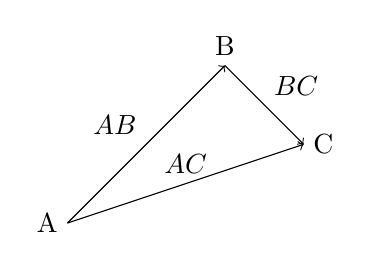
\begin{tikzpicture}
\draw[->] (0, 0) -- (2, 2);
\draw[->] (2, 2) -- (3, 1);
\draw[->] (0, 0) -- (3, 1);
\draw (0, 0) node[anchor=east]{A};
\draw (2, 2) node[anchor=south]{B};
\draw (3, 1) node[anchor=west]{C};
\draw (1, 1) node[anchor=south east]{\(\vectpoints{AB}\)};
\draw (2.5, 1.5) node[anchor=south west]{\(\vectpoints{BC}\)};
\draw (1.5, 0.5) node[anchor=south]{\(\vectpoints{AC}\)};
\end{tikzpicture}
\caption{Součet vektorů}
\label{img:soucet_vektoru}
\end{figure}

\begin{equation}
\label{eq:euklidovsky_prostor_vektor_soucet}
\vect{u} + \vect{v} = (u_1 + v_1, u_2 + v_2, ..., u_n + v_n)
\end{equation}

Dále definujme nulový vektor \(\vect{0}\) tak, že pokud jej přičteme k~libovolnému vektoru \(\vect{u}\), tak se nezmění. Tedy:

\begin{equation}
\begin{split}
\vect{u} + \vect{0} = \vect{u} \\
(u_1 + 0_1, u_2 + 0_2, ..., u_n + 0_n) = (u_1, u_2, ..., u_n ) \\
\vect{0} = (0, 0, ...)
\end{split}
\end{equation}

Vidíme, že nulový vektor má všechny složky nulové. Dosadíme-li jej do definice velikosti vektoru \eqref{eq:vektor_velikost}, tak vidíme, že \(|\vect{0}| = 0\). Navíc vidíme, že se jedná o~jediný vektor s~nulovou velikostí. Ve vztahu \eqref{eq:vektor_velikost} se totiž vyskytuje součet druhých mocnin složek vektoru. Aby tento součet mohl být nulový, tak každá složka musí být nulová. Také to tedy znamená, že nulovou metriku mohou mít jen stejné body Euklidovského prostoru. Dokázali jsme tak platnost podmínky \eqref{eq:metricky_prostor_definice_1}.

Opačný vektor \(-\vect{u}\) zavedeme jako vektor, který když přičteme k~vektoru \(\vect{u}\), tak získáme nulový vektor. Takto to bude odpovídat běžné algebře:

\begin{equation}
\begin{split}
\vect{u} + (-\vect{u}) = \vect{0} \\
(u_1 + (-\vect{u})_1, u_2 + (-\vect{u})_2, ..., u_n + (-\vect{u})_n) = (0, 0, ...) \\
-\vect{u} = (-u_1, -u_2, ..., -u_n)
\end{split}
\end{equation}

Rozdíl vektorů zavedeme jako přičtení opačného vektoru vztahem \eqref{eq:euklidovsky_prostor_vektor_rozdil}. Takto to bude odpovídat běžným pravidlům algebry.

\begin{equation}
\label{eq:euklidovsky_prostor_vektor_rozdil}
\vect{u} - \vect{v} = \vect{u} + (-\vect{v})= (u_1 - v_1, u_2 - v_2, ..., u_n - v_n)
\end{equation}

Přirozeně můžeme zavést násobení vektoru skalárem, aby odpovídalo sčítání příslušného počtu shodných vektorů. Získáme tak vztah \eqref{eq:euklidovsky_prostor_vektor_nasobeni}, který je kompatibilní se sčítáním a odečítáním vektorů:

\begin{equation}
\label{eq:euklidovsky_prostor_vektor_nasobeni}
\alpha \cdot \vect{u} = (\alpha \cdot u_1, \alpha \cdot u_2, ..., \alpha \cdot u_n)
\end{equation}


Protože jsme zavedli operace s~vektory tak, že provádíme běžné algebraické operace s~\(n\)-ticemi čísel po jednotlivých složkách, tak běžná pravidla algebry budou platit i~pro operace s~vektory. Neměla by nás proto překvapit následující pravidla. Čtenář si je může ověřit sám rozepsáním jednotlivých operací:

\begin{fact}
\begin{equation}
\label{eq:euklidovsky_prostor_definice_nuloveho_vektoru}
\vect{u} + \vect{0} = \vect{u}
\end{equation}

\begin{equation}
\label{eq:euklidovsky_prostor_definice_opacneho_vektoru}
\vect{u} + (-\vect{u}) = \vect{0}
\end{equation}

\begin{equation}
\label{eq:euklidovsky_prostor_definice_odecitani_vektoru}
\vect{u} - \vect{v} = \vect{u} + (-\vect{v})
\end{equation}

\begin{equation}
\label{eq:euklidovsky_prostor_vektor_asociativita_scitani}
\vect{u} + (\vect{v} + \vect{w}) = (\vect{u} + \vect{v}) + \vect{w}
\end{equation}

\begin{equation}
\label{eq:euklidovsky_prostor_definice_nasobeni}
\sum_{i=1}^n \vect{u} = n \cdot \vect{u}
\end{equation}

\begin{equation}
\label{eq:euklidovsky_prostor_vektor_opacny}
-\vect{u} = (-1) \cdot \vect{u}
\end{equation}

\begin{equation}
\label{eq:euklidovsky_prostor_vektor_distribuce_scitani}
\alpha \vect{u} + \beta \vect{u} = (\alpha + \beta) \cdot \vect{u}
\end{equation}

\begin{equation}
\label{eq:euklidovsky_prostor_vektor_distribuce_nasobeni}
\alpha \vect{u} + \alpha \vect{v} = \alpha \cdot (\vect{u} + \vect{v})
\end{equation}

\begin{equation}
\label{eq:euklidovsky_prostor_asociativita_nasobeni}
\alpha (\beta \vect{u}) = (\alpha \beta) \vect{u}
\end{equation}
\end{fact}

Každý nenulový vektor můžeme tzv. normalizovat - podělit jej jeho velikostí. Získáme tak jednotkový vektor \(\unitvect{u} = \frac{\vect{u}}{|\vect{u}|}\). Nebo jinak, každý nenulový vektor můžeme zapsat ve tvaru \(\vect{u} = |\vect{u}| \cdot \unitvect{u}\). Vektor \(\vect{u}\) jsme tak rozdělili na složku určující jeho velikost a~na složku určující jeho směr.

Ukazuje se, že ve výpočtech se často vyskytuje výraz  \(\sum_{i=1}^{n} u_i \cdot v_i\).
Nazveme jej skalárním součinem vektorů \(\vect{u}\) a \(\vect{v}\) a~označíme ho \(\vect{u} \cdot \vect{v}\).
Pokud jsou vektory nenulové, pak je můžeme normalizovat: \(\unitvect{u} = \frac{\vect{u}}{|\vect{u}|}\), \(\unitvect{v} = \frac{\vect{v}}{|\vect{v}|}\).

Prozkoumejme, jakých hodnot může nabývat skalární součin \(\unitvect{u} \cdot \unitvect{v}\). Ve vztahu \eqref{eq:skalarni_soucin_1} jsme skalární součin
vyjádřili pomocí sumy, kterou jsme dále upravovali. Využili jsme faktu, že \(\sum_{i=1}^{n} \hat{u}_i^2 = \sum_{i=1}^{n} \hat{v}_i^2 = 1\), protože vektory
\(\unitvect{u}\) a \(\unitvect{v}\) jsou jednotkové. Všimněme si, že \(\sum_{i=1}^{n} (\hat{u}_i + \hat{v}_i)^2\) je součet druhých mocnin členů
\(\hat{u}_i + \hat{v}_i\), proto je určitě nezáporný. Výraz \eqref{eq:skalarni_soucin_1} nabývá minimální hodnoty \(-1\) pouze pokud je suma nulová, tedy pokud každý je nulový, tedy pokud
\(\hat{u}_i = -\hat{v}_i\). Proto pro skalární součin (obecně nejednotkových) vektorů platí \(\vect{u} \cdot \vect{v} = |\vect{u}| \cdot \unitvect{u} \cdot |\vect{v}| \cdot \unitvect{v} \geq -|\vect{u}| \cdot |\vect{v}|\)
a~minimální hodnoty \(-|\vect{u}| \cdot |\vect{v}|\) nabývá právě tehdy pokud \(\unitvect{u} = -\unitvect{v}\), tedy pokud vektory \(\vect{u}\) a \(\vect{v}\) mají opačný směr.

\begin{equation}
\label{eq:skalarni_soucin_1}
\begin{split}
\unitvect{u} \cdot \unitvect{v} = \sum_{i=1}^{n} \hat{u}_i \cdot \hat{v}_i = \frac{1}{2} \sum_{i=1}^{n} 2 \cdot \hat{u}_i \cdot \hat{v}_i = \\
\frac{1}{2} \sum_{i=1}^{n} \left(\hat{u}_i^2 + 2 \cdot \hat{u}_i \cdot \hat{v}_i + \hat{v}_i^2 - \hat{u}_i^2 - \hat{v}_i^2 \right) = \\
\frac{1}{2} \sum_{i=1}^{n} (\hat{u}_i + \hat{v}_i)^2 - \frac{1}{2} \sum_{i=1}^{n} \hat{u}_i^2 - \frac{1}{2} \hat{v}_i^2 = \\
\frac{1}{2} \sum_{i=1}^{n} (\hat{u}_i + \hat{v}_i)^2 - \frac{1}{2} - \frac{1}{2} =  \\
\frac{1}{2} \sum_{i=1}^{n} (\hat{u}_i + \hat{v}_i)^2 - 1 \geq -1
\end{split}
\end{equation}

Skalární součin můžeme vyjádřit také pomocí vztahu \eqref{eq:skalarni_soucin_2}. Postupovali jsme obdobně jako v~minulém případě, ale tentokrát
vidíme, že skalární součin jednotkových vektorů nabývá maximální hodnoty \(1\) pouze pokud \(\hat{u}_i = \hat{v}_i\). Proto pro skalární součin (obecně nejednotkových) vektorů platí \(\vect{u} \cdot \vect{v} = |\vect{u}| \cdot \unitvect{u} \cdot |\vect{v}| \cdot \unitvect{v} \leq |\vect{u}| \cdot |\vect{v}|\)
a~maximální hodnoty \(|\vect{u}| \cdot |\vect{v}|\) nabývá právě tehdy pokud \(\unitvect{u} = \unitvect{v}\), tedy pokud vektory \(\vect{u}\) a \(\vect{v}\) mají stejný směr.

\begin{equation}
\label{eq:skalarni_soucin_2}
\begin{split}
\unitvect{u} \cdot \unitvect{v} = \sum_{i=1}^{n} \hat{u}_i \cdot \hat{v}_i = -\frac{1}{2} \sum_{i=1}^{n} -2 \cdot \hat{u}_i \cdot \hat{v}_i = \\
-\frac{1}{2} \sum_{i=1}^{n} \left(\hat{u}_i^2 - 2 \cdot \hat{u}_i \cdot \hat{v}_i + \hat{v}_i^2 - \hat{u}_i^2 - \hat{v}_i^2 \right) = \\
-\frac{1}{2} \sum_{i=1}^{n} (\hat{u}_i - \hat{v}_i)^2 + \frac{1}{2} \sum_{i=1}^{n} \hat{u}_i^2 + \frac{1}{2} \hat{v}_i^2 = \\
-\frac{1}{2} \sum_{i=1}^{n} (\hat{u}_i + \hat{v}_i)^2 + \frac{1}{2} + \frac{1}{2} =  \\
-\frac{1}{2} \sum_{i=1}^{n} (\hat{u}_i - \hat{v}_i)^2 + 1 \leq 1
\end{split}
\end{equation}

Souřadnice bodů a~vektorů jsou pro nás zatím jen \(n\)-tice čísel, nevíme, co si před nimi představit. Musíme nějakým způsobem definovat přímku a~úhly.

Zamysleme se nejdříve jak zavést obecnou definici úsečky tak, aby obstála i~v~zakřiveném prostoru. Představme si, že bychom zedníkovi vytyčili 2 body tak, že bychom do země zatloukly 2 kolíky, a~chtěli po něm, aby mezi nimi vytyčil
úsečku. Vzal by provaz, napnul by ho mezi kolíky a~řekl by nám, že provaz tvoří úsečku. Důležité je právě to, že by provaz napnul - tím by zajistil, že ze všech možných drah mezi oběma kolíky povede po dráze, která má
nejkratší vzdálenost. Takto můžeme zavést definici úsečky v~jakémkoli metrickém prostoru. Přesnou definici křivky si nechme na později.

\begin{fact}
Úsečka je křivka mezi dvěma body, která má ze všech možných křivek minimální délku.
\end{fact}

Abychom zjistili, kdy tento případ nastává, tak se podívejme na velikost součtu 2 vektorů.

\begin{equation}
\label{eq:delka_souctu_vektoru}
\begin{split}
|\vect{u} + \vect{v}|^2 = \sum_{i=1}^{n} (u_i + v_i)^2 = \sum_{i=1}^{n} u_i^2 + 2 \sum_{i=1}^{n} u_i \cdot v_i + \sum_{i=1}^{n} v_i^2 = \\
|\vect{u}|^2 + 2 \cdot \vect{u} \cdot \vect{v} + |\vect{v}|^2
\end{split}
\end{equation}

Dosadíme-li tyto meze skalárního součinu do vztahu \eqref{eq:delka_souctu_vektoru}, tak vidíme, že 

\begin{equation}
\begin{split}
|\vect{u}|^2 - 2 \cdot |\vect{u}| \cdot |\vect{v}| + |\vect{v}|^2 \leq |\vect{u} + \vect{v}|^2 \leq
|\vect{u}|^2 + 2 \cdot |\vect{u}| \cdot |\vect{v}| + |\vect{v}|^2 \\
(|\vect{u}| - |\vect{v}|)^2 \leq |\vect{u} + \vect{v}|^2 \leq
|(\vect{u}|+ |\vect{v}|)^2 \\
||\vect{u}| - |\vect{v}|| \leq |\vect{u} + \vect{v}| \leq
|\vect{u}|+ |\vect{v}|
\end{split}
\end{equation}

Uvedenému závěru se říká trojúhelníkové nerovnosti.
Vidíme také, že je splněna podmínka \eqref{eq:pseudometricky_prostor_definice_3}, kterou jsme kladli na metriku v~pseudometrickém prostoru. Splnění ostatních podmínek nebudeme rozebírat, čtenář si je může triviálně ověřit sám. Dále vidíme, že aby platilo \(|\vect{u} + \vect{v}| = |\vect{u}| + |\vect{v}|\), tak
je nutné, aby \(\unitvect{u} = \unitvect{v}\).

Mějme tedy 2 body \(A\) a~\(B\), které představují konce úsečky \(AB\). Bod \(X\) na ní leží pokud:

\begin{equation}
\begin{split}
\frac{\vectpoints{AX}}{|\vectpoints{AX}|} = \frac{\vectpoints{XB}}{|\vectpoints{XB}|} \\
\frac{\vectpoints{AX}}{|\vectpoints{AX}|} = \frac{\vectpoints{AB} - \vectpoints{AX}}{|\vectpoints{XB}|} \\
\vectpoints{AX} \cdot |\vectpoints{XB}| = \vectpoints{AB} \cdot |\vectpoints{AX}| - \vectpoints{AX} \cdot |\vectpoints{AX}| \\
\vectpoints{AX} \cdot |\vectpoints{XB}| + \vectpoints{AX} \cdot |\vectpoints{AX}| = \vectpoints{AB} \cdot |\vectpoints{AX}| \\
\vectpoints{AX} = \vectpoints{AB} \cdot \frac{|\vectpoints{AX}|}{|\vectpoints{XB}| + |\vectpoints{AX}|} \\
\vectpoints{AX} = \vectpoints{AB} \cdot \frac{|\vectpoints{AX}|}{|\vectpoints{AB}|}
\end{split}
\end{equation}

Využili jsme faktu, že pokud bod \(X\) leží na úsečce \(AB\), tak \(|\vectpoints{XB}| + |\vectpoints{AX}| = |\vectpoints{AB}|\). Zaveďme substituci \(t = \frac{|\vectpoints{AX}|}{|\vectpoints{AB}|}\). Získáme tak parametrickou rovnici úsečky. Pro parametr \(t = 0\) bude \(\vect{X} = \vect{A}\), \(t = 1\) bude \(\vect{X} = \vect{B}\) a~pro \(0 < t < 1\) bude \(X\) bod ležící mezi body \(A\) a~\(B\).

\begin{equation}
\begin{split}
\vect{X} - \vect{A} = t \cdot \vectpoints{AB} \\
\vect{X} = \vect{A} + t \cdot \vectpoints{AB}
\end{split}
\end{equation}

\begin{fact}
Úsečka \(AB\) má parametrickou rovnici \(\vect{X} = \vect{A} + t \cdot \vectpoints{AB}; 0 \leq t \leq 1\).
\end{fact}

Pokud bychom odstranili meze parametru \(t\), tak bychom získaly parametrickou rovnici přímky.

Parametrická rovnice úsečky je příklad parametrické rovnice křivky. Křivka má obecně parametrickou rovnici \(\vect{X} = \Gamma(t)\). Funkce \(\Gamma\) akceptuje jeden parametr, protože úsečka je jednorozměrná, a~vrací souřadnice bodu.

Prozkoumejme dále jak definovat úhly. Mějme trojúhelník ABC. Označme vektor \(a = \vectpoints{BC}\), \(b = \vectpoints{AC}\), \(c = \vectpoints{AB}\). Potom:

\begin{equation}
\label{eq:kosinova_veta}
\begin{split}
\vect{a} = \vect{b} - \vect{c} \\
|\vect{a}|^2 = |\vect{b} - \vect{c}|^2 = \sum_{i=1}^{n} (b_i - c_i)^2 = \sum_{i=1}^{n} b_i^2 - 2 \sum_{i=1}^{n} b_i \cdot c_i - \sum_{i=1}^{n} c_i^2 = \\
|\vect{b}|^2 - 2 \cdot \vect{b} \cdot \vect{c} + |\vect{c}|^2 \\
\vect{a} = |\vect{b}|^2 + |\vect{c}|^2 - 2 \cdot |\vect{b}| \cdot |\vect{c}| \cdot \unitvect{b} \cdot \unitvect{c}
\end{split}
\end{equation}

Vidíme, že rovnice \eqref{eq:kosinova_veta} svou strukturou odpovídá kosinové větě, pokud \(\unitvect{b} \cdot \unitvect{c} = \cos \alpha\). Proto můžeme úhel sevřený nenulovými vektory \(\vect{b}\) a~\(\vect{c}\) definovat vztahem:

\begin{fact}
\begin{equation}
\cos \alpha = \frac{\vect{b} \cdot \vect{c}}{|\vect{b}| \cdot |\vect{c}|}
\end{equation}
\end{fact}

Speciální případ je, pokud vektory \(\vect{b}\) a~\(\vect{c}\) jsou na sebe kolmé. Pak \(\cos \alpha\). Proto:

\begin{fact}
2 nenulové vektory \(\vect{b}\) a~\(\vect{c}\) jsou na sebe kolmé tehdy a~jen tehdy pokud \(\vect{b} \cdot \vect{c} = 0\).
\end{fact}

Když nyní už máme definovány přímky a~úhly, tak se můžeme podívat, jak vypadá kartézský systém souřadnic. Označme \(\unitvect{i}_i\) jednotkový vektor, který má jedničku v~souřadnici \(i\), tedy v~prostoru \(E_3\) bude \(\unitvect{i}_1 = (1, 0, 0)\), \(\unitvect{i}_2 = (0, 1, 0)\) a~\(\unitvect{i}_3 = (0, 0, 1)\). Pak můžeme libovolný vektor \(v\) zapsat jako \(\vect{v} = \sum_{i=1}^n u_i \cdot \unitvect{A}_i\). Povšimněme si, že \(|\unitvect{A}_i| = 1\) a~\(\unitvect{i}_i \cdot \unitvect{i}_j = 0\) pro každé \(i \neq j\). Vidíme, že vektory \(\unitvect{i}_i\) jsou vzájemně kolmé jednotkové vektory ve směru os souřadného systému.
Osy jsou vzájemně kolmé přímky procházející počátkem souřadnicového systému (bodem \([0, 0, ..., 0]\)). V~prostoru \(E_3\) má první osa, označovaná \(x\), parametrickou rovnici \(\unitvect{x} = \unitvect{i}_1 \cdot t = (1, 0, 0) \cdot t\), druhá osa, označovaná \(y\), má parametrickou rovnici \(\unitvect{y} = \unitvect{i}_2 \cdot t = (0, 1, 0) \cdot t\), a~třetí osa, označovaná \(z\), má parametrickou rovnici \(\unitvect{z} = \unitvect{i}_3 \cdot t = (0, 0, 1) \cdot t\).
Souřadnice jekéhokoli bodu je pak \(n\)-tice čísel odpovídajících orientovaným vzdálenostem průmětu bodu do jednotlivých souřadnicových os.

Kupříkladu na obrázku \ref{img:kartezsky_system_souradnic} jsou dva body: \(A = [2, 1]\) a \(B = [3, 4]\).

\begin{tikzpicture}
\label{img:kartezsky_system_souradnic}
\draw[->] (-0.5, 0) -- (4.5, 0);
\draw (4.5, 0) node[anchor=north]{x};

\foreach \i in {1, 2, 3, 4} {
	\draw (\i, -0.1) -- (\i, 0.1);
	\draw (\i, -0.1) node[anchor=north]{\i};
}

\draw[->] (0, -0.5) -- (0, 4.5);
\draw (0, 4.5) node[anchor=east]{y};

\foreach \i in {1, 2, 3, 4} {
	\draw (-0.1, \i) -- (0.1, \i);
	\draw (-0.1, \i) node[anchor=east]{\i};
}

\draw (0, 0) node[anchor=north east]{0};

\draw[dashed] (0, 1) -- (2, 1) -- (2, 0);
\draw (2, 1) node[anchor=west]{A};

\draw[dashed] (0, 4) -- (3, 4) -- (3, 0);
\draw (3, 4) node[anchor=west]{B};

\draw[->] (2, 1) -- (3, 4);
\draw (2.5, 2.5) node[anchor=east]{\(\overrightarrow{AB}\)};
\end{tikzpicture}

Viděli jsme, že kartézský systém souřadnic je definován pomocí polohy počátku a~vektorů definujících souřadnicové osy. Zabývejme se nyní otázkou, zda lze zvolit i~jiný počátek a~jiné vektory.

Definujme souřadnice bodů vztahem \(\vect{p} = \vect{o} + \sum_{i=1}^m p_i \cdot \vect{i}_i\). Pak

\begin{equation}
\begin{split}
d^2(a, b) = \left( \left( \vect{o} + \sum_{i=1}^m b_i \cdot \vect{i}_i \right) - \left( \vect{o} + \sum_{i=1}^m a_i \cdot \vect{i}_i \right) \right) \cdot \left(
\left( \vect{o} + \sum_{i=1}^m b_i \cdot \vect{i}_i \right) - \left( \vect{o} + \sum_{i=1}^m a_i \cdot \vect{i}_i \right) \right) \\
d^2(a, b) = \left(\sum_{i=1}^m (b_i - a_i) \cdot \vect{i}_i \right) \cdot \left(\sum_{i=1}^m (b_i - a_i) \cdot \vect{i}_i \right) \\
d^2(a, b) = \sum_{i=1}^m (b_i - a_i)^2 \cdot \vect{i}_i \cdot \vect{i}_i + 2 \cdot \sum_{i=1}^m \sum_{j=i + 1}^m (b_i - a_i) \cdot (b_i - a_i) \cdot \vect{i}_i \cdot \vect{i}_j
\end{split}
\end{equation}

Pokud \(\vect{i}_i \cdot \vect{i}_i = 1\), tedy pokud \(|\vect{i}_i| = 1\), a~pokud \(\vect{i}_i \cdot \vect{i}_j = 0\) pro \(i \neq j\), pak se výraz zjednoduší na:

\begin{equation}
d^2(a, b) = \sum_{i=1}^n (b_i - a_i)^2
\end{equation}

Vidíme, že za uvedených podmínek platí vztah \eqref{eq:euklidovsky_prostor_metrika} i~pro souřadnice \(p_i\). Proto \(p_i\) jsou souřadnice bodu v~Euklidovském prostoru \(E_m\). Pokud \(m = n\), pak má takto vzniklý Euklidovský prostor stejnou dimenzi jako prostor původní. Pokud \(m < n\), pak se jedná o~podprostor.

\subsection{Vektorový součin}

Začněme vysvětlením pojmu permutace. Permutace prvků z~určité množiny je uspořádání těchto prvků. Pro naše účely se můžeme omezit na množiny prvků tvořených posloupností přirozených čísel \([1, 2, ..., n]\). Například pro \(n = 3\) existuje celkem 6 různých permutací: \([1, 2, 3]\), \([2, 3, 1]\), \([3, 1, 2]\), \([2, 1, 3]\), \([3, 2, 1]\) a \([1, 3, 2]\).

Inverzí v~dané permutaci rozumíme dva ne nutně sousední prvky v~opačném pořadí - větší prvek před menším. Například permutace \([3, 1, 2]\) obsahuje 2 inverze \((3, 1)\) a \((3, 2)\), permutace \([3, 2, 1]\) obsahuje 3 inverze \((3, 2)\), \((3, 1)\) a \((2, 1\), zatímco permutace \([1, 2, 3]\) neobsahuje inverzi žádnou.

Prozkoumejme, jaký vliv na počet inverzí má prohození dvou prvků permutace. V následující permutaci čísel 1 až 9 cheme prohodit čísla 2 a 6:

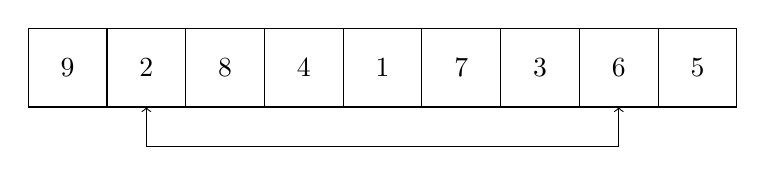
\begin{tikzpicture}
\draw (0, 0) -- (9, 0);
\draw (0, 1) -- (9, 1);

\foreach \i in {0, 1, 2, 3, 4, 5, 6, 7, 8, 9}
	\draw (\i, 0) -- (\i, 1);
	
\draw[<->] (1.5, 0) -- (1.5, -0.5) -- (7.5, -0.5) -- (7.5, 0);

\draw (0.5, 0.5) node{9};
\draw (1.5, 0.5) node{2};
\draw (2.5, 0.5) node{8};
\draw (3.5, 0.5) node{4};
\draw (4.5, 0.5) node{1};
\draw (5.5, 0.5) node{7};
\draw (6.5, 0.5) node{3};
\draw (7.5, 0.5) node{6};
\draw (8.5, 0.5) node{5};
\end{tikzpicture}

Především si povšimněme, že pořadí prvků 2 a~6 se nezmění vůči prvkům ležícím před prvkem 2 a~vůči prvkům ležícím za prvkem 6. Ke změnám inverzí tedy dochází jen mezi nimi:

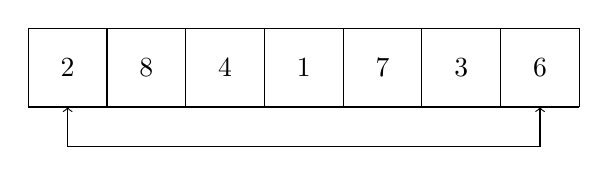
\begin{tikzpicture}
\draw (0, 0) -- (7, 0);
\draw (0, 1) -- (7, 1);

\foreach \i in {0, 1, 2, 3, 4, 5, 6, 7}
	\draw (\i, 0) -- (\i, 1);
	
\draw[<->] (0.5, 0) -- (0.5, -0.5) -- (6.5, -0.5) -- (6.5, 0);

\draw (0.5, 0.5) node{2};
\draw (1.5, 0.5) node{8};
\draw (2.5, 0.5) node{4};
\draw (3.5, 0.5) node{1};
\draw (4.5, 0.5) node{7};
\draw (5.5, 0.5) node{3};
\draw (6.5, 0.5) node{6};
\end{tikzpicture}

Dále si uvědomme, že čísla která jsou menší než číslo 2, jsou také menší než číslo 6. Záměnou prvku 2 za prvek 6 se tedy nezmění inverze s~prvky menšími než 2. Obdobně to platí pro prvky větší než 6. Počet inverzí s prvky ležící mimo aritmetický interval dvou prohazovaných čísel se proto nezmění. Stačí tedy uvažovat jen prvky ležící v~něm:


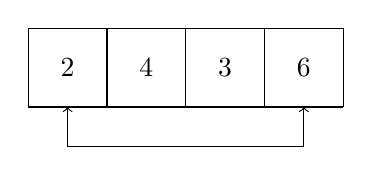
\begin{tikzpicture}
\draw (0, 0) -- (4, 0);
\draw (0, 1) -- (4, 1);

\foreach \i in {0, 1, 2, 3, 4}
	\draw (\i, 0) -- (\i, 1);
	
\draw[<->] (0.5, 0) -- (0.5, -0.5) -- (3.5, -0.5) -- (3.5, 0);

\draw (0.5, 0.5) node{2};
\draw (1.5, 0.5) node{4};
\draw (2.5, 0.5) node{3};
\draw (3.5, 0.5) node{6};
\end{tikzpicture}

Prozkoumejme změnu počtu inverzí s~některým ze zbývajících prvků, například s~prvkem 4. Před prohozením prvků 2 a~6 nejsou s~prvkem 4 žádné inverze, prohozením prvků 2 a~6 vzniknou inverze \((6, 4)\) a~\((4, 2)\). Povšimněme si, že takto vznikne nebo zanikne sudý počet inverzí - buď budeme mít konfiguraci \((2, ..., 4, ..., 6)\) bez inverzí nebo \((6, ..., 4, ..., 2)\) se dvěma inverzemi s~prvkem 4. Je to dáno tím, že prvek 4 leží aritmeticky i~pozičně mezi prvky 2 a 6 - důsledek naší předchozí úvahy o~prvcích mimo. Sudý počet inverzí vznikne nebo zanikne i~vůči ostatním prvkům. Plus vznikne nebo zanikne 1 inverze mezi prvky 2 a 6. Celkově se tedy počet inverzí změní o~lichý počet. 

\begin{fact}
Počet inverzí permutace se prohozením libovolných dvou prvků změní o~lichý počet. 
\end{fact}

To nám umožňuje rozdělit permutace na sudé a~liché:

\begin{fact}
Sudá permutace má sudý počet inverzí, lichá permutace má lichý počet inverzí. Prohozením dvou libovolných prvků se ze sudé permutace stane lichá a~naopak.
\end{fact}

Mějme \(n\) vektorů \(\vect{a}\), \(\vect{b}\), \(\vect{c}\), ... se složkami \(a_i\), \(b_j\), \(c_k\) atd. Pro každou permutaci utvoříme součin \(a_i \cdot b_j \cdot c_k \cdot ...\), kde indexy \(i, j, k, ...\) odpovídají prvkům permutace. Pokud se jedná o~lichou permutaci, tak součin násobíme \(-1\). Tedy pro permutaci \([1, 3, 2]\) budeme mít součin \(-a_1 \cdot b_3 \cdot c_2\). Udělejme součet takovýchto součinů pro všechny permutace. Pro \(n=3\) tedy získáme \(s = a_1 b_2 c_3 + a_2 b_3 c_1 + a_3 b_1 c_2 - a_1 b_3 c_2  - a_3 b_2 c_1 - a_2 b_1 c_3\).

Pokud bychom vektory uspořádali do matice, pak by uvedený součen součinů byl roven jejímu determinantu, tedy:

\begin{equation}
s = 
\begin{vmatrix}
a_1 & a_2 & a_3 \\
b_1 & b_2 & b_3 \\
c_1 & c_2 & c_3 \\
\end{vmatrix}
\end{equation}

Povšimněme si, co se stane, pokud by 2 vektory byli shodné, například pokud \(\vect{a} = \vect{b}\). Počítali-bychom determinant: 

\begin{equation}
s = 
\begin{vmatrix}
b_1 & b_2 & b_3 \\
b_1 & b_2 & b_3 \\
c_1 & c_2 & c_3 \\
\end{vmatrix}
\end{equation}

Získáme tak součet \(s = b_1 b_2 c_3 + b_2 b_3 c_1 + b_3 b_1 c_2 - b_1 b_3 c_2  - b_3 b_2 c_1 - b_2 b_1 c_3 = 0\). Vidíme, že součet je nulový, protože každý jeho člen se v~součtu objevuje jednou s~kladným znaménkem a~jendou se záporným znaménkem. To je důsledkem toho, že sme zavedli součet jako součet všech permutací. Například člen \(+b_1 b_2 c_3\) odpovídá sudé permutaci \(123\) a~člen \(-b_2 b_1 c_3\) liché permutaci \(213\). Protože tyto dvojice členů vzniknou tak, že prohodíme 2 prvky permutace, tak vždy jeden člen bude odpovídat sudé permutaci a~druhý liché permutaci. Proto budou mít vždy opačné zneménko. Obecně proto platí, že takto utvořený součet se dvěma stejnými vektory, tedy determinant matice se dvěma stejnými řádky, je nulový.

Zaveďme Levi-Civitův symbol \(\varepsilon_{ijk...}\):

\begin{fact}
Symbol \(\varepsilon_{ijk...}\) má v~\(n\)-rozměrném prostoru hodnotu \(n\) indexů \(i, j, k, ...\), které mohou nabývat hodnot \(1\) až \(n\). Tvoří-li indexy sudou permutací čísel \(1, 2, ..., n\), pak \(\varepsilon_{ijk...} = +1\). Tvoří-li indexy lichou permutaci, pak \(\varepsilon_{ijk...} = -1\). Netvoří-li indexy permutaci čísel \(1, 2, ..., n\), pak \(\varepsilon_{ijk...} = 0\). Tento případ nastává pokud 2 nebo více indexů je shodných.
\end{fact}

Ve třírozměrném prostoru tedy máme:

\begin{equation}
\begin{split}
\varepsilon_{123} = \varepsilon_{231} = \varepsilon_{312} = +1 \\
\varepsilon_{132} = \varepsilon_{213} = \varepsilon_{321} = -1 \\
\varepsilon_{iij} = \varepsilon_{iji} = \varepsilon_{jii} = 0
\end{split}
\end{equation}

Levi-Civitův symbol nám umožňuje zapsat součet součinů permutací složek \(n\) vektorů. Pro \(n = 3\) máme:

\begin{equation}
s = \sum_{i=1}^3 \sum_{j=1}^3 \sum_{k=1}^3 a_i b_j c_k \varepsilon_{ijk}
\end{equation}

Tuto rovnici můžeme rozepsat na 2:

\begin{equation}
\begin{split}
v_i = \sum_{j=1}^3 \sum_{k=1}^3 b_j c_k \varepsilon_{ijk} \\
s = \sum_{i=1}^3 a_i \cdot v_i
\end{split}
\end{equation}

Získáme tak vektor \(\vect{v}\).
Povšimněme si, že pokud zvolíme \(\vect{a} = \vect{b}\), pak \(s = \sum_{i=1}^3 \sum_{j=1}^3 \sum_{k=1}^3 b_i b_j c_k \varepsilon_{ijk} = 0\). To ale znamená, že \(s = \sum_{i=1}^3 b_i \cdot v_i = 0\), tedy vektor \(\vect{v}\) je kolmý na vektor \(\vect{b}\).

Obdobnou úvahou zjistíme, že vektor \(\vect{v}\) je kolmý na vektor \(\vect{c}\). Ve třírozměrném prostoru proto můžeme zavést tzv. vektorový součin, který utvoří vektor kolmý na 2 vektory:

\begin{equation}
\label{eq:vektorovy_soucin}
\begin{split}
\vect{v} = \vect{b} \times \vect{c} \\
v_i = \sum_{j=1}^3 \sum_{k=1}^3 b_j c_k \varepsilon_{ijk}
\end{split}
\end{equation}

Tuto rovnici můžeme rozepsat na jednotlivé složky uvědomíme-li si, že pouze 6 trojic indexů \(i, j, k\) odpovídá nenulovým \(\varepsilon_{ijk}\):

\begin{equation}
\begin{split}
\vect{v} = \vect{b} \times \vect{c} = \\
(b_2 c_3 - b_3 c_2, b_3 c_1 - b_1 c_3, b_1 c_2 - b_2 c_1) = \\
(b_y c_z - b_z c_y, b_z c_x - b_x c_z, b_x c_y - b_y c_x)
\end{split} 
\end{equation}

\section{Limita funkce}

V~metrickém prostoru \((M, d)\) pro \(\delta > 0\) definujme \(\delta\)-okolí prvku \(P \in M\) jako množinu bodů, jejichž vzdálenost od prvku \(P\) je menší než \(\delta\):

\begin{equation}
\forall \delta > 0, P \in M: U_{\delta}(P) = \{X \in M: d(X, P) < \delta\}
\end{equation}

Zaveďme také označení pro výlučné \(\delta\)-okolí prvku \(P\), tedy okolí bez vlastního bodu:

\begin{equation}
\overset{\circ}{U}_{\delta}(P) = U_{\delta}(P) \setminus P
\end{equation}

Pokud v~dalším textu neuvedeme jinak, tak za metrický prostor budeme považovat Euklidovský prostor. Budeme tedy používat metriku \eqref{eq:euklidovsky_prostor_metrika} i~v~případě, že ji bude nutné zavést uměle. V~Euklidovském prostoru představuje  \(\delta\)-okolí obecně hyperkouli okolo zvoleného bodu. V~jednorozměrném prostoru se jedná o~interval \(|x - x_0| < \delta\), ve dvojrozměrném prostoru o~kruh \((x - x_0)^2 + (y - y_0)^2 < \delta^2\) a~ve třírozměrném prostoru o~kouli \((x - x_0)^2 + (y - y_0)^2 + (z - z_0)^2 < \delta^2\).

Limitou funkce \(y = \lim_{P \to P_0} \mathrm{f}(P)\) rozumíme to, k~jaké funkční hodnotě se funkce blíží, pokud se její argumenty \(P\) blíží k~bodu \(P_0\). Přesná definice je následující. To, že funkce \(\mathrm{f}(P)\) má v~bodě \(P_0\) limitu \(y\) znamená, že pro každé kladné \(\varepsilon\) lze nalézt kladné \(\delta\) takové, že funkce má ve výlučném \(\delta\)-okolí bodu \(P_0\) hodnoty ležící v~\(\varepsilon\)-okolí bodu \(y\):

\begin{equation}
\forall \varepsilon > 0 \; \exists \delta > 0 \; \forall P \in \overset{\circ}{U}_{\delta}(P_0) \; \mathrm{f}(P) \in U_{\varepsilon}(y)
\end{equation}

Limitu tedy můžeme dokázat tak, že nalezneme funkci \(\delta(\varepsilon)\) splňující výše uvedené požadavky.

Na funkční hodnotě v~daném bodě nezáleží. Funkce nemusí být ani v~daném bodě definovaná. Funkce nemusí mít v~daném bodě limitu, pokud ji však má, tak je tato limita jednoznačně určená. Metrický prostor funkčních argumentů a~funkčních hodnot je obecně různý.

\subsection{Spojitost funkce}
\label{sec:spojitost_funkce}


Funkci nazveme spojitou v~daném bodě pokud je limita v~tomto bodě rovna funkční hodnotě. Tedy pokud v~daném bodě funkce limitů má, má v~něm i~funkční hodnotu a~limita je funkční hodnotě rovna. Tedy pokud

\begin{equation}
\lim_{P \to P_0} \mathrm{f}(P) = \mathrm{f}(P_0)
\end{equation}

Není-li funkce v daném bodě definovaná, ale je možné ji upravit tak, že se v~okolí bodu nezmění a~po úpravě bude spojitá, pak můžeme její limitu vypočítat jako hodnotu této upravené funkce. Příklad:

\begin{equation}
\lim_{x \to 0} \frac{2x}{x} = \lim_{x \to 0} 2 = 2
\end{equation}

\subsection{Příklad}

Dokažme \(\lim_{[x, y] \to [0, 2]} \frac{x^2 + x y}{x} = 2\).

Vyjádřeme vzdálenost od \(y\):

\begin{equation}
\begin{split}
|\mathrm{f}(P) - y| = \left|\frac{x^2 + x y}{x} - 2 \right| = \left|x + y - 2 \right| = \\
\left|dx + ( 2+ dy) - 2 \right| = \left|dx + dy\right| \leq 2 \cdot \delta
\end{split}
\end{equation}

Vidíme, že zvolíme-li \(\delta = \frac{\varepsilon}{2}\), pak pro \(\sqrt{x^2 + y^2} < \delta\) bude \(|\mathrm{f}(P) - y| = |x| < \varepsilon\).

\subsection{Limita složené funkce}

Pro limitu složených funkcí platí následující vztah. Přitom předpokládáme, že hodnota funkce g (bod \(Q_0\)) leží ve stejném metrickém prostoru jako argument funkce f (bod \(Q\)), tedy že se v obou případech používá stejná metrika.

\begin{equation}
\label{eq:limita_slozene_funkce}
\begin{split}
\lim_{P \to P_0} \mathrm{g}(P) = Q_0 \land \lim_{Q \to Q_0} \mathrm{f}(Q) = y \Rightarrow \lim_{P \to P_0} \mathrm{f}(\mathrm{g}(P)) = y
\end{split}
\end{equation}

Pokud je funkce \(f\) spojitá, tak její limitu můžeme nahradit její funkční hodnotou a~vztah se zjednodušší:

\begin{equation}
\label{eq:limita_spojite_slozene_funkce}
\begin{split}
\lim_{P \to P_0} \mathrm{f}(\mathrm{g}(P)) = \mathrm{f} \left( \lim_{P \to P_0} \mathrm{g}(P) \right)
\end{split}
\end{equation}

Obě dvě věty je třeba chápat jako implikace. Neexistence limit jednotlivých funkcí ještě neznemaná, že neexistuje limita složené funkce.

Přistupme k důkazu. Z~definice limit funkcí \(\mathrm{f}\) a~\(\mathrm{g}\) víme:

\begin{equation}
\begin{split}
\forall Q \in \overset{\circ}{U}_{\delta_f(\varepsilon_f)}(Q_0) \; \mathrm{f}(Q) \in U_{\varepsilon_f}(y) \\
\forall P \in \overset{\circ}{U}_{\delta_g(\varepsilon_g)}(P_0) \; \mathrm{g}(P) \in U_{\varepsilon_g}(Q_0)
\end{split}
\end{equation}

Uvědomíme-li si, že z~\(\varepsilon_g \leq \delta_f(\varepsilon_f)\) plyne

\begin{equation}
\overset{\circ}{U}_{\varepsilon_g}(Q_0) \subset \overset{\circ}{U}_{\delta_f(\varepsilon_f)}(Q_0)
\end{equation}

a~my můžeme první rovnici specializovat pokud zvolíme \(\varepsilon_g = \delta_f(\varepsilon_f)\):

\begin{equation}
\begin{split}
\forall Q \in \overset{\circ}{U}_{\delta_f(\varepsilon_f)}(Q_0) \; \mathrm{f}(Q) \in U_{\varepsilon_f}(y) \\
\forall Q \; Q \in \overset{\circ}{U}_{\delta_f(\varepsilon_f)}(Q_0) \Rightarrow \mathrm{f}(Q) \in U_{\varepsilon_f}(y)
\end{split}
\end{equation}

Rovnici jsme zapsali ve tvaru implikace, protože \(\forall A \in S \; p(A)\) je jen zjednodušený zápis pro \(\forall A \; A \in S \Rightarrow p(A)\). 

Dále pak můžeme dosadit \(Q = \mathrm{g}(P)\):

\begin{equation}
\forall P \; \mathrm{g}(P) \in \overset{\circ}{U}_{\delta_f(\varepsilon_f)}(Q_0) \Rightarrow \; \mathrm{f}(\mathrm{g}(P)) \in U_{\varepsilon_f}(y)
\end{equation}

Ve druhé rovnici také zavedeme substituci \(\varepsilon_g = \delta_f(\varepsilon_f)\):

\begin{equation}
\begin{split}
\forall P \in \overset{\circ}{U}_{\delta_g(\delta_f(\varepsilon_f))}(P_0) \; \mathrm{g}(P) \in U_{\delta_f(\varepsilon_f)}(Q_0) \\
\forall P \; P \in \overset{\circ}{U}_{\delta_g(\delta_f(\varepsilon_f))}(P_0) \Rightarrow \mathrm{g}(P) \in U_{\delta_f(\varepsilon_f)}(Q_0)
\end{split}
\end{equation}

Obě rovnice jsou ve tvaru 2 implikací a~je možné využít transitivitu implikací. Získáme tak rovnici:

\begin{equation}
\begin{split}
\forall P \; P \in \overset{\circ}{U}_{\delta_g(\delta_f(\varepsilon_f))}(P_0) \Rightarrow \mathrm{f}(\mathrm{g}(P)) \in U_{\varepsilon_f}(y) \\
\forall P \in \overset{\circ}{U}_{\delta_g(\delta_f(\varepsilon_f))}(P_0) \; \mathrm{f}(\mathrm{g}(P)) \in U_{\varepsilon_f}(y)
\end{split}
\end{equation}

Tím je dokázán vztah pro limitu složené funkce.

\subsection{Zůžení limity}

Mějme funkci dvou proměnných \(\mathrm{g}(a, b)\). Pak existují-li limity na levé straně následujících rovností, pak rovnosti platí:

\begin{equation}
\label{eq:zuzeni_limity_fixace}
\lim_{a \to a_0} \lim_{b \to b_0} \mathrm{g}(a, b) = \lim_{[a, b] \to [a_0, b_0]} \mathrm{g}(a, b) = \lim_{a \to a_0} \mathrm{g}(a, b_0) = \lim_{b \to b_0} \mathrm{g}(a_0, b)
\end{equation}

\begin{equation}
\label{eq:zuzeni_limity_stejne_promenne}
\lim_{a \to x_0} \lim_{b \to x_0} \mathrm{g}(a, b) = \lim_{[a, b] \to [x_0, x_0]} \mathrm{g}(a, b) = \lim_{x \to x_0} \mathrm{g}(x, x)
\end{equation}

Důkaz je zřejmý, okolí bodů u~limit vpravo je podmnožinou okolí bodů u~limit vlevo.

\subsection{Základní limity}

Níže jsou uvedeny základní limity. Předpokládáme při tom, že limity podvýrazů existují. Vztahy jsou odvozeny ze vztahu~\eqref{eq:limita_spojite_slozene_funkce}.

\begin{equation}
\lim_{P \to P_0} \left(\mathrm{f}(P) \pm \mathrm{g}(P) \right) = \lim_{P \to P_0} \mathrm{f}(P) \pm \lim_{P \to P_0} \mathrm{g}(P)
\end{equation}

\begin{equation}
\lim_{P \to P_0} \left(\mathrm{f}(P) \cdot \mathrm{g}(P) \right) = \lim_{P \to P_0} \mathrm{f}(P) \cdot \lim_{P \to P_0} \mathrm{g}(P)
\end{equation}

\begin{equation}
\lim_{P \to P_0} \frac{\mathrm{f}(P)}{\mathrm{g}(P)} = \frac{\lim_{P \to P_0} \mathrm{f}(P)}{\lim_{P \to P_0} \mathrm{g}(P)}; \lim_{P \to P_0} \mathrm{g}(P) \neq 0
\end{equation}

\begin{equation}
\lim_{P \to P_0} \left(\mathrm{f}(P)\right)^n = \left(\lim_{P \to P_0} \mathrm{f}(P)\right)^n; n > 0
\end{equation}

\begin{equation}
\lim_{P \to P_0} \left(\mathrm{f}(P)\right)^{\mathrm{g}(P)} = \left(\lim_{P \to P_0} \mathrm{f}(P)\right)^{\lim_{P \to P_0} \mathrm{g}(P)}; \lim_{P \to P_0} \mathrm{f}(P) > 0
\end{equation}

\section{Derivace}

Derivací funkce rozumíme poměr změny funkční hodnoty vůči změne jejího parametru:

\begin{equation}
\label{eq:definice_derivace}
\begin{split}
z =\mathrm{f}(x) \\
\frac{\mathrm{d}z}{\mathrm{d}x} = \lim_{\mathrm{d}x \to 0} \frac{\mathrm{f}(x + \mathrm{d}x) - \mathrm{f}(x)}{\mathrm{d}x}
\end{split}
\end{equation}

Máme-li funkci více parametrů, pak ostatní parametry považujeme za konstantní. Takovou derivaci nazýváme parciální. Samozřejmě je možné vypočítat parciální derivace vůči všem parametrům:

\begin{equation}
\begin{split}
z =\mathrm{f}(x, y) \\
\frac{\partial z}{\partial x} = \lim_{\mathrm{d}x \to 0} \frac{\mathrm{f}(x + \mathrm{d}x, y) - \mathrm{f}(x, y)}{\mathrm{d}x} \\
\frac{\partial z}{\partial y} = \lim_{\mathrm{d}y \to 0} \frac{\mathrm{f}(x, y + \mathrm{d}y) - \mathrm{f}(x, y)}{\mathrm{d}y}
\end{split}
\end{equation}

Je nutné mít na paměti, že \(\frac{\mathrm{d}z}{\mathrm{d}x}\) ani \(\frac{\partial z}{\partial x}\) nejsou podíly nebo zlomky, jedná se o symboly pro derivace. Později sice uvidíme, že například derivace složené funkce vypadá jako krácení zlomků, ale ve skutečnosti je to opět jen symbolika zápisu.

\begin{figure}
\begin{center}
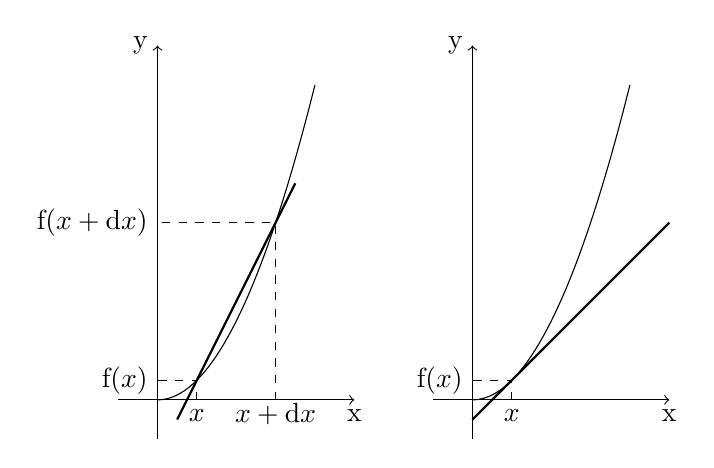
\begin{tikzpicture}
// Secna
\draw[->] (-0.5, 0) -- (2.5, 0);
\draw (2.5, 0) node[anchor=north]{x};

\draw[->] (0, -0.5) -- (0, 4.5);
\draw (0, 4.5) node[anchor=east]{y};

\draw[domain=0:2, smooth, variable = \x] plot ({\x}, {\x * \x});

\draw[thick] (0.25, -0.25) -- (1.75, 2.75); 

\draw[dashed] (0.5, 0) -- (0.5, 0.25) -- (0, 0.25);
\draw[dashed] (1.5, 0) -- (1.5, 2.25) -- (0, 2.25);

\draw (0.5, 0) node[anchor=north]{\(x\)};
\draw (1.5, 0.08) node[anchor=north]{\(x + \mathrm{d}x\)};

\draw (0, 0.25) node[anchor=east]{\(\mathrm{f}(x)\)};
\draw (0, 2.25) node[anchor=east]{\(\mathrm{f}(x + \mathrm{d}x)\)};

// Tecna
\draw[->] (3.5, 0) -- (6.5, 0);
\draw (6.5, 0) node[anchor=north]{x};

\draw[->] (4, -0.5) -- (4, 4.5);
\draw (4, 4.5) node[anchor=east]{y};

\draw[domain=0:2, smooth, variable = \x] plot ({\x + 4}, {\x * \x});

\draw[thick] (4.0, -0.25) -- (6.5, 2.25); 

\draw[dashed] (4.5, 0) -- (4.5, 0.25) -- (4, 0.25);

\draw (4.5, 0) node[anchor=north]{\(x\)};
\draw (4, 0.25) node[anchor=east]{\(\mathrm{f}(x)\)};

\end{tikzpicture}
\caption{Derivace funkce}
\end{center}
\label{img:derivace}
\end{figure}

Na obrázku \ref{img:derivace} je vidět grafický význam derivace. Přímka procházející body \([x, \mathrm{f}(x)]\) a~\([x + \mathrm{d}x, \mathrm{f}(x + \mathrm{d}x)]\) tvoří sečnu funkce \(\mathrm{f}\). Pokud \(\mathrm{d}x \to 0\), pak se sečna bude blížit tečně. Derivace proto představuje směrnici tečny v~daném bodě.

\subsection{Derivace složené funkce jedné proměnné}

Mějme složenou funkci

\begin{equation}
y = \mathrm{f}(\mathrm{g}(x))
\end{equation}

a~chtějme vypočítat její derivaci. Derivaci můžeme vypočítat podle definice~\eqref{eq:definice_derivace}:

\begin{equation}
\label{eq:derivace_slozene_funkce_vypocet}
\begin{split}
\frac{\mathrm{d}y}{\mathrm{d}x} = \lim_{\mathrm{d}x \to 0} \frac{\mathrm{f}(\mathrm{g}(x + \mathrm{d}x)) - \mathrm{f}(\mathrm{g}(x))}{\mathrm{d}x} = \\
\lim_{\mathrm{d}x \to 0} \frac{\mathrm{f}(\mathrm{g}(x + \mathrm{d}x)) - \mathrm{f}(\mathrm{g}(x))}{\mathrm{d}x} \cdot \frac{\mathrm{g}(x + \mathrm{d}x) - \mathrm{g}(x)}{\mathrm{g}(x + \mathrm{d}x) - \mathrm{g}(x)} = \\
\lim_{\mathrm{d}x \to 0} \frac{\mathrm{f}(\mathrm{g}(x) + \mathrm{g}(x + \mathrm{d}x) - \mathrm{g}(x)) - \mathrm{f}(\mathrm{g}(x))}{\mathrm{g}(x + \mathrm{d}x) - \mathrm{g}(x)} \cdot \frac{\mathrm{g}(x + \mathrm{d}x) - \mathrm{g}(x)}{\mathrm{d}x} = \\
\lim_{\mathrm{d}x \to 0} \frac{\mathrm{f}(\mathrm{g}(x) + \mathrm{g}(x + \mathrm{d}x) - \mathrm{g}(x)) - \mathrm{f}(\mathrm{g}(x))}{\mathrm{g}(x + \mathrm{d}x) - \mathrm{g}(x)} \cdot \lim_{\mathrm{d}x \to 0} \frac{\mathrm{g}(x + \mathrm{d}x) - \mathrm{g}(x)}{\mathrm{d}x} = \\
\lim_{\mathrm{d}g \to 0} \frac{\mathrm{f}(\mathrm{g}(x) + \mathrm{d}g) - \mathrm{f}(\mathrm{g}(x))}{\mathrm{d}g} \cdot \lim_{\mathrm{d}x \to 0} \frac{\mathrm{g}(x + \mathrm{d}x) - \mathrm{g}(x)}{\mathrm{d}x} = \\
\frac{\mathrm{df}}{\mathrm{d}g}(\mathrm{g}(x)) \cdot \frac{\mathrm{dg}}{\mathrm{d}x}
\end{split}
\end{equation}

Několikrát jsme využili vztah pro limitu složené funkce~\eqref{eq:limita_slozene_funkce}. Zapišme odvozený vztah ještě jednou, protože se jedná o~velmi důležitý vztah:

\begin{equation}
\frac{\mathrm{d}y}{\mathrm{d}x} = \frac{\mathrm{d}}{\mathrm{d}x}\mathrm{f}(\mathrm{g}(x)) = \frac{\mathrm{df}}{\mathrm{d}g}(\mathrm{g}(x)) \cdot \frac{\mathrm{dg}}{\mathrm{d}x}
\end{equation}

Derivaci složené funkce \(\mathrm{f}(\mathrm{g}(x))\) tedy vypočítáme tak, že vypočítáme derivaci vnější funkce \(\mathrm{f}\) vůči jejímu parametru \(g\) vyhodnocenou v~bodě \(\mathrm{g}(x)\) a~vynásobíme ji derivací vnitřní funkce \(\mathrm{g}\). Vnitřní funkce je vyhodnocena v~bodě \(x\), ale to není nutné explicitně zapisovat.

\subsection{Derivace složené funkce více proměnných}

Mějme složenou funkci 2 proměnných:

\begin{equation}
y = \mathrm{f}(\mathrm{g}(x), \mathrm{h}(x))
\end{equation}

Její derivace je určena vztahem

\begin{equation}
\frac{\partial y}{\partial x} = \lim_{\mathrm{d}x \to 0} \frac{\mathrm{f}(\mathrm{g}(x + \mathrm{d}x), \mathrm{h}(x + \mathrm{d}x)) - \mathrm{f}(\mathrm{g}(x), \mathrm{h}(x))}{\mathrm{d}x}
\end{equation}

Nyní využijeme triku, který je v~této knize využit několikrát. Jednou z~možností, jak se z~bodu \(A\) dostat do bodu \(B\) je podél souřadnicových os. Nejdříve podél osy \(x\), pak podél osy \(y\) atd. V~našem případě to znamená:


\begin{equation}
\begin{split}
\frac{\partial y}{\partial x} = \lim_{\mathrm{d}x \to 0} \frac{\mathrm{f}(\mathrm{g}(x + \mathrm{d}x), \mathrm{h}(x + \mathrm{d}x)) - \mathrm{f}(\mathrm{g}(x), \mathrm{h}(x + \mathrm{d}x))}{\mathrm{d}x} + \\
\lim_{\mathrm{d}x \to 0} \frac{\mathrm{f}(\mathrm{g}(x), \mathrm{h}(x + \mathrm{d}x)) - \mathrm{f}(\mathrm{g}(x), \mathrm{h}(x))}{\mathrm{d}x} = \\
\lim_{\varepsilon \to 0} \lim_{\mathrm{d}x \to 0} \frac{\mathrm{f}(\mathrm{g}(x + \mathrm{d}x), \mathrm{h}(x + \varepsilon)) - \mathrm{f}(\mathrm{g}(x), \mathrm{h}(x + \varepsilon))}{\mathrm{d}x} + \\
\lim_{\mathrm{d}x \to 0} \frac{\mathrm{f}(\mathrm{g}(x), \mathrm{h}(x + \mathrm{d}x)) - \mathrm{f}(\mathrm{g}(x), \mathrm{h}(x))}{\mathrm{d}x} = \\
\lim_{\varepsilon \to 0} \frac{\partial \mathrm{f}}{\partial g}(\mathrm{g}(x), \mathrm{h}(x + \varepsilon)) \cdot \frac{\partial \mathrm{g}}{\partial x} +
\frac{\partial \mathrm{f}}{\partial h}(\mathrm{g}(x), \mathrm{h}(x)) \cdot \frac{\partial \mathrm{h}}{\partial x} = \\
\frac{\partial \mathrm{f}}{\partial g}(\mathrm{g}(x), \mathrm{h}(x)) \cdot \frac{\partial \mathrm{g}}{\partial x} +
\frac{\partial \mathrm{f}}{\partial h}(\mathrm{g}(x), \mathrm{h}(x)) \cdot \frac{\partial \mathrm{h}}{\partial x}
\end{split}
\end{equation}

Nejdříve jsme k~výrazu přičetli a~odečetli člen \(\mathrm{f}(\mathrm{g}(x), \mathrm{h}(x + \mathrm{d}x))\) a~limitu rozdělili na dvě. Dále jsme jeden člen \(d_x\) nahradili nově zavedeným členem \(\varepsilon\). Využili jsme při tom vztahu \eqref{eq:zuzeni_limity_stejne_promenne}.
Nakonec jsme limity nahradili derivacemi podle vztahu~\eqref{eq:derivace_slozene_funkce_vypocet}, jen funkci dvou proměnných s~jednou proměnnou konstantní chápeme jako funkci jedné proměnné.

Tento vztah lze zobecnit na složenou funkci libovolného počtu proměnných:

\begin{equation}
\frac{\partial}{\partial x} \mathrm{f} (\mathrm{g}_1(x, y, ...), \mathrm{g}_2(x, y, ...), ..., \mathrm{g}_n(x, y, ...)) = \sum_{i=1}^n \frac{\partial \mathrm{f}}{\partial g_i}(\mathrm{g}(x)) \cdot \frac{\partial \mathrm{g}_i}{\partial x}
\end{equation}

\subsection{Derivace inverzní funkce}

Mějme navzájem inverzní funkce \(\mathrm{f}(x)\) a~\(\mathrm{g}(x)\). Pak pro ně musí platit:

\begin{equation}
\mathrm{f}(\mathrm{g}(x)) = x
\end{equation}

Derivace stejných funkcí musí být stejná, to vyplývá z~definice derivace. To znamená, že můžeme zderivovat obě strany rovnice, protože rovnost zůstane zachována. Získáme tak rovnici:

\begin{equation}
\label{eq:derivace_inverzni_funkce}
\begin{split}
\frac{\mathrm{df}}{\mathrm{d}x}(\mathrm{g}(x)) \cdot \frac{\mathrm{dg}}{\mathrm{d}x} = 1 \\
\frac{\mathrm{dg}}{\mathrm{d}x} = \frac{1}{\frac{\mathrm{df}}{\mathrm{d}x}(\mathrm{g}(x))}
\end{split}
\end{equation}

\subsection{Tabulka derivací}

Vypočítejme derivace různých funkcí. Začněme derivací konstantní funkce, přesněji funkce nezávislé na proměnné, podle které derivujeme:

\begin{equation}
\frac{\mathrm{d}k}{\mathrm{d}x} = \lim_{dx \to 0} \frac{k - k}{dx} = \lim_{dx \to 0} 0 = 0¨
\end{equation}

Pokračujme derivací součtu a~rozdílu funkcí. K~tomu budeme potřebovat derivaci přímé úměry:

\begin{equation}
\frac{\mathrm{d}}{\mathrm{d}x} kx = \lim_{dx \to 0} \frac{k \cdot (x + dx) - kx}{dx} = \lim_{dx \to 0} k = k
\end{equation}

Derivaci součtu a~rozdílu funkcí vypočítáme jako derivaci složené funkce. Označme vnější funkci \(\mathrm{s}(f, g) = f \pm g\). Ta je vůči svým parametrům \(f\) a~\(g\) přímo úměrná s~koeficientem 1 pro parametr \(f\) a \(\pm1\) pro parametr \(g\), tedy \(\frac{\mathrm{ds}}{\mathrm{d}f} = 1\) a~\(\frac{\mathrm{ds}}{\mathrm{d}g} = \pm1\):

\begin{equation}
\frac{\mathrm{d}}{\mathrm{d}x} (\mathrm{f}(x) \pm \mathrm{g}(x)) = \frac{\mathrm{d}}{\mathrm{d}x} \mathrm{s}(\mathrm{f}(x), \mathrm{g}(x)) = \frac{\mathrm{ds}}{\mathrm{d}f} \cdot \frac{\mathrm{df}}{\mathrm{d}x} + \frac{\mathrm{ds}}{\mathrm{d}g} \cdot \frac{\mathrm{dg}}{\mathrm{d}x} = \frac{\mathrm{df}}{\mathrm{d}x} \pm \frac{\mathrm{dg}}{\mathrm{d}x}
\end{equation}

Derivaci součinu funkcí vypočítáme opět jako derivaci složené funkce. Označme vnější funkci \(\mathrm{s}(f, g) = f \cdot g\). Ta je vůči svým parametrům \(f\) a~\(g\) přímo úměrná s~koeficientem druhého parametru, tedy \(\frac{\mathrm{ds}}{\mathrm{d}f} = g\) a~\(\frac{\mathrm{ds}}{\mathrm{d}g} = f\):

\begin{equation}
\begin{split}
\frac{\mathrm{d}}{\mathrm{d}x} (\mathrm{f}(x) \cdot \mathrm{g}(x)) = \frac{\mathrm{d}}{\mathrm{d}x} \mathrm{s}({f}(x), \mathrm{g}(x)) = \\
\frac{\mathrm{ds}}{\mathrm{d}f} (\mathrm{f}(x), \mathrm{g}(x)) \cdot \frac{\mathrm{df}}{\mathrm{d}x} + \frac{\mathrm{ds}}{\mathrm{d}g}(\mathrm{f}(x), \mathrm{g}(x)) \cdot \frac{\mathrm{dg}}{\mathrm{d}x} = \\
\mathrm{g}(x) \cdot \frac{\mathrm{df}}{\mathrm{d}x} + \mathrm{f}(x) \cdot \frac{\mathrm{dg}}{\mathrm{d}x}
\end{split}
\end{equation}

Pokud je jeden ze součinitelů nezávislý na proměnné, vůči které se derivuje, pak se vztah zjednodušší:

\begin{equation}
\begin{split}
\frac{\mathrm{d}}{\mathrm{d}x} (k \cdot \mathrm{f}(x)) = k \cdot \frac{\mathrm{df}}{\mathrm{d}x}
\end{split}
\end{equation}

Pro výpočet derivace podílu funkcí budeme znát derivaci inverzní funkce \(\frac{1}{x}\):

\begin{equation}
\begin{split}
\frac{\mathrm{d}}{\mathrm{d}x} \frac{1}{x} = \lim_{dx \to 0} \frac{\frac{1}{x + dx} - \frac{1}{x}}{dx} = \\
\lim_{dx \to 0} \frac{\frac{x - x - dx}{(x + dx) \cdot x}}{dx} = \lim_{dx \to 0} \frac{\frac{-dx}{(x + dx) \cdot x}}{dx} = \\
\lim_{dx \to 0} \frac{-1}{(x + dx) \cdot x} = -\frac{1}{x^2}
\end{split}
\end{equation}

Derivaci podílu funkcí vypočítáme opět jako derivaci složené funkce. Označme vnější funkci \(\mathrm{s}(f, g) = \frac{f}{g}\). Pak \(\frac{\mathrm{ds}}{\mathrm{d}f} = \frac{1}{g}\) a~\(\frac{\mathrm{ds}}{\mathrm{d}g} = -\frac{f}{g^2}\):

\begin{equation}
\begin{split}
\frac{\mathrm{d}}{\mathrm{d}x} \frac{\mathrm{f}(x)}{\mathrm{g}(x)} = \frac{\mathrm{d}}{\mathrm{d}x} \mathrm{s}({f}(x), \mathrm{g}(x)) = \\
\frac{\mathrm{ds}}{\mathrm{d}f} (\mathrm{f}(x), \mathrm{g}(x)) \cdot \frac{\mathrm{df}}{\mathrm{d}x} + \frac{\mathrm{ds}}{\mathrm{d}g}(\mathrm{f}(x), \mathrm{g}(x)) \cdot \frac{\mathrm{dg}}{\mathrm{d}x} = \\
\frac{1}{\mathrm{g}(x)} \cdot \frac{\mathrm{df}}{\mathrm{d}x} -\frac{\mathrm{f}(x)}{\mathrm{g}^2(x)} \cdot \frac{\mathrm{dg}}{\mathrm{d}x} = \\
\frac{\frac{\mathrm{df}}{\mathrm{d}x} \cdot \mathrm{g}(x) - \mathrm{f}(x) \cdot \frac{\mathrm{dg}}{\mathrm{d}x}}{\mathrm{g}^2(x)}
\end{split}
\end{equation}

Dále dokážeme matematickou indukcí vztah

\begin{equation}
\label{eq:derivace_mocniny_n}
\frac{\mathrm{d}}{\mathrm{d}x} x^n = n \cdot x^{n-1}; n \in \mathbb{N}
\end{equation}

Pro \(n = 1\) získáme vztah 

\begin{equation}
\frac{\mathrm{d}}{\mathrm{d}x} x = 1
\end{equation}

který jsme už dokázaly. Dále, pokud platí 

\begin{equation}
\frac{\mathrm{d}}{\mathrm{d}x} x^{n-1} = (n - 1) \cdot x^{n-2}; n \geq 2
\end{equation}

pak

\begin{equation}
\begin{split}
\frac{\mathrm{d}}{\mathrm{d}x} x^n = \frac{\mathrm{d}}{\mathrm{d}x} (x \cdot x^{n-1}) = x^{n-1} \cdot \frac{\mathrm{d}}{\mathrm{d}x} x + x \cdot \frac{\mathrm{d}}{\mathrm{d}x} x^{n-1} = \\
x^{n-1} + x \cdot (n - 1) \cdot x^{n-2} = x^{n-1} + (n - 1) \cdot x^{n-1} = n \cdot x^{n-1}
\end{split}
\end{equation}

a~proto vztah \eqref{eq:derivace_mocniny_n} platí pro všechna přirozená čísla.

\subsubsection{Derivace exponenciální funkce}

Mějme funkci \(y = a^x\) pro \(a > 0\). Její derivace je:

\begin{equation}
\begin{split}
\frac{\mathrm{d}y}{\mathrm{d}x} = \frac{\mathrm{d}}{\mathrm{d}x} a^x = \lim_{dx \to 0} \frac{a^{x+dx} - a^x}{dx} = \lim_{dx \to 0} \frac{a^x \cdot a^{dx} - a^x}{dx} = \\
a^x \cdot \lim_{dx \to 0} \frac{a^{dx} - 1}{dx} = y \cdot \frac{\mathrm{d}y}{\mathrm{d}x}(0)
\end{split}
\end{equation}

Vidíme, že derivace funkce \(a^x\) je rovna \(a^x\) násobené derivací v~bodě \(x = 0\).

\begin{figure}
\begin{center}
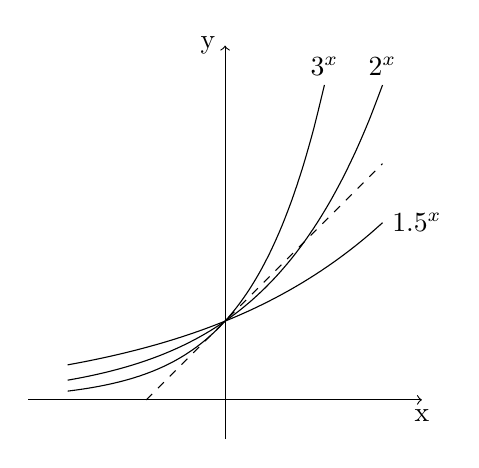
\begin{tikzpicture}
\draw[->] (-2.5, 0) -- (2.5, 0);
\draw (2.5, 0) node[anchor=north]{x};

\draw[->] (0, -0.5) -- (0, 4.5);
\draw (0, 4.5) node[anchor=east]{y};

\draw[domain=-2:2, smooth, variable = \x] plot ({\x}, {pow(1.5, \x)}) node[anchor=west]{\(1.5^x\)};
\draw[domain=-2:2, smooth, variable = \x] plot ({\x}, {pow(2, \x)}) node[anchor=south]{\(2^x\)};
\draw[domain=-2:1.2619, smooth, variable = \x] plot ({\x}, {pow(3, \x)}) node[anchor=south]{\(3^x\)};

\draw[dashed] (-1, 0) -- (2, 3);

\end{tikzpicture}
\caption{Derivace exponenciální funkce}
\end{center}
\label{img:derivace_exponencialni_funkce}
\end{figure}

Na obrázku~\ref{img:derivace_exponencialni_funkce} vidíme několik různých exponenciálních funkcí, všechny procházejí budem \([0, 1]\) protože \(a^0 = 1\). Na obrázku je také čárkovaně zakreslena přímka odpovídající v~tomto bodě tečně funkce s~derivací 1. Vidíme, že existuje základ mocniny, pro kterou bude tato přímka tečnou a~že leží mezi čísly 2 a~3. Tento základ nazveme Eulerovým číslem po slavném matematikovy a~označíme jej \(e\). Pro Eulerovo číslo tedy musí platit:

\begin{equation}
\lim_{dx \to 0} \frac{e^{dx} - 1}{dx} = 1
\end{equation}

Z~něj můžeme Eulerovo číslo vyjádřit:

\begin{equation}
\begin{split}
\lim_{dx \to 0} e^{dx} - 1 = \lim_{dx \to 0} dx \\
\lim_{dx \to 0} e^{dx} = \lim_{dx \to 0} (1 + dx) \\
e = \lim_{dx \to 0} \sqrt[dx]{1 + dx}
\end{split}
\end{equation}

Zavedeme-li substituci \(dx = \frac{1}{n}\), pak dostaneme známý vztah pro výpočet Eulerova čísla:

\begin{equation}
e = \lim_{n \to \infty} \left(1 + \frac{1}{n}\right)^n
\end{equation}

Uvedená limita znamená, že \(n\) roste nade všechny meze, přesnou definici zde nebudeme uvádět. Je zřejmé, že pokud \(n \to \infty\), pak \(dx \to 0\). Například pro \(n = 2^{66}\) dostaneme \(e \approx 2.718281828459045235\).

Proto platí:

\begin{equation}
\frac{\mathrm{d}}{\mathrm{d}x} e^x = e^x
\end{equation}

Inverzní funkcí je přirozený logaritmus \(\ln x\). Proto platí:

\begin{equation}
\ln e^x = x
\end{equation}

\begin{equation}
e^{\ln x} = x; x > 0
\end{equation}

Obecnou exponenciální funkci proto můžeme zapsat

\begin{equation}
a^x = e^{\ln a^x} = e^{x \cdot \ln a}; a > 0
\end{equation}

a~proto

\begin{equation}
\frac{\mathrm{d}}{\mathrm{d}x} a^x = \frac{\mathrm{d}}{\mathrm{d}x} e^{x \cdot \ln a} = e^{x \cdot \ln a} \cdot \ln a = \ln a \cdot a^x
\end{equation}

\subsubsection{Derivace přirozeného logaritmu}

Vyjdeme z~identity

\begin{equation}
e^{\ln x} = x; x > 0
\end{equation}

a~použitím vztahu~\eqref{eq:derivace_inverzni_funkce} získáme

\begin{equation}
\frac{\mathrm{d}}{\mathrm{d}x} \ln x = \frac{1}{e^{\ln x}} = \frac{1}{x}; x > 0
\end{equation}

\subsubsection{Derivace reálné mocniny}

Dříve jsme dokázali vztah \(\frac{\mathrm{d}}{\mathrm{d}x} x^n = n \cdot x^{n-1}\) pro \(x \in \mathbb{R}\) a~\(n \in \mathbb{N}\). Nyní dokážeme, že tento vztah platí i~pro reálné exponenty. Protože platí

\begin{equation}
x^r = e^{\ln x^r} = e^{r \cdot \ln x}; x \in \mathbb{R}^+, r \in \mathbb{R}
\end{equation}

tak proto platí

\begin{equation}
\frac{\mathrm{d}}{\mathrm{d}x} x^r = \frac{\mathrm{d}}{\mathrm{d}x} e^{r \cdot \ln x} = e^{r \cdot \ln x} \cdot r \cdot \frac{1}{x} = x^r \cdot r \cdot \frac{1}{x} = r \cdot x^{r-1}; x > 0
\end{equation}


\subsection{Jak derivovat}

S~využitím tabulky derivací primitivních funkcí a~pravidlem pro derivování složených funkcí lze derivovat čistě mechanicky "zeshora dolů". Zkusme zderivovat například:

\begin{equation}
\frac{\mathrm{d}}{\mathrm{d}x} \left(e^{2x+1} + 3x \right)^3 = ...
\end{equation}

Nejvýše postavenou funkcí je \(a^3\) s~\(a = e^{2x+1} + 3x\). Je to ta funkce, kterou bychom při vyčíslování výrazu vypočítali až nakonec. Víme, že derivace \(x^3\) je \(3 x^2\) a~využijeme pravidlo pro derivování složené funkce:

\begin{equation}
... = 3 \cdot \left(e^{2x+1} + 3x \right)^2 \cdot \frac{\mathrm{d}}{\mathrm{d}x} \left(e^{2x+1} + 3x \right) = ...
\end{equation}

Využijeme pravidlo pro derivaci součtu:

\begin{equation}
... = 3 \cdot \left(e^{2x+1} + 3x \right)^2 \cdot \left(\frac{\mathrm{d}}{\mathrm{d}x} e^{2x+1} + \frac{\mathrm{d}}{\mathrm{d}x} 3x \right) = ...
\end{equation}

První člen je \(e^b\) kde \(b = 2x + 1\), ten opět zderivujeme jako složenou funkci. Na druhý člen využijeme pravidlo pro derivaci součinu funkcí. Jedná se o~speciální případ, kdy jedna funkce je konstantní:

\begin{equation}
... = 3 \cdot \left(e^{2x+1} + 3x \right)^2 \cdot \left(e^{2x+1} \cdot \frac{\mathrm{d}}{\mathrm{d}x} \left(2x+1\right) + 3 \cdot \frac{\mathrm{d}}{\mathrm{d}x} x \right) = ...
\end{equation}

Na první člen použijeme pravidlo pro derivaci součtu. Derivace druhého členu \(x\) je 1:

\begin{equation}
... = 3 \cdot \left(e^{2x+1} + 3x \right)^2 \cdot \left(e^{2x+1} \cdot \left(\frac{\mathrm{d}}{\mathrm{d}x} 2x + \frac{\mathrm{d}}{\mathrm{d}x} 1\right) + 3 \right) = ...
\end{equation}

Derivace členu \(2x\) je 2, už ji nebudu znovu rozepisovat na derivaci součinu. Derivace konstanty 1 je 0. Získáme tak výsledek:

\begin{equation}
... = 3 \cdot \left(e^{2x+1} + 3x \right)^2 \cdot \left(2 e^{2x+1} + 3 \right)
\end{equation}

Tento postup je obecný a~s~trochou cviku lze derivace jednodušších výrazů psát napřímo bez rozepisování mezikroků. 

\subsection{Vícenásobná derivace}

Derivací funkce je funkce, kterou můžeme opět derivovat. Máme-li funkci více proměnných, pak můžeme derivotat podle stejné nebo podle jiné proměnné.

Mějme například funkci \(\mathrm{f}(x) = x^3 y^2\). Pak \(\frac{\partial \mathrm{f}}{\partial x} = 3 x^2 y^2\). Tuto první derivaci můžeme opět derivovat podle \(x\) a~získáme \(\frac{\partial^2 \mathrm{f}}{\partial x^2} = 6 x y^2\). Nebo podle \(y\) a~získáme \(\frac{\partial^2 \mathrm{f}}{\partial xy} = 6 x^2 y\).
Funkci \(f\) můžeme také derivovat podle \(y\) a~získáme \(\frac{\partial \mathrm{f}}{\partial y} = 2 x^3 y\). Derivujeme-li tuto derivaci podle \(x\), tak získáme \(\frac{\partial^2 \mathrm{f}}{\partial yx} = 6 x^2 y\).

Povšimněme si, že \(\frac{\partial^2 \mathrm{f}}{\partial xy} = \frac{\partial^2 \mathrm{f}}{\partial yx}\). To, že nezáleží na pořadí derivování, nyní dokážeme obecně:

\begin{equation}
\begin{split}
\frac{\partial^2 \mathrm{f}}{\partial yx} = \\
\lim_{dx \to 0} \frac{\lim_{dy \to 0} \frac{\mathrm{f}(x+dx, y+dy) - \mathrm{f}(x+dx, y)}{dy} - \lim_{dy \to 0} \frac{\mathrm{f}(x, y+dy) - \mathrm{f}(x, y)}{dy}}{dx} = \\
\lim_{dx \to 0, dy \to 0} \frac{\mathrm{f}(x+dx, y+dy) - \mathrm{f}(x+dx, y) - \mathrm{f}(x, y+dy) + \mathrm{f}(x, y)}{dx \cdot dy} = \\
\lim_{dx \to 0} \frac{\lim_{dy \to 0} \frac{\mathrm{f}(x+dx, y+dy) - \mathrm{f}(x, y+dy)}{dx} - \lim_{dy \to 0} \frac{\mathrm{f}(x+dx, y) - \mathrm{f}(x, y)}{dx}}{dy} = \\
\frac{\partial^2 \mathrm{f}}{\partial xy}
\end{split}
\end{equation}


\section{Objekty v~prostoru}

Souřadné systémy nám umožňují popisovat objekty v~prostoru. Nyní si ukážeme, jak je to možné.

\subsection{Bod}

Začněme nejjednodušším objektem, kterým je bod. Bod v~\(n\)-rozměrném prostoru, označme jej \(P\), lze popsat \(n\) souřadnicemi \([P_1, P_2, ..., P_n]\). Souřadnice nemají žádný parametr, jsou konstantní. Říkáme, že bod je bezrozměrný.

\subsection{Křivka}

Křivku v~\(n\)-rozměrném prostoru, označme ji \(\Gamma\), lze popsat sadou \(n\) funkcí souřadnic \([\Gamma_1(t), \Gamma_2(t), ..., \Gamma_n(t)]\). Funkce souřadnic mají jeden parametr \(t\), říkáme, že křivka je jednorozměrná. Někdy pro zjednodušení místo o~sadě funkcí hovoříme o~funkci jedné.

Parametr \(t\) probíhá po zvoleném intervalu \(I\). Zaveďme označení:

\begin{equation}
\vect{\Gamma} = [\Gamma_1(t), \Gamma_2(t), ..., \Gamma_n(t)]
\end{equation}

a

\begin{equation}
\frac{\mathrm{d}\vect{\Gamma}}{\mathrm{d}t} = \left(\frac{\mathrm{d}\Gamma_1}{\mathrm{d}t}, \frac{\mathrm{d}\Gamma_2}{\mathrm{d}t}, ..., \frac{\mathrm{d}\Gamma_n}{\mathrm{d}t} \right)
\end{equation}

Pak předpokládáme:

\begin{itemize}
\item funkce \(\Gamma_i(t)\) jsou spojité, tedy \(\forall t_0 \in I \setminus \partial I: \lim_{t \to t_0} \vect{\Gamma}(t) = \vect{\Gamma}(t_0)\)
\item funkce \(\frac{\mathrm{d}\Gamma_i}{\mathrm{d}t}\) jsou po částech spojité, tedy až na konečný počet bodů na intervalu \(I\) platí \(\lim_{t \to t_0} \frac{\mathrm{d}\vect{\Gamma}}{\mathrm{d}t}(t) = \frac{\mathrm{d}\vect{\Gamma}}{\mathrm{d}t}(t_0)\)
\item \(\left|\frac{\mathrm{d}\vect{\Gamma}}{\mathrm{d}t} \right| > 0\) až na konečný počet bodů na intervalu \(I\)
\end{itemize}

První předpoklad zajišťuje, že je křivka spojitá - že je v~celku. Druhý předpoklad zajišťuje, že až na konečný počet bodů je křivka hladká. Křivka se tak skládá z~konečného počtu hladkých úseků, které jsou vzájemně spojené a~ve spojích se může křivka "zlomit". Tímto předpokladem tedy vylučujeme například fraktální křivky, pro technickou praxi je však tato definice křivek dostatečná. Třetí předpoklad říká, že křivka nemůže v~určitém podintervalu \(I\) uváznout na místě. 

Pokud \(I = <t_1, t_2>\), pak mohou nastat dva případy. Buď \(\vect{\Gamma}(t_1) = \vect{\Gamma}(t_2)\), pak křivku \(\Gamma\) nazýváme uzavřenou. Takováto křivka nemá hranici. V~opačném případě jsou hranicemi křivky body \(\vect{\Gamma}(t_1)\) a~ \(\vect{\Gamma}(t_2)\).

Křivku je možné v~okolí bodu \(t_0\) linearizovat - nahradit přímkou. Rovnice takovéto přímky je:

\begin{equation}
P = \vect{\Gamma}(t_0) + (t - t_0) \cdot \frac{\mathrm{d}\vect{\Gamma}}{\mathrm{d}t}(t_0)
\end{equation}

Výraz 

\begin{equation}
\mathrm{d}\vect{l} = \frac{\mathrm{d}\vect{\Gamma}}{\mathrm{d}t} \cdot \mathrm{d}t 
\end{equation}

představuje element křivky. Vektor \(\mathrm{d}\vect{l}\) má v~každém bodě křivky směr její tečny a~velikost posunutí po křivce odpovídající změně parametru \(t\) o~\(\mathrm{d}t\).

\subsection{Plocha}

Plochu v~\(n\)-rozměrném prostoru, označme ji \(\S\), lze popsat sadou \(n\) funkcí souřadnic \([S_1(t, u), S_2(t, u), ..., S_n(t, u)]\). Funkce souřadnic mají dva parametry \(t\) a~\(u\), říkáme, že plocha je dvojrozměrná.

Zaveďme označení:

\begin{equation}
\vect{S} = [S_1(t, u), S_2(t, u), ..., S_n(t, u)]
\end{equation}

a

\begin{equation}
\frac{\mathrm{d}\vect{S}}{\mathrm{d}t} = \left(\frac{\mathrm{d}S_1}{\mathrm{d}t}, \frac{\mathrm{d}S_2}{\mathrm{d}t}, ..., \frac{\mathrm{d}S_n}{\mathrm{d}t} \right)
\end{equation}

\begin{equation}
\frac{\mathrm{d}\vect{S}}{\mathrm{d}u} = \left(\frac{\mathrm{d}S_1}{\mathrm{d}u}, \frac{\mathrm{d}S_2}{\mathrm{d}u}, ..., \frac{\mathrm{d}S_n}{\mathrm{d}u} \right)
\end{equation}

Parametry \(t\) a~\(u\) probíhají po určité oblasti \(\Omega\).

Pak předpokládáme:

\begin{itemize}
\item funkce \(S_i(t, u)\) jsou spojité, tedy \(\forall [t_0, u_0] \in \Omega \setminus \partial \Omega: \lim_{[t, u] \to [t_0, u_0]} \vect{S}(t, u) = \vect{S}(t_0, u_0)\)
\item funkce \(\frac{\mathrm{d}\Gamma_i}{\mathrm{d}t}\) jsou po částech spojité, tedy až na konečný počet bodů na intervalu \(I\) platí \(\lim_{t \to t_0} \frac{\mathrm{d}\vect{\Gamma}}{\mathrm{d}t}(t) = \frac{\mathrm{d}\vect{\Gamma}}{\mathrm{d}t}(t_0)\)
\item \(\left|\frac{\mathrm{d}\vect{\Gamma}}{\mathrm{d}t} \right| > 0\) až na konečný počet bodů na intervalu \(I\)
\end{itemize}



\section{Křivočaré systémy souřadnic}

Kartézský systém souřadnic není jediný možný. Z~důvodu geometrie těles nebo symetrie problému může být v~praxi výhodné využít křivočarý systém souřadnic. Také je možné jej využít pokud kartézský systém nelze zavést protože prostor je zakřivený, například v~teorii relativity. Tím se zde však nebudeme zabývat, budeme předpokládat, že prostor je Euklidovský a~křivočarý systém souřadnic zavedeme transformací do kartézského. Mezi často používané křivočaré systémy souřadnic patří polární, cylindrický, sférický a~teorie obsáhne samozřejmě i~kartézský systém souřadnic.

Předpokládejme, že máme prostor \(E_n\), ve kterém máme kartézský systém souřadnic s~body určenými souřadnicemi \(P' = [P'_1, P'_2, ..., P'_n]\). Chceme zavést jiný systém souřadnic s~body určenými souřadnicemi \(P = [P_1, P_2, ..., P_n]\). Transformaci mezi souřadnými systémy popisuje sada funkcí \(p_i\):

\begin{equation}
P'_i = p'_i(P_1, P_2, ..., P_n)
\end{equation}

Opačná transformace pak je:

\begin{equation}
P_i = p_i(P'_1, P'_2, ..., P'_n)
\end{equation}

Povšimněme si, že díky obecné nelinearitě funkcí \(p_i\) a~\(p'_i\) nelze se souřadnicemi bodů provádět lineární operace. Například jejich sčítání, odečítání a~násobení konstantou nemá žádný geometrický význam. Proto na rozdíl od kartézského systému souřadnic souřadnice bodů ani jejich rozdíl nejsou vektory. Vektory však můžeme zavést tak, že křivočaré souřadnice linearizujeme - budeme uvažovat nekonečně malé vektory.

Máme-li definován souřadnicový systém, tak můžeme zavést funkci, která každému bodu v~prostoru přiřadí určitou hodnotu. Takovou funkci, jejímž definičním oborem je poloha v~prostoru, nazveme polem. 

\subsection{Skaláry}

Začněme tím nejjednodušším - skalárním polem. Skalár je hodnota nezávislá na systému souřadnic. Je vyjádřen jedním reálným nebo komplexním číslem. Jeho hodnota se se změnou souřadného systému nezmění. Příkladem skalárního pole je rozložení teploty v~prostoru. Pokud přejdeme z~jednoho souřadnicového systému do druhého, tak stejnému bodu bude odpovídat stejné číselné vyjádření teploty. Souřadnice bodů se ale změní, proto pole bude vyjádřeno jinou funkcí, teplota v~odpovídajících bodech bude ale vyjádřena stejným číslem. Proto se skaláru také někdy říká invariant. Ne každá funkce přiřazující bodům v~prostoru číslo je skalárním polem. Zavedeme proto tuto definici:

\begin{fact}
Skalár je číselná hodnota invariantní vůči změně souřadnicového systému. Skalární pole je funkce, která každému bodu v~určité oblasti přiřazuje skalární hodnotu.
\end{fact}

\subsection{Kovariantní vektory}

Uvažujme funkci \(\varphi\) v~souřadnicích \(P\) a~odpovídající funkci \(\varphi' = \varphi(p_1(P'_1, ..., P'_n), ..., p_n(P'_1, ..., P'_n))\) v~kartézských souřadnicích \(P'\). Vyjádřeme první derivaci funkce \(\varphi'\) podle souřadnice \(P'_i\). Obecně platí:

\begin{equation}
\begin{split}
\frac{\partial \varphi'}{\partial P'_i} = \frac{\partial}{\partial P'_i} \varphi (p_1(P'_1, ..., P'_n), ..., p_n(P'_1, ..., P'_n)) = \\
\sum_{j=1}^n \frac{\partial \varphi}{\partial P_j} (p_1(P'_1, ..., P'_n), ..., p_n(P'_1, ..., P'_n)) \cdot \frac{\partial p_j}{\partial P'_i} (P'_1, ..., P'_n) = \\
\sum_{j=1}^n \frac{\partial \varphi}{\partial P_j} \cdot \frac{\partial P_j}{\partial P'_i}
\end{split}
\end{equation}

Využili jsme pravidlo pro derivování složené funkce \(\frac{\partial}{\partial x} f(g(x, y), h(x, y)) = \frac{\partial f}{\partial G}(g(x, y), h(x, y)) \cdot \frac{\partial g}{\partial x} + \frac{\partial f}{\partial H}(g(x, y), h(x, y)) \cdot \frac{\partial h}{\partial x}\), jen jsme ho zapsali pomocí sumy. Zápisem \(\frac{\partial f}{\partial G}(g(x, y), h(x, y))\) rozumíme derivaci funkce \(f\) podle jejího (prvního) parametru \(G\) vyhodnocená pro parametry \(G = g(x, y)\) a~\(H = h(x, y)\).

Vidíme, že máme-li \(n\)-tici čísel \(\vect{u} = (u_1, u_2, ..., u_n) = \left( \frac{\partial \varphi}{\partial P_1}, \frac{\partial \varphi}{\partial P_2}, ..., \frac{\partial \varphi}{\partial P_n} \right)\) v~soustavě souřadnic \(P\), tak ji do soustavy souřadnic \(P'\) transformujeme vztahem:

\begin{equation}
\label{eq:kovariantni_vektor}
u'_i = \sum_{j=1}^n \frac{\partial p_j}{\partial P'_i} \cdot u_j = \sum_{j=1}^n \frac{\partial P_j}{\partial P'_i} \cdot u_j
\end{equation}

Každou \(n\)-tici čísel, která se transformuje podle vztahu \eqref{eq:kovariantni_vektor} nazýváme kovariantním vektorem.

Podívejme se na geometrický význam parciálních derivací \(\frac{\partial p_j}{\partial P'_i}\). Zaveďme označení \(\vect{g}_j = \left(\frac{\partial p_j}{\partial P'_1}, \frac{\partial p_j}{\partial P'_2}, ..., \frac{\partial p_j}{\partial P'_n}\right)\) pro vektor kovariantní báze. Uvědomíme-li si, že \(P'_i\) jsou kartézské souřadnice bodu \(P\), tak je vidět, že vektor \(\vect{g}_j = \grad p_j\) je gradientem funkce \(p_j\). Vektory kovariantní báze jsou proto kolmé na plochy \(p_j = konst\).

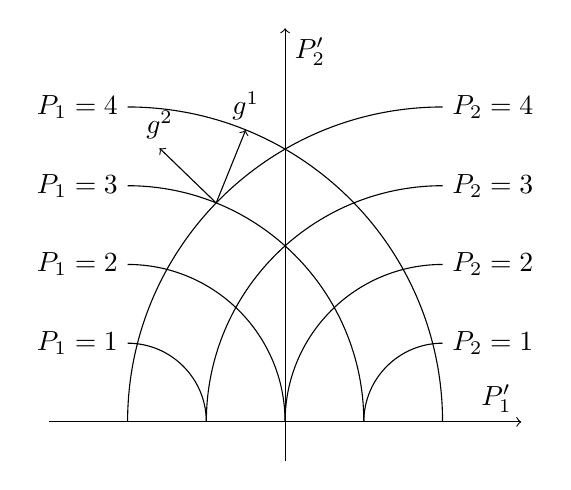
\begin{tikzpicture}
\draw[->] (-3, 0) -- (3, 0) node[anchor=south east]{\(P'_1\)};
\draw[->] (0, -0.5) -- (0, 5) node[anchor=north west]{\(P'_2\)};

\foreach \r in {1, 2, 3, 4}
	\draw[thin] (\r-2, 0) arc (0:90:\r) node[anchor=east]{\(P_1 = \r\)};

\foreach \r in {1, 2, 3, 4}
	\draw[thin] (2, \r) node[anchor=west]{\(P_2 = \r\)} arc (90:180:\r);

\draw[->] (-0.875, 2.781) -- (-0.875 + 0.375, 2.781 + 0.927) node[anchor=south]{\(\vect{g}^1\)};
\draw[->] (-0.875, 2.781) -- (-0.875 - 0.719, 2.781 + 0.695) node[anchor=south]{\(\vect{g}^2\)};
\end{tikzpicture}
 

\subsection{Kontravariantní vektory}

Mějme křivku \(P = \Gamma(t)\) v~souřadnicích \(P\), která je v~kartézských souřadnicích \(P'\) vyjádřena funkcí \(P' = \Gamma'(t) = p'(\Gamma_1(t), ..., \Gamma_n(t))\). Vyjádřeme první derivace souřadnic této křivky podle parametru \(t\):

\begin{equation}
\begin{split}
\frac{\partial \Gamma'_i}{\partial t} = \frac{\partial}{\partial t} p'_i(\Gamma_1(t), ..., \Gamma_n(t)) = \sum_{j=1}^n \frac{\partial p'_i}{P_j} (\Gamma_1(t), ..., \Gamma_n(t)) \cdot \frac{\partial \Gamma_j}{\partial t} = \\
\sum_{j=1}^n \frac{\partial \Gamma_j}{\partial t} \cdot \frac{\partial P'_i}{\partial P_j}
\end{split}
\end{equation}

Vidíme, že máme-li \(n\)-tici čísel \(\vect{u} = (u_1, u_2, ..., u_n) = \left( \frac{\partial \Gamma_1}{\partial t}, \frac{\partial \Gamma_2}{\partial t}, ..., \frac{\partial \Gamma_n}{\partial t} \right)\) v~soustavě souřadnic \(P\), tak ji do kartézské soustavy souřadnic \(P'\) transformujeme vztahem:

\begin{equation}
\label{eq:kontravariantni_vektor}
u'^i = \sum_{j=1}^n \frac{\partial p'_i}{\partial P_j} \cdot u^j = \sum_{j=1}^n \frac{\partial P'_i}{\partial P_j} \cdot u^j
\end{equation}

Každou \(n\)-tici čísel, která se transformuje podle vztahu \eqref{eq:kontravariantni_vektor} nazýváme kontravariantním vektorem. Všimněme si, že u~kontravariantních vektorů se index složky píše nahoře, aby se kontravariantní vektor odlišil od kovariantního. Nejedná se tedy o~umocňování, pokud bychom chtěli zapsat mocninu, pak mocněnec uzavřeme do závorky: \((u)^i\).

V~křivočarých souřadnicích tedy musíme rozlišovat 2 druhy vektorů, protože každý se transformuje jinak. To jsme v~kartézské soustavě souřadnic nemuseli.

Podívejme se na geometrický význam parciálních derivací \(\frac{\partial p'_i}{\partial P_j}\). Zaveďme označení \(\vect{g}_j = \left(\frac{\partial p'_1}{\partial P_j}, \frac{\partial p'_2}{\partial P_j}, ..., \frac{\partial p'_n}{\partial P_j}\right)\) pro vektor kontravariantní báze. Vektor \(\vect{g}_j\) tedy určuje, jak se změní kartézské souřadnice \(P'\), pokud změníme křivočarou souřadnici \(P_j\) o~velmi malou hodnotu. Má tedy směr tečny ke křivce \(p'(P_1, P_2, ..., t, ..., P_n)\) s~parametrem \(t\) na místě souřadnice \(P_j\).

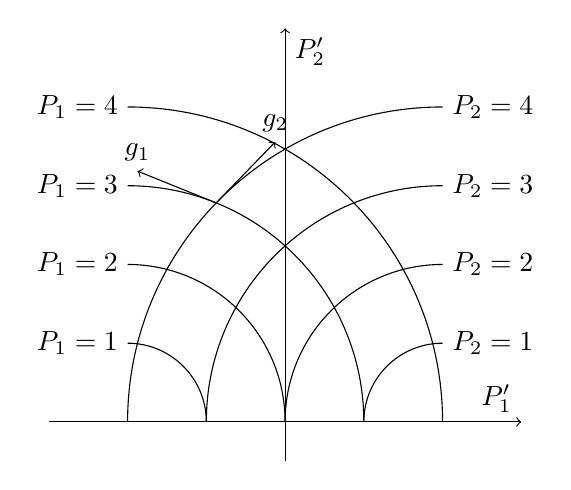
\begin{tikzpicture}
\draw[->] (-3, 0) -- (3, 0) node[anchor=south east]{\(P'_1\)};
\draw[->] (0, -0.5) -- (0, 5) node[anchor=north west]{\(P'_2\)};

\foreach \r in {1, 2, 3, 4}
	\draw[thin] (\r-2, 0) arc (0:90:\r) node[anchor=east]{\(P_1 = \r\)};

\foreach \r in {1, 2, 3, 4}
	\draw[thin] (2, \r) node[anchor=west]{\(P_2 = \r\)} arc (90:180:\r);

\draw[->] (-0.875, 2.781) -- (-0.875 - 1, 2.781 + 0.405) node[anchor=south]{\(\vect{g}_1\)};
\draw[->] (-0.875, 2.781) -- (-0.875 + 0.75, 2.781 + 0.775) node[anchor=south]{\(\vect{g}_2\)};
\end{tikzpicture}
 

\subsection{Tenzory}

Máme-li dva vektory, pak můžeme vytvořit součiny všech možných dvojic složek. Celkem tak získáme \(n^2\) součinů.

Začněme dvěma kovariantními vektory. Máme-li součin \(T_{ij} = u_i \cdot v_j\), pak transformovaný součin bude:

\begin{equation}
\label{eq:kovariantni_tenzor}
\begin{split}
T'_{ij} = u'_i \cdot v'_j = (\sum_{k=1}^n \frac{\partial p_k}{\partial P'_i} \cdot u_k) \cdot (\sum_{l=1}^n \frac{\partial p_l}{\partial P'_j} \cdot v_l) = \\
\sum_{k=1}^n \sum_{l=1}^n \frac{\partial p_k}{\partial P'_i} \cdot \frac{\partial p_l}{\partial P'_j} \cdot u_k \cdot v_l = \sum_{k=1}^n \sum_{l=1}^n \frac{\partial p_k}{\partial P'_i} \cdot \frac{\partial p_l}{\partial P'_j} \cdot T_{kl}
\end{split}
\end{equation}

Součin sum jsme prostě roznásobili. Například \((\sum_{i=1}^3 a_i) \cdot (\sum_{j=1}^3 b_j) = (a_1 + a_2 + a_3) \cdot (b_1 + b_2 + b_3) = a_1 b_1 + a_1 b_2 + a_1 b_3 + a_2 b_1 + a_2 b_2 + a_2 b_3 + a_3 b_1 + a_3 b_2 + a_3 b_3 = \sum_{i=1}^3 \sum_{j=1}^3 a_i b_i\). Každou veličinu \(T_{ij}\), která se transformuje podle vztahu \eqref{eq:kovariantni_tenzor}, nazýváme kovariantním tenzorem druhého řádu.

Máme-li součin dvou kontravariantních vektorů \(T^{ij} = u^i \cdot v^j\), pak transformovaný součin bude:

\begin{equation}
\label{eq:kontravariantni_tenzor}
\begin{split}
T'^{ij} = u'^i \cdot v'^j = (\sum_{k=1}^n \frac{\partial p'_i}{\partial P_k} \cdot u^k) \cdot (\sum_{l=1}^n \frac{\partial p'_j}{\partial P_l} \cdot v^l) = \\
\sum_{k=1}^n \sum_{l=1}^n \frac{\partial p'_i}{\partial P_k} \cdot \frac{\partial p'_j}{\partial P_l} \cdot u^k \cdot v^l = \sum_{k=1}^n \sum_{l=1}^n \frac{\partial p'_i}{\partial P_k} \cdot \frac{\partial p'_j}{\partial P_k} \cdot T^{kl}\end{split}
\end{equation}

Každou veličinu \(T^{ij}\), která se transformuje podle vztahu \eqref{eq:kontravariantni_tenzor}, nazýváme kontravariantním tenzorem druhého řádu.

Máme-li součin kovariantního a~kontravariantního \(T_i^j = u_i \cdot v^j\), pak transformovaný součin bude:

\begin{equation}
\label{eq:smyseny_tenzor}
\begin{split}
T'^j_i = u'_i \cdot v'^j = (\sum_{k=1}^n \frac{\partial p_k}{\partial P'_i} \cdot u_k) \cdot (\sum_{l=1}^n \frac{\partial p'_j}{\partial P_l} \cdot v^l) = \\
\sum_{k=1}^n \sum_{l=1}^n \frac{\partial p_k}{\partial P'_i} \cdot \frac{\partial p'_j}{\partial P_l} \cdot u_k \cdot v^l = \sum_{k=1}^n \sum_{l=1}^n \frac{\partial p_k}{\partial P'_i} \cdot \frac{\partial p'_j}{\partial P_l} \cdot T_k^l
\end{split}
\end{equation}

Každou veličinu \(T_i^j\), která se transformuje podle vztahu \eqref{eq:smyseny_tenzor}, nazýváme smýšeným tenzorem druhého řádu.

Vidíme, že se každý index tenzoru transformuje nezávisle na ostatních. To nám umožňuje definovat obecný tenzor:

\begin{fact}

Každou veličinu \(T_{ij...}^{kl...}\), která se transformuje podle vztahu~\eqref{eq:obecny_tenzor}, nazýváme tenzorem.

\begin{equation}
\label{eq:obecny_tenzor}
\begin{split}
T'^{kl...}_{ij...} = \sum_{s=1}^n \sum_{t=1}^n ... \sum_{u=1}^n \sum_{v=1}^n ... \frac{\partial p_s}{\partial P'_i} \cdot \frac{\partial p_t}{\partial P'_j} ... \cdot \frac{\partial p'_k}{\partial P_u} \cdot \frac{\partial p'_l}{\partial P_v} ... \cdot T_{st...}^{uv...} = \\
\tau_{P}^{P'} (T_{st...}^{uv...})
\end{split}
\end{equation}

\end{fact}

Počet indexů určuje řád tenzoru. Tenzor nultého řádu je skalár. Tenzor prvního řádu je kovariantní nebo kontravariantní vektor.

Zavedli jsme označení \(\tau_{P}^{P'}\) pro transformaci tenzoru ze souřadného systému \(P\) do souřadného systému \(P'\). Upozorňuji, že tato transformace není funkce, nepracuje s~jednou složkou tenzoru, ale s~celým tenzorem. Zavedli jsme ji pro zjednodušení zápisu. Povšimněme si, že tato transformace je lineárním tedy:

\begin{equation}
\label{eq:linearni_transformace_tenzoru}
\begin{split}
\alpha \cdot \tau_{P}^{P'}(S_{st...}^{uv...}) + \beta \cdot \tau_{P}^{P'}(T_{st...}^{uv...})) = \tau_{P}^{P'}(\alpha \cdot S_{st...}^{uv...} + \beta \cdot T_{st...}^{uv...})
\end{split}
\end{equation}

\subsection{Operace s~tenzory}

Prozkoumejme operace, které lze s~tenzory provádět. V~kapitole o~Euklidovském prostoru jsme operace sčítání a~násobení vektorů odvodili geometricky. V~křivočarých souřadnicích však rozdíl souřadnic dvou bodů obecně není vektor, operace s~vektory ani tenzory proto nemůžeme zavést geometricky. Můžeme je však zavést transformací do Euklidovského prostoru.

Víme, že v~Euklidovském prostoru je vztah mezi vektory a~jejich složkami lineární. Tedy že vektor \(\vect{w} = \alpha \cdot \vect{u} + \beta \cdot \vect{v}\) má složky \(w_i = \alpha \cdot u_i + \beta \cdot v_i\). Transformace \(\tau\) je lineární, takže pokud bychom soustavu souřadnic \(P\) zvolili za Euklidovskou, tak i~soustavě souřadnic \(P'\) bude platit lineární vztah mezi vektory a~jeho složkami. Pro skaláry uvedený vztah samozřejmě platí taky. Je tedy celkem přirozené, když linearitu rozšíříme na obecný tenzor:

\begin{equation}
\label{eq:scitani_a_nasobeni_tenzoru}
\begin{split}
U = \alpha \cdot S + \beta \cdot T \Leftrightarrow U_{st...}^{uv...} = \alpha \cdot S_{st...}^{uv...} + \beta \cdot T_{st...}^{uv...}
\end{split}
\end{equation}

Sčítat můžeme pouze tenzory stejného druhu, tedy tenzory se stejným počtem kovariantních a~kontravariantních indexů. Násobení tenzorů skalárem a~dříve popsané složkové násobení vektorů můžeme zobecnit na násobení dvou tenzorů. Vytvoříme součiny všech dvojic složek tenzorů:

\begin{equation}
\label{eq:nasobeni_tenzoru}
U = S \otimes T \Leftrightarrow U_{st...}^{uv...} = S_{s...}^{u...} \cdot T_{t...}^{v...}
\end{equation}

Prozkoumejme, jak se bude tento součin transformovat.

\begin{equation}
\begin{split}
U'^{kl...}_{ij...} = \tau_{P}^{P'}(S_{s...}^{u...}) \cdot \tau_{P}^{P'}(T_{t...}^{v...}) = \\
\left( \sum_{s=1}^n ... \sum_{u=1}^n ... \frac{\partial p_s}{\partial P'_i} ... \cdot \frac{\partial p'_k}{\partial P_u} ... \cdot T_{s...}^{u...} \right) \cdot \left( \sum_{t=1}^n ... \sum_{v=1}^n ... \frac{\partial p_t}{\partial P'_j} ... \cdot \frac{\partial p'_l}{\partial P_v} ... \cdot T_{t...}^{v...} \right) = \\
\sum_{s=1}^n \sum_{t=1}^n ... \sum_{u=1}^n \sum_{v=1}^n ... \frac{\partial p_s}{\partial P'_i} \cdot \frac{\partial p_t}{\partial P'_j} ... \cdot \frac{\partial p'_k}{\partial P_u} \cdot \frac{\partial p'_l}{\partial P_v} ... \cdot T_{s...}^{u...} \cdot T_{t...}^{v...} = \\
\tau_{P}^{P'}(T_{s...}^{u...} \cdot T_{t...}^{v...})
\end{split}
\end{equation}

Vidíme, že se součin tenzorů transformuje jako tenzor a~je tedy tenzorem s~počtem kovariantních indexů rovným součtu počtu kovariantních indexů součinitelů a~s~počtem kontravariantních indexů rovným součtu počtu kontravariantních indexů součinitelů. 

\subsection{Zůžení tenzoru}

V~Euklidovském prostoru jsme zavedli skalární součin vektorů. Něco obdobného bychom chtěli zavést i~v~křivočarých souřadnicích. Nejdříve však musíme vyjádřit vztah mezi derivacemi souřadnic.

Začněme tím, že vyjádříme reverzibilitu transformace souřadnic. Souřadnice \(P_i\) považujme za závislé na parametru \(t\), \(P\) tedy bude křivka.

\begin{equation}
p_k(p'_1(P_1(t), ..., P_n(t)), ..., p'_n(P_1(t), ..., P_n(t))) = P_k(t)
\end{equation}

Zderivujme rovnici podle parametru \(t\):

\begin{equation}
\label{eq:reverzibilni_derivace}
\sum_{i=1}^n \frac{\partial p_k}{\partial P'_i} \cdot \sum_{j=1}^n \frac{\partial p'_i}{\partial P_j} \cdot \frac{\partial P_j}{\partial t} = \frac{\partial P_k}{\partial t}
\end{equation}

Tato soustava rovnic musí platit pro jakoukoli sadu funkcí \(P_j\), která má definované první derivace. Zvolme tedy jednu konkrétní sadu: \(P_1 = t\), \(P_2, P_3, ..., P_n = 0\) a~vyjádřeme rovnici~\eqref{eq:reverzibilni_derivace} pro \(k = 1\):

\begin{equation}
\sum_{i=1}^n \frac{\partial p_1}{\partial P'_i} \frac{\partial p'_i}{\partial P_1} = 1
\end{equation}

Ve vnitřní sumě jsou všechny členy nulové kromě členu \(j = 1\), sumu jsme proto nahradili tímto jedním členem.
Dále vyjádřeme rovnici~\eqref{eq:reverzibilni_derivace} pro \(k = 2\):

\begin{equation}
\sum_{i=1}^n \frac{\partial p_2}{\partial P'_i} \frac{\partial p'_i}{\partial P_1} = 0
\end{equation}

Obdobně budeme postupovat pro ostatní \(k\).

Zvolme dále sadu funkcí: \(P_1 = 0\), \(P_2 = t\), \(P_3, P_4, ..., P_n = 0\) a~vyjádřeme rovnici~\eqref{eq:reverzibilni_derivace} pro \(k = 1\):

\begin{equation}
\sum_{i=1}^n \frac{\partial p_1}{\partial P'_i} \frac{\partial p'_i}{\partial P_2} = 0
\end{equation}

Pro \(k = 2\) obdržíme

\begin{equation}
\sum_{i=1}^n \frac{\partial p_2}{\partial P'_i} \frac{\partial p'_i}{\partial P_2} = 1
\end{equation}

Vidíme, že obecně pro libovolné \(k\) a~\(j\) musí platit:

\begin{equation}
\sum_{i=1}^n \frac{\partial p_k}{\partial P'_i} \frac{\partial p'_i}{\partial P_j} =
\begin{cases}
	1 \text{ pokud } k = j \\
	0 \text{ pokud } k \neq j
\end{cases}
\end{equation}

Celý výpočet si můžeme zjednodušit, pokud zavedeme Kroneckerův symbol delta:

\begin{equation}
\delta_{ij} =
\begin{cases}
	1 \text{ pokud } i = j \\
	0 \text{ pokud } i \neq j
\end{cases}
\end{equation}

Sadu funkcí \(P\) definujeme \(P_j = \delta_{jl} \cdot t\) pro zvolený parametr \(l\). Dosazením do rovnice~\eqref{eq:reverzibilni_derivace} získáme:

\begin{equation}
\label{eq:vztah_mezi_bazemi}
\begin{split}
\sum_{i=1}^n \frac{\partial p_k}{\partial P'_i} \cdot \sum_{j=1}^n \frac{\partial p'_i}{\partial P_j} \cdot \delta_{jl} = \delta_{kl} \\
\sum_{i=1}^n \frac{\partial p_k}{\partial P'_i} \cdot \frac{\partial p'_i}{\partial P_l} = \delta_{kl}
\end{split}
\end{equation}

Opět jsme nahradili vnitřní sumu jejím jediným nenulovým prvkem. Nyní můžeme přistoupit k~formulaci zúžení tenzoru. 

\begin{fact}
Mějme tenzor \(T_{ij...}^{kl...}\) s~libovolným kovariantním indexem \(i\) a~libovolným kontravariantním indexem \(k\). Pak \(S_{j...}^{l...} = \sum_{i=1}^n T_{ij...}^{il...}\) je tenzor.
\end{fact}

Při zúžení tenzoru tedy vybereme jeden kovariantní a~jeden kontravariantní index a~sečteme složky tenzoru, ve kterých jsou tyto indexy shodné. Získáme tak tenzor o~2 řády nižší.

Dokažme, že získaná veličina je opravdu tenzor tím, že prozkoumáme, jak se transformuje:

\begin{equation}
\begin{split}
T'^{kl...}_{ij...} = \tau_P^{P'} (T_{st...}^{uv...}) = \\
\sum_{s=1}^n \sum_{t=1}^n ... \sum_{u=1}^n \sum_{v=1}^n ... \frac{\partial p_s}{\partial P'_i} \cdot \frac{\partial p_t}{\partial P'_j} ... \cdot \frac{\partial p'_k}{\partial P_u} \cdot \frac{\partial p'_l}{\partial P_v} ... \cdot T_{st...}^{uv...}
\end{split}
\end{equation}

\begin{equation}
\begin{split}
S_{t...}^{v...} = \sum_{w=1}^n T_{wt...}^{wv...}
\end{split}
\end{equation}

\begin{equation}
\begin{split}
S'^{l...}_{j...} = \sum_{w=1}^n T'^{wl...}_{wj...} = \\
\sum_{w=1}^n \sum_{s=1}^n \sum_{t=1}^n ... \sum_{u=1}^n \sum_{v=1}^n ... \frac{\partial p_s}{\partial P'_w} \cdot \frac{\partial p_t}{\partial P'_j} ... \cdot \frac{\partial p'_w}{\partial P_u} \cdot \frac{\partial p'_l}{\partial P_v} ... \cdot T_{st...}^{uv...} = \\
\sum_{s=1}^n \sum_{t=1}^n ... \sum_{u=1}^n \sum_{v=1}^n ... \frac{\partial p_t}{\partial P'_j} ... \cdot \frac{\partial p'_l}{\partial P_v} ... \cdot T_{st...}^{uv...} \cdot \sum_{w=1}^n \frac{\partial p_s}{\partial P'_w} \cdot \frac{\partial p'_w}{\partial P_u} = \\
\sum_{s=1}^n \sum_{t=1}^n ... \sum_{u=1}^n \sum_{v=1}^n ... \frac{\partial p_t}{\partial P'_j} ... \cdot \frac{\partial p'_l}{\partial P_v} ... \cdot T_{st...}^{uv...} \cdot \delta_{su} = \\
\sum_{w=1}^n \sum_{t=1}^n ... \sum_{v=1}^n ... \frac{\partial p_t}{\partial P'_j} ... \cdot \frac{\partial p'_l}{\partial P_v} ... \cdot T_{wt...}^{wv...} = \\
\sum_{t=1}^n ... \sum_{v=1}^n ... \frac{\partial p_t}{\partial P'_j} ... \cdot \frac{\partial p'_l}{\partial P_v} ... \cdot S_{t...}^{v...} = \\
\tau_P^{P'} (S_{t...}^{v...})
\end{split}
\end{equation}

Pokud bychom chtěli sčítat přes dva kovariantní nebo dva kontravariantní indexy, tak by se výsledek netransformoval jako tenzor. Takovéto zůžení tedy nebudeme
vůbec uvažovat.

Zůžení nám umožňuje definovat skalární součin kovariantního a~kontravariantního vektoru jako zůžení tenzorového součinu těchto vektorů. Zavedeme při tom
konvenci, že vektor s~šipkou nad symbolem bude kontravariantní a~vektor s~šipkou pod symbolem bude kovaraintní. Pozice šipky tak bude shodná s~pozicí
indexu ve složkovém zápisu. Dále šipka nad vektorem bude odpovídat vektoru mezi dvěma body, který je také kontravariantní.

\begin{fact}
Skalární součin \(s = \kovarvect{u} \cdot \kontravect{v}\) vypočítáme podle vztahu \(s = \sum_{i=1}^n u_i \cdot v^i\).
\end{fact}

\subsection{Délka, obsah, objem}

Předpokládejme, že \(P'\) je kartézský systém souřadnic. Mějme kontravariatní vektor \(\kontravect{v'}\). Pak jeho délka bude

\begin{equation}
l = \sqrt{\sum_{i=1}^n (v'^i)^2}
\end{equation}

V~souřadném systému \(P\) bude délka vektoru \(\kontravect{v}\)

\begin{equation}
\begin{split}
l = \sqrt{\sum_{i=1}^n \left(\sum_{j=1}^n \frac{\partial p'_i}{\partial P_j} v^j \right)^2} = \sqrt{\sum_{i=1}^n \sum_{j=1}^n \sum_{k=1}^n \frac{\partial p'_i}{\partial P_j} \frac{\partial p'_i}{\partial P_k} v^j v^k} = \\
\sqrt{\sum_{j=1}^n \sum_{k=1}^n v^j v^k \sum_{i=1}^n \frac{\partial p'_i}{\partial P_j} \frac{\partial p'_i}{\partial P_k}} = \sqrt{\sum_{j=1}^n \sum_{k=1}^n g_{jk} v^j v^k}
\end{split}
\end{equation}

Zavedli jsme označení \(g_{jk} = \sum_{i=1}^n \frac{\partial p'_i}{\partial P_j} \frac{\partial p'_i}{\partial P_k} = \vect{g}_j \cdot \vect{g}_k\). Délka \(l\) je invariantní vůči změně souřadného systému. Je tedy zřejmé, že \(g_{jk}\) musí být kovariantním tenzorem druhého řádu. Jedná se o~tenzor symetrický, tedy \(g_{jk} = g_{kj}\). Nazýváme jej kovariantním metrickým tenzorem. Číselně je hodnota \(g_{jk}\) rovna skalárnímu součinu vektoru báze \(\vect{g}_j\) s~vektorem báze \(\vect{g}_k\).

Všimněme si, že vztah se velmi zjednoduší, pokud \(g_{jk} = 0\) pro \(j \neq k\):

\begin{equation}
l = \sqrt{\sum_{i=1}^n g_{ii} (v^i)^2}
\end{equation}

Vztah nám velmi připomíná rovnici~\eqref{eq:vektor_velikost}, pouze druhé mocniny složek vektoru jsou váženy vahami \(g_{ii}\). Speciálně pro diferenciály souřadnic platí:

\begin{equation}
\label{eq:delka_diferencial_souradnic}
dl = g_{ii} dx_i
\end{equation}

Tento vztah můžeme využít pro integrování podél souřadnicové osy.

Povšimněme si, že \(g_{jk}\) je pro \(j \neq k\) nulový právě tehdy, pokud jsou vektory báze \(\vect{g}_i\) vzájemně kolmé. Takovémuto souřadnému systému říkáme ortogonální. Celá řada souřadnicových systémů jsou ortogonální - například kartézský, polární, cylindrický i~sférický. Proto má smysl se jimi zabývat.

Přejděme dále k~obsahu. Mějme 2 diferenciály souřadnic \(dx_i\) a~\(dx_j\), \(i \neq j\). Potom v~ortogonálním systému souřadnic bude platit:

\begin{equation}
\label{eq:obsah_diferencial_souradnic}
dS = g_{ii} g_{jj} dx_i dx_j
\end{equation}

Vztah \eqref{eq:obsah_diferencial_souradnic} jsme odvodili jako obsah obdélníka, jehož strany jsou určeny vztahem~\eqref{eq:delka_diferencial_souradnic}. Využíváme při tom faktu, že souřadnicové osy jsou na sebe kolmé.

Obdobně můžeme vypočítat objem kvádru se stranami určenými diferenciály souřadnic \(dx_i\), \(dx_j\) a~\(dx_k\):

\begin{equation}
\label{eq:objem_diferencial_souradnic}
dV = g_{ii} g_{jj} g_{kk} dx_i dx_j dx_k
\end{equation}

Obdobně můžeme vypočítat délku kovariantního vektoru:

\begin{equation}
\begin{split}
l = \sqrt{\sum_{i=1}^n \left(\sum_{j=1}^n \frac{\partial p_j}{\partial P'_i} v_j \right)^2} = \sqrt{\sum_{i=1}^n \sum_{j=1}^n \sum_{k=1}^n \frac{\partial p_j}{\partial P'_i} \cdot \frac{\partial p_k}{\partial P'_i} v_j v_k} = \\
\sqrt{\sum_{j=1}^n \sum_{k=1}^n v_j v_k \sum_{i=1}^n} \frac{\partial p_j}{\partial P'_i} \frac{\partial p_k}{\partial P'_i} = \sqrt{\sum_{j=1}^n \sum_{k=1}^n g^{jk} v_j v_k}
\end{split}
\end{equation}

Veličinu \(g^{jk} = \sum_{i=1}^n \frac{\partial p_j}{\partial P'_i} \frac{\partial p_k}{\partial P'_i}\) nazveme kontravariantním metrickým tenzorem. Opět se jedná o~symetrický tenzor druhého řádu.


\subsection{Zpětná transformace}

Doposud jsme řešili, jak se transformují veličiny z~křivočaré soustavy souřadnic \(P\) do kartézské soustavy souřadnic \(P'\). Nyní prozkoumáme transformaci opačnou - z~kartézské soustavy souřadnic \(P\) do křivočaré soustavy souřadnic \(P'\).
Vraťme se k~rovnici \eqref{eq:vztah_mezi_bazemi}, vynásobme ji kontravariantním vektorem \(v^l\) a~proveďme sumaci přes index \(l\):
 
\begin{equation}
\label{eq:transformace_kontravariantniho_vektoru_z_kartezske_soustavy}
\begin{split}
\sum_{i=1}^n \frac{\partial p_k}{\partial P'_i} \cdot \frac{\partial p'_i}{\partial P_l} = \delta_{kl} \\
\sum_{i=1}^n \frac{\partial p_k}{\partial P'_i} \cdot \frac{\partial p'_i}{\partial P_l} v^l = \delta_{kl} \cdot v^l \\
\sum_{l=1}^n \sum_{i=1}^n \frac{\partial p_k}{\partial P'_i} \cdot \frac{\partial p'_i}{\partial P_l} v^l = \sum_{l=1}^n \delta_{kl} \cdot v^l \\
\sum_{i=1}^n \frac{\partial p_k}{\partial P'_i} \cdot \sum_{l=1}^n \frac{\partial p'_i}{\partial P_l} v^l = v^k \\
\sum_{i=1}^n \frac{\partial p_k}{\partial P'_i} v'^i = v^k
\end{split}
\end{equation}

Vidíme, že kontravariantní vektor se transformuje z~kartézské do křivočaré soustavy souřadnic jako kovariantní vektor opačným směrem. To není překvapivé uvážíme-li, že transformační funkce \(p_i\) a \(p'_i\) jsou vzájemně inverzní. Obdobně se kovariantní vektor transformuje z~kartézské do křivočaré soustavy souřadnic jako kontravariantní vektor opačným směrem:

\begin{equation}
\label{eq:transformace_kovariantniho_vektoru_z_kartezske_soustavy}
\begin{split}
\sum_{i=1}^n \frac{\partial p'_i}{\partial P_l} \cdot \frac{\partial p_k}{\partial P'_i} = \delta_{kl} \\
\sum_{i=1}^n \frac{\partial p'_i}{\partial P_l} \cdot \frac{\partial p_k}{\partial P'_i} v_k = \delta_{kl} \cdot v_k \\
\sum_{k=1}^n \sum_{i=1}^n \frac{\partial p'_i}{\partial P_l} \cdot \frac{\partial p_k}{\partial P'_i} v_k = \sum_{k=1}^n \delta_{kl} \cdot v_k \\
\sum_{i=1}^n \frac{\partial p'_i}{\partial P_l} \cdot \sum_{k=1}^n \frac{\partial p_k}{\partial P'_i} v_k = v_l \\
\sum_{i=1}^n \frac{\partial p'_i}{\partial P_l} \cdot v'_i = v_l \\
\end{split}
\end{equation}

Obdobně můžeme transformovat i~tenzory, pro každý index provedeme tuto transformaci zvlášť.

V~kartézské soustavě souřadnic ale nemusíme rozlišovat mezi kovariantními a~kontravariantními vektory, přesněji jejich složky jsou shodné. S~využitím rovnice~\eqref{eq:transformace_kovariantniho_vektoru_z_kartezske_soustavy} tak můžeme definovat transformaci kontravariantního vektoru na kovariantní tak, že kontravariantní vektor transformujeme do kartézské soustavy souřadnic a~z~té ho jako kovaraintní vektor transformujeme zpět do křivočaré soustavy souřadnic:

\begin{equation}
\begin{split}
v_l = \sum_{i=1}^n \frac{\partial p'_i}{\partial P_l} \cdot v'_i = \sum_{i=1}^n \frac{\partial p'_i}{\partial P_l} \cdot \sum_{j=1}^n \frac{\partial p'_i}{\partial P_j} v^j = \sum_{j=1}^n \sum_{i=1}^n \frac{\partial p'_i}{\partial P_l} \frac{\partial p'_i}{\partial P_j} v^j = \sum_{j=1}^n g_{lj} v^j
\end{split}
\end{equation}

Kontravariantní tenzor tedy transformujeme na kovariantní tak, že jej vynásobíme kovariantním metrickým tenzorem a~zůžíme jej (podle libovolného indexu - metrický tenzor je symetrický). Této operaci říkáme snižování indexu a~lze ji provádět pro libovolný kontravariantní index tenzoru.

Obdobně můžeme s~pomocí rovnice~\eqref{eq:transformace_kontravariantniho_vektoru_z_kartezske_soustavy} definovat transformaci kovariantního vektoru na kontravariantní:

\begin{equation}
\begin{split}
v^k = \sum_{i=1}^n \frac{\partial p_k}{\partial P'_i} v'^i = \sum_{i=1}^n \frac{\partial p_k}{\partial P'_i} \cdot \sum_{j=1}^n \frac{\partial p_j}{\partial P'_i} v_j = \sum_{j=1}^n \sum_{i=1}^n \frac{\partial p_k}{\partial P'_i} \frac{\partial p_j}{\partial P'_i} v_j = \sum_{j=1}^n g^{jk} v_j
\end{split}
\end{equation}

Vidíme, že kovariantní a~kontravariantní vektory lze mezi sebou převádět. Můžeme tedy hovořit o~vektoru \(\vect{v}\), který má kovariantní složky \(v_i\) a~kontravariantní složky \(v^i\). Této operaci říkáme zvedání indexu a~lze ji provádět pro libovolný kovariantní index tenzoru.

\subsection{Vyjádření některých operací}

Umíme-li provádět transformace vektorů, tak můžeme vyjádřit operace s~vektory v~křivočarých souřadnicích. 

\subsubsection{Skalární součin}

Začněme skalárním součinem vektorů \(\vect{u} \cdot \vect{v}\). Už víme, jak vypočítat skalární součin kovariantního a~kontravariantního vektoru. Transformací jednoho vektoru pak můžeme vypočítat skalární součin dvou vektorů stejného druhu:

\begin{fact}
\begin{equation}
\begin{split}
\kovarvect{u} \cdot \kontravect{v} = \sum_{i=1}^n u_i \cdot v^i \\
\kovarvect{u} \cdot \kovarvect{v} = \sum_{i=1}^n \sum_{j=1}^n u_i \cdot v_i \cdot g^{ij} \\
\kontravect{u} \cdot \kontravect{v} = \sum_{i=1}^n \sum_{j=1}^n u^i \cdot v^i \cdot g_{ij}
\end{split}
\end{equation}
\end{fact}

\subsubsection{Levi-Civitův symbol}

Podívejme se, jak se transformuje Levi-Civitův symbol do křivočarých souřadnic. Levi-Civitův symbol je kartézským tenzorem, můžeme jej proto transformovat na kovariantní i~kontravariantní tenzor v křivočarých souřadnicích, kde jej budeme značit \(\epsilon_{ijk}\) potažmo \(\epsilon^{ijk}\).

Začněme transformací na kovariantní tenzor. 

\begin{equation}
\begin{split}
\epsilon_{lmn} = \sum_{i=1}^3 \sum_{j=1}^3 \sum_{k=1}^3 \frac{\partial p'_i}{\partial P_l} \frac{\partial p'_j}{\partial P_m} \frac{\partial p'_k}{\partial P_n} \cdot \varepsilon_{ijk}
\end{split}
\end{equation}

Prozkoumejme, pro které indexy \(lmn\) získáme nenulové \(\epsilon_{lmn}\). Začněme situací, kdy máme 2 indexy stejné. Nechť jsou to například indexy \(l = m\). Pak

\begin{equation}
\begin{split}
\epsilon_{lln} = \sum_{i=1}^3 \sum_{j=1}^3 \sum_{k=1}^3 \frac{\partial p'_i}{\partial P_l} \frac{\partial p'_j}{\partial P_l} \frac{\partial p'_k}{\partial P_n} \cdot \varepsilon_{ijk}
\end{split}
\end{equation}

Součet členů jde přes všechny permutace indexů \(i\), \(j\) a \(k\). Proto se budou členy \(\frac{\partial p'_i}{\partial P_l} \frac{\partial p'_j}{\partial P_l} \frac{\partial p'_k}{\partial P_n}\) v~součtu vyskytovat po dvojicích s~prohozenými indexy \(i\) a \(j\). Tyto dvojice budou odpovídat sudé a~liché permutaci indexů \(i\), \(j\) a \(k\), proto symbol \(\varepsilon_{ijk}\) bude mít opačné znaménko a~všechny členy se v~součtu vyruší. Tenzor \(\epsilon_{lmn}\) proto bude mít nenulové prvky jen pro různé indexy \(l\), \(m\) a~\(n\).

Vyšetřeme tedy tenzor \(\epsilon_{lmn}\) pro různé indexy \(l\), \(m\) a~\(n\). Uvědomme si, že v~členech \(\frac{\partial p'_i}{\partial P_l} \frac{\partial p'_j}{\partial P_m} \frac{\partial p'_k}{\partial P_n}\) můžeme jednotlivé součinitele libovolně prohazovat beze změny jejich hodnot. Sou4initele proto můžeme přeskládat tak, aby členy byly ve tvaru \(\frac{\partial p'_a}{\partial P_1} \frac{\partial p'_b}{\partial P_2} \frac{\partial p'_c}{\partial P_3}\). Pokud posloupnost \([l, m, n]\) představovala sudou permutaci posloupnosti \([1, 2, 3]\), pak je potřeba sudý počet prohození součinitelů, pokud představovala permutaci lichou, pak je potřeba lichý počet prohození součinitelů. Spolu s~tím dochází ale i~k permutaci posloupností \([i, j, k]\) na posloupnosti \([a, b, c]\). Protože provádíme součet přes všechny permutace, tak budeme sčítat všechny členy i~po přeskládání součinitelů, ale při lichém počtu prohození součinitelů, tedy pokud je permutace \([l, m, n]\) lichá, je nutné násobit součinitele číslem -1. To přesně odpovídá Levi-Civitově symbolu:

\begin{equation}
\begin{split}
\epsilon_{lmn} = \left(\sum_{i=1}^3 \sum_{j=1}^3 \sum_{k=1}^3 \frac{\partial p'_i}{\partial P_1} \frac{\partial p'_j}{\partial P_2} \frac{\partial p'_k}{\partial P_3} \cdot \varepsilon_{ijk} \right) \cdot \varepsilon_{lmn} = \\
\begin{vmatrix}
  \frac{\partial p'_1}{\partial P_1} & \frac{\partial p'_2}{\partial P_1} & \frac{\partial p'_3}{\partial P_1} \\
  \frac{\partial p'_1}{\partial P_2} & \frac{\partial p'_2}{\partial P_2} & \frac{\partial p'_3}{\partial P_2} \\
  \frac{\partial p'_1}{\partial P_3} & \frac{\partial p'_2}{\partial P_3} & \frac{\partial p'_3}{\partial P_3}
\end{vmatrix}
\cdot \varepsilon_{lmn} = J \cdot \varepsilon_{lmn}
\end{split}
\end{equation}

Vidíme, že Levi-Civitův symbol se transformuje pouze násobením konstantou, tzv. Jakobiánem funkcí \(p'_i\), pro nějž jsme zavedli označení:

\begin{equation}
J = 
\begin{vmatrix}
  \frac{\partial p'_1}{\partial P_1} & \frac{\partial p'_2}{\partial P_1} & \frac{\partial p'_3}{\partial P_1} \\
  \frac{\partial p'_1}{\partial P_2} & \frac{\partial p'_2}{\partial P_2} & \frac{\partial p'_3}{\partial P_2} \\
  \frac{\partial p'_1}{\partial P_3} & \frac{\partial p'_2}{\partial P_3} & \frac{\partial p'_3}{\partial P_3}
\end{vmatrix}
\end{equation}

Obdobně můžeme transformovat Levi-Civitův symbol na kontravariantní tenzor:

\begin{equation}
\begin{split}
\epsilon^{lmn} = \sum_{i=1}^3 \sum_{j=1}^3 \sum_{k=1}^3 \frac{\partial p_l}{\partial P'_i} \frac{\partial p_m}{\partial P'_j} \frac{\partial p_n}{\partial P'_k} \cdot \varepsilon_{ijk} = \\
\left(\sum_{i=1}^3 \sum_{j=1}^3 \sum_{k=1}^3 \frac{\partial p_1}{\partial P'_i} \frac{\partial p_2}{\partial P'_j} \frac{\partial p_3}{\partial P'_k} \cdot \varepsilon_{ijk} \right) \cdot \varepsilon_{lmn} = \\
\begin{vmatrix}
  \frac{\partial p_1}{\partial P'_1} & \frac{\partial p_2}{\partial P'_1} & \frac{\partial p_3}{\partial P'_1} \\
  \frac{\partial p_1}{\partial P'_2} & \frac{\partial p_2}{\partial P'_2} & \frac{\partial p_3}{\partial P'_2} \\
  \frac{\partial p_1}{\partial P'_3} & \frac{\partial p_2}{\partial P'_3} & \frac{\partial p_3}{\partial P'_3}
\end{vmatrix}
\cdot \varepsilon_{lmn}  = J' \cdot \varepsilon_{lmn}
\end{split}
\end{equation}

Vidíme, že Levi-Civitův symbol se transformuje pouze násobením konstantou, tzv. Jakobiánem funkcí \(p_i\), pro nějž jsme zavedli označení:

\begin{equation}
J' = \begin{vmatrix}
  \frac{\partial p_1}{\partial P'_1} & \frac{\partial p_2}{\partial P'_1} & \frac{\partial p_3}{\partial P'_1} \\
  \frac{\partial p_1}{\partial P'_2} & \frac{\partial p_2}{\partial P'_2} & \frac{\partial p_3}{\partial P'_2} \\
  \frac{\partial p_1}{\partial P'_3} & \frac{\partial p_2}{\partial P'_3} & \frac{\partial p_3}{\partial P'_3}
\end{vmatrix}
\end{equation}

\subsubsection{Vektorový součin}

Prozkoumejme, jak se transformuje vektorový součin. Pro kartézské vektory platí rovnice \eqref{eq:vektorovy_soucin}, pro názornost si ji znovu připomeneme:

\begin{equation}
\begin{split}
\vect{v} = \vect{b} \times \vect{c} \\
v_i = \sum_{j=1}^3 \sum_{k=1}^3 b_j c_k \varepsilon_{ijk}
\end{split}
\end{equation}

Vidíme, že rovnice má tvar dvojího zůžení součinu vektorů \(b_j\), \(c_k\) a~tenzoru \(\varepsilon_{ijk}\). To nám umožňuje přímo zapsat vektorový součin dvou kovariantních a~dvou kontravariantních vektorů:

\begin{equation}
v^i = \sum_{j=1}^3 \sum_{k=1}^3 b_j c_k \epsilon^{ijk}
\end{equation}

\begin{equation}
v_i = \sum_{j=1}^3 \sum_{k=1}^3 b^j c^k \epsilon_{ijk}
\end{equation}

\subsubsection{Derivace vektorů}

Mějme derivaci soužky kartézského vektoru \(u_i\) podle souřadnice \(j\). Vyjádřeme ji pro kovariantní vektor:

\begin{equation}
\label{eq:derivace_vektoru}
\begin{split}
\frac{\partial u'_i}{\partial P'_j} = \frac{\partial}{\partial P'_j} \sum_{k=1}^n \frac{\partial p_k}{\partial P'_i} \cdot u_k \\
\frac{\partial}{\partial P'_j} \sum_{k=1}^n \frac{\partial p_k}{\partial P'_i}(P'_1, ..., P'_n) \cdot u_k(p_1(P'_1, ..., P'_n), ..., p_n(P'_1, ..., P'_n)) = \\
\sum_{k=1}^n \frac{\partial}{\partial P'_j} \left( \frac{\partial p_k}{\partial P'_i}(P'_1, ..., P'_n) \cdot u_k(p_1(P'_1, ..., P'_n), ..., p_n(P'_1, ..., P'_n)) \right) = \\
\sum_{k=1}^n \left(\frac{\partial p_k}{\partial P'_i} \sum_{l=1}^n \frac{\partial u_k}{\partial P_l} \cdot \frac{\partial p_l}{\partial P'_j} + \frac{\partial^2 p_k}{\partial P'_i P'_j} \cdot u_k \right) = \\
\sum_{k=1}^n \sum_{l=1}^n \frac{\partial p_k}{\partial P'_i} \frac{\partial p_l}{\partial P'_j} \frac{\partial u_k}{\partial P_l} + \sum_{k=1}^n \frac{\partial^2 p_k}{\partial P'_i P'_j} u_k
\end{split} 
\end{equation}

Vidíme, že derivace v~křivočarých souřadnicích sestává ze dvou členů. První člen odpovídá transformaci tenzoru, druhý člen odpovídá zakřivení souřadného systému. Tento druhý člen způsobuje, že derivace vektoru obecně není tenzor. Pokud ale uděláme rozdíl \(\frac{\partial u'_i}{\partial P'_j} - \frac{\partial u'_j}{\partial P'_i}\), tak se tento druhý člen vyruší a~tento rozdíl je tenzorem druhého řádu:

\begin{equation}
\label{eq:tenzor_rozdil_derivaci_vektoru}
\frac{\partial u'_i}{\partial P'_j} - \frac{\partial u'_j}{\partial P'_i} =
\sum_{k=1}^n \sum_{l=1}^n \frac{\partial p_k}{\partial P'_i} \frac{\partial p_l}{\partial P'_j} \left(\frac{\partial u_k}{\partial P_l} - \frac{\partial u_l}{\partial P_k} \right) 
\end{equation}

\section{Základní definice}

Mějme třírozměrný euklidovský prostor. Tělesem \(\Psi\) rozumíme souvislou ohraničenou množinu bodů v tomto prostoru. Hranicí tělesa rozumíme množinu bodů, které sousedí jak s~body tvořícími těleso tak i~s~body netvořícími těleso. Hranici označujeme \(\partial \Psi\). Obdobně definujeme útvar v~rovině nebo úsek na přímce. Těleso, rovinný útvar nebo úsek obecně nazveme oblast. Hranicí tělesa je uzavřená plocha, hranicí plochy je uzavřená křivka a~hranicí úseku jsou 2 body. 

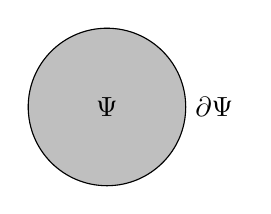
\begin{tikzpicture}
\filldraw[lightgray] (0, 0) circle (1);
\draw (0, 0) circle (1);
\draw (0, 0) node[anchor=center]{\(\Psi\)};
\draw (1, 0) node[anchor=west]{\(\partial \Psi\)};
\end{tikzpicture}

Skalární funkcí (polem) \(u(x, y)\) respektive \(u(x, y, z)\) rozumíme funkci přiřazující každému bodu \([x, y]\) v~rovině respektive \([x, y, z]\) v~prostoru skalární hodnotu. Příkladem takovéto funkce je například pole teploty nebo tlaku. Pokud není uvedeno jinak, tak uvažujeme kartézský systém souřadnic. 

Vektorovou funkcí (polem) \(\vect{u}(x, y)\) respektive \(\vect{u}(x, y, z)\) rozumíme funkci přiřazující každému bodu \([x, y]\)
 v~rovině respektive \([x, y, z]\) v~prostoru vektorovou hodnotu. Příkladem takovéto funkce je například pole rychlosti proudění kapaliny. Funkci můžeme zapsat ve složkovém tvaru \(\vect{u}=(u_x(x, y, z), u_y(x, y, z), u_z(x, y, z))\).

\section{Křivkový integrál}

Pokud máme orientovanou po částech hladkou křivku v~prostoru definovanou parametricky pomocí rovnice \eqref{eq:krivkovy_integral_krivka} a~kovariantní vektorové pole \(\kovarvect{v}\), pak křivkový integrál definujeme rovnicí \eqref{eq:krivkovy_integral_definice}.

\begin{equation}
\label{eq:krivkovy_integral_krivka}
\Gamma = (\Gamma^1(t), \Gamma^2(t), ..., \Gamma^n(t)), t \in <t_1, t_2>
\end{equation}

\begin{equation}
\label{eq:krivkovy_integral_definice}
\begin{split}
\int_\Gamma \kovarvect{v} \cdot d\kontravect{l}
\end{split}
\end{equation}

Protože \(\frac{d\kontravect{l}}{dt} = \left(\frac{d \Gamma^1}{dt}, \frac{d \Gamma^2}{dt}, ..., \frac{d \Gamma^n}{dt} \right)\), tak pro parametrickou křivku
\(\Gamma\) platí vztah \eqref{eq:krivkovy_integral_vypocet}.

\begin{equation}
\label{eq:krivkovy_integral_vypocet}
\begin{split}
\int_\Gamma \kovarvect{v} \cdot d\kontravect{l} =
\int_{t_1}^{t_2} \left(\sum_{i=1}^n v_i(\Gamma(t)) \cdot \frac{d \Gamma^i}{dt} \right) dt
\end{split}
\end{equation}

Vidíme, proč vektorové pole \(\kovarvect{v}\) musí být kovariantní. Protože diferenciály souřadnic křivky tvoří kontravariantní vektor, tak pole \(\kovarvect{v}\) musí být kovariantní, aby jejich skalární součin byl invariantní vůči změně soustavy souřadnic. Křivkový integrál je proto také invariantní vůči změně soustavy souřadnic.

Je-li křivka uzavřená (její počáteční a koncový bod jsou shodné), toto zdůrazníme kroužkem přes symbol integrálu, tedy \(\oint_\Gamma \kovarvect{v} \cdot d\kontravect{l}\), a říkáme mu cirkulace vektoru po uzavřené smyčce.

Z definice \eqref{eq:krivkovy_integral_definice} plyne, že integrujeme skalární součin hodnoty pole \(v\) a elementu dráhy \(dl\),
tedy součin průmětu pole do dráhy a elementu dráhy. Křivkový integrál proto lze použít pro výpočet práce, energie a podobně.


\subsection{Příklad}

Elektrické pole má intenzitu \(E = \left(-\frac{y}{x^2+y^2}, \frac{x}{x^2+y^2}\right) \frac{\mathrm{N}}{\mathrm{C}}\). Jakou práci pole vykoná na jednotkovém náboji, který se pohybuje po dráze \(\Gamma(t) = (1, t), t \in <-1, 1>\)?


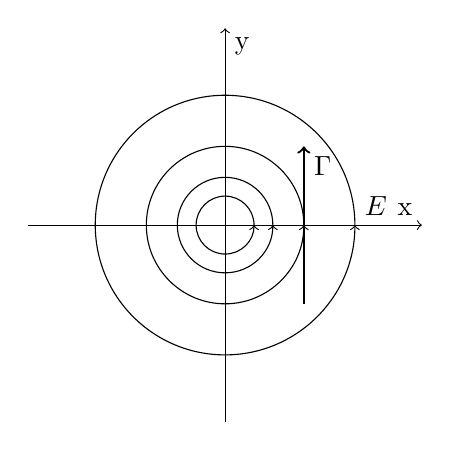
\begin{tikzpicture}
\draw[->] (-2.5, 0) -- (2.5, 0) node[anchor=south east]{x};
\draw[->] (0, -2.5) -- (0, 2.5) node[anchor=north west]{y};

\foreach \r in {0.3679, 0.6065, 1, 1.6487}
	\draw[->, thin] (\r, 0) arc (0:360:\r);
	
\draw (1.65, 0) node[anchor=south west]{\(\vect{E}\)};
	
\draw[->, thick] (1, -1) -- (1, 1) node[anchor=north west]{\(\Gamma\)};
\end{tikzpicture}


Elektrické pole působí na náboj \(Q\) silou \(\vect{F} = \vect{E} \cdot Q\). Práce vykonaná přesunutím náboje \(Q\) po dráze \(\vect{ds}\) je tedy \(dW = \vect{F} \cdot \vect{ds} = \vect{E} \cdot Q \cdot \vect{ds}\) a pro jednotkový náboj \(dW = \vect{E} \cdot \vect{ds}\). Celková práce je tedy

\[
W = \int_{-1}^1 \left (\frac{-t}{1 + t^2} \cdot 0 + \frac{1}{1 + t^2} \cdot 1 \right) = \left[\mathrm{arctg} \ t\right]_{-1}^1 = \frac{\pi}{2} \mathrm{J}
\]

\subsection{Vlastnosti křivkového integrálu}

Nyní vyšetřeme vlastnosti křivkového integrálu. Rovnice \eqref{eq:krivkovy_integral_linearita} udává linearitu křivkového integrálu. Rovnice \eqref{eq:krivkovy_integral_opacny} říká, že křivkový integrál po opačně orientované křivce je opačný. Rovnice \eqref{eq:krivkovy_integral_soucet} udává, že křivkový integrál po křivce, která je rovna součtu dvou křivek, je rovna součtu jejich křivkových integrálů. Oba dva vztahy jsou intuitivní a~lze je snadno ověřit rozepsáním integrálů pomocí vztahu \eqref{eq:krivkovy_integral_vypocet}.

\begin{equation}
\label{eq:krivkovy_integral_linearita}
\begin{split}
\int_{\Gamma} \left(\alpha \kovarvect{u} + \beta \kovarvect{v}\right) \cdot d\kontravect{l} = \alpha \int_{\Gamma} \kovarvect{u} \cdot d\kontravect{l} + \beta \int_{\Gamma} \kovarvect{v} \cdot d\kontravect{l}
\end{split}
\end{equation}

\begin{equation}
\label{eq:krivkovy_integral_opacny}
\begin{split}
\int_{-\Gamma} \kovarvect{v} \cdot d\kontravect{l} = -\int_{\Gamma} \kovarvect{v} \cdot d\kontravect{l}
\end{split}
\end{equation}

\begin{equation}
\label{eq:krivkovy_integral_soucet}
\begin{split}
\int_{\Gamma_1 + \Gamma_2} \kovarvect{v} \cdot d\kontravect{l} = \int_{\Gamma_1} \kovarvect{v} \cdot d\kontravect{l} + \int_{\Gamma_2} \kovarvect{v} \cdot d\kontravect{l}
\end{split}
\end{equation}

Protože skalární součin nezávisí na volbě soustavy souřadnic, tak ani křivkový integrál definovaný vztahem \eqref{eq:krivkovy_integral_definice} nezávisí na volbě soustavy souřadnic. Pro stejné pole a pro stejnou křivku bude křivkový integrál stejný. Je to patrné i z fyzikálního významu. Pokud bude křivkový integrál představovat celkovou práci, pak ta nezávisí na volbě soustavy souřadnic.

Máme-li uzavřenou smyčku \(\Gamma_S\), pak ji můžeme rozdělit na dvě smyčky \(\Gamma_1\) a~\(\Gamma_2\) pomocí libovolně volené přepážky \(\Gamma_P\).

\begin{tikzpicture}
\tikzmath{ \x = 0; \y = 5; }

\draw[->] (\x + 2, \y) arc (0:360:2 and 1);
\draw (\x + 2, \y) node[anchor=west]{\(\Gamma_S\)};

\tikzmath{ \x = 0; \y = 2.5; \t = 0.1; }

\draw[->] (\x + \t, \y - 1) arc (-90:90:2 and 1);
\draw[->] (\x + \t, \y + 1) -- (\x + \t, \y - 0.9);

\draw[->] (\x - \t, \y + 1) arc (90:270:2 and 1);
\draw[->] (\x - \t, \y - 0.9) -- (\x - \t, \y + 1);
\draw (\x, \y) node[anchor=west]{\(\Gamma_P\)};

\draw (\x + \t, \y - 0.9) -- (\x - \t, \y - 0.9);
\draw (\x - \t, \y - 1) -- (\x + \t, \y - 1);

\tikzmath{ \x = 0; \y = 0; \t = 0.1; }

\draw[->] (\x + \t, \y - 1) arc (-90:90:2 and 1);
\draw[->] (\x + \t, \y + 1) -- (\x + \t, \y - 1);
\draw (\x - 2, \y + 0) node[anchor=east]{\(\Gamma_1\)};

\draw[->] (\x - \t, \y + 1) arc (90:270:2 and 1);
\draw[->] (\x - \t, \y - 1) -- (\x - \t, \y + 1);
\draw (\x + 2, \y) node[anchor=west]{\(\Gamma_2\)};
\end{tikzpicture}

Přepážka je tvořena dvěma opačně orientovanými částmi křivky, které jsou nekonečně blízké. Proto se jejich příspěvky do cirkulace vyruší a platí proto vztah \eqref{eq:deleni_cirkulace}. Takto lze cirkulaci vektoru podél křivky rozdělit na součet libovolného počtu cirkulací.

\begin{equation}
\label{eq:deleni_cirkulace}
\begin{split}
\oint_{\Gamma_S} \kovarvect{v} \cdot d\kontravect{l} = \oint_{\Gamma_1} \kovarvect{v} \cdot d\kontravect{l} + \oint_{\Gamma_2} \kovarvect{v} \cdot d\kontravect{l}
\end{split}
\end{equation}

\subsection{Rotace}
\label{sec:rotace}

Vyšetřeme nyní cirkulaci vektoru nekonečně malou smyčkou. Vektorové pole \(\vect{v}\) linearizujeme podle vztahu \eqref{eq:rotace_linearizace}.
Předpokládáme, že pole pole je hladké - má derivace prvního řádu.

\begin{equation}
\label{eq:rotace_linearizace}
\vect{v} \approx \begin{pmatrix}
v_{x_0} + \frac{\partial v_x}{\partial x} \cdot x + \frac{\partial v_x}{\partial y} \cdot y + \frac{\partial v_x}{\partial z} \cdot z \\
v_{y_0} + \frac{\partial v_y}{\partial x} \cdot x + \frac{\partial v_y}{\partial y} \cdot y + \frac{\partial v_y}{\partial z} \cdot z \\
v_{z_0} + \frac{\partial v_z}{\partial x} \cdot x + \frac{\partial v_z}{\partial y} \cdot y + \frac{\partial v_z}{\partial z} \cdot z
\end{pmatrix}
\end{equation}

Dosadíme-li linearizaci \eqref{eq:rotace_linearizace} do vztahu \eqref{eq:krivkovy_integral_vypocet}, získáme vztah \eqref{eq:rotace_1}.

\begin{equation}
\label{eq:rotace_1}
\int_\Gamma \vect{v} \cdot d\vect{l} \approx
\int_{t_1}^{t_2} \begin{pmatrix}
\left(v_{x_0} + \frac{\partial v_x}{\partial x} \cdot \Gamma_x(t) + \frac{\partial v_x}{\partial y} \cdot \Gamma_y(t) + \frac{\partial v_x}{\partial z} \cdot \Gamma_z(t)\right) \cdot \frac{d \Gamma_x}{dt} + \\
\left(v_{y_0} + \frac{\partial v_y}{\partial x} \cdot \Gamma_x(t) + \frac{\partial v_y}{\partial y} \cdot \Gamma_y(t) + \frac{\partial v_y}{\partial z} \cdot \Gamma_z(t)\right) \cdot \frac{d \Gamma_y}{dt} + \\
\left(v_{z_0} + \frac{\partial v_z}{\partial x} \cdot \Gamma_x(t) + \frac{\partial v_z}{\partial y} \cdot \Gamma_y(t) + \frac{\partial v_z}{\partial z} \cdot \Gamma_z(t)\right) \cdot \frac{d \Gamma_z}{dt}
\end{pmatrix} dt
\end{equation}

Úpravou získáme vztah \eqref{eq:rotace_2}.

\begin{equation}
\label{eq:rotace_2}
\begin{matrix}
v_{x_0} \int_{t_1}^{t_2} \frac{d \Gamma_x}{dt} dt + \frac{\partial v_x}{\partial x} \int_{t_1}^{t_2} \Gamma_x(t) \frac{d \Gamma_x}{dt} dt + \frac{\partial v_x}{\partial y} \int_{t_1}^{t_2} \Gamma_y(t) \frac{d \Gamma_x}{dt} dt + \frac{\partial v_x}{\partial z} \int_{t_1}^{t_2} \Gamma_z(t) \frac{d \Gamma_x}{dt} dt + \\
v_{y_0} \int_{t_1}^{t_2} \frac{d \Gamma_y}{dt} dt + \frac{\partial v_y}{\partial x} \int_{t_1}^{t_2} \Gamma_x(t) \frac{d \Gamma_y}{dt} dt + \frac{\partial v_y}{\partial y} \int_{t_1}^{t_2} \Gamma_y(t) \frac{d \Gamma_y}{dt} dt + \frac{\partial v_y}{\partial z} \int_{t_1}^{t_2} \Gamma_z(t) \frac{d \Gamma_y}{dt} dt + \\
v_{z_0} \int_{t_1}^{t_2} \frac{d \Gamma_z}{dt} dt + \frac{\partial v_z}{\partial x} \int_{t_1}^{t_2} \Gamma_x(t) \frac{d \Gamma_z}{dt} dt + \frac{\partial v_z}{\partial y} \int_{t_1}^{t_2} \Gamma_y(t) \frac{d \Gamma_z}{dt} dt + \frac{\partial v_z}{\partial z} \int_{t_1}^{t_2} \Gamma_z(t) \frac{d \Gamma_z}{dt} dt
\end{matrix}
\end{equation}

Vyšetřeme nyní první řádek součtu. Ostatní řádky jsou obdobné.

Integrály \(\int_{t_1}^{t_2} \frac{d \Gamma_x}{dt} dt\) a \(\int_{t_1}^{t_2} \Gamma_x(t) \frac{d \Gamma_x}{dt} dt\) jsou integrály typu \(\int_{t_1}^{t_2} \mathrm{f}(\Gamma_x(t)) \frac{d \Gamma_x}{dt} dt\). Zavedeme-li substituci \(x = \Gamma_x\), tak se integrál redukuje na \(\int_{\Gamma_x(t_1)}^{\Gamma_x(t_2)} \mathrm{f}(x) dx\) a protože je smyčka \(\Gamma\) uzavřená, tak jsou obě integrační meze shodné, tedy \(\Gamma_x(t_1) = \Gamma_x(t_2)\). Proto pro uzavřenou smyčku \(\Gamma\) platí \(\int_{t_1}^{t_2} \mathrm{f}(\Gamma_x(t)) \frac{d \Gamma_x}{dt} dt = 0\).

Dále je tu integrál \(\int_{t_1}^{t_2} \Gamma_z(t) \frac{d \Gamma_x}{dt} dt\). Na obrázku \ref{img:rot_szx} je vidět význam součinu \(\Gamma_y d \Gamma_x\). Jedná se o plochu pod průmětem křivky \(\Gamma\) do roviny \(xz\). Plocha je kladná na pravé části křivky a záporná na levé části. Uvedený integrál tedy představuje kladnou plochu průmětu křivky \(\Gamma\) do roviny \(xz\). Tuto plochu označíme \(S_{xz}\).

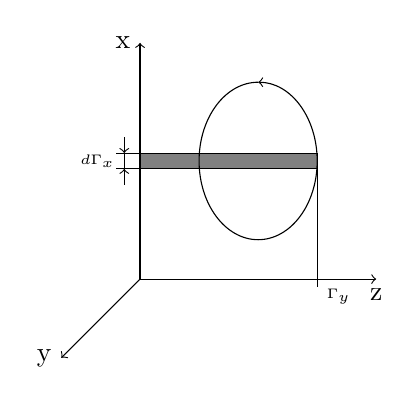
\begin{tikzpicture}
\label{img:rot_szx}
\draw[->] (0, 0) -- (3, 0);
\draw (3, 0) node[anchor=north]{z};

\draw[->] (0, 0) -- (0, 3);
\draw (0, 3) node[anchor=east]{x};

\draw[->] (0, 0) -- (-1, -1);
\draw (-1, -1) node[anchor=east]{y};

\filldraw[color=black, fill=gray] (0, 1.4) -- (2.25, 1.4) -- (2.25, 1.6) -- (0, 1.6) -- (0, 1.4);
\draw[->] (1.5, 2.5) arc (90:450:0.75 and 1);

\draw (0, 1.4) -- (-0.3, 1.4);
\draw (0, 1.6) -- (-0.3, 1.6);

\draw[->] (-0.2, 1.2) -- (-0.2, 1.4);
\draw (-0.2, 1.4) -- (-0.2, 1.6);
\draw (-0.2, 1.5) node[anchor=east]{\tiny \(d \Gamma_x\)};
\draw[->] (-0.2, 1.8) -- (-0.2, 1.6);

\draw (2.25, 1.4) -- (2.25, -0.1);
\draw (2.25, 0) node[anchor=north west]{\tiny \(\Gamma_y\)};
\end{tikzpicture}

Obdobně integrál \(\int_{t_1}^{t_2} \Gamma_y(t) \frac{d \Gamma_x}{dt} dt\) představuje plochu průmětu křivky \(\Gamma\) do roviny \(xy\), tentokrát však zápornou. Označíme ho proto \(-S_{xy}\).

\begin{equation}
\label{eq:rotace_3}
\begin{matrix}
-\frac{\partial v_x}{\partial y} S_{xy} + \frac{\partial v_x}{\partial z} S_{xz} \\
+ \frac{\partial v_y}{\partial x} S_{xy} - \frac{\partial v_y}{\partial z} S_{yz} \\
- \frac{\partial v_z}{\partial x} S_{xz} + \frac{\partial v_z}{\partial y} S_{yz}
\end{matrix}
\end{equation}

Úpravou pak získáme vztah \eqref{eq:rotace_4}.

\begin{equation}
\label{eq:rotace_4}
\left( \frac{\partial v_z}{\partial y} - \frac{\partial v_y}{\partial z} \right) S_{yz} + \left( \frac{\partial v_x}{\partial z} - \frac{\partial v_z}{\partial x} \right) S_{xz} + \left( \frac{\partial v_y}{\partial x} - \frac{\partial v_x}{\partial y} \right) S_{xy} 
\end{equation}

Dále budeme předpokládat, že smyčka leží v rovině (to jsme doposud nemuseli). Označme jednotkovou normálu této roviny \(n\). Pak \(S_{yz} = n_x S\), \(S_{xz} = n_y S\) a \(S_{xy} = n_z S\). Dosazením do vztahu \eqref{eq:rotace_4} získáme vztah \eqref{eq:rotace_5}.

\begin{equation}
\label{eq:rotace_5}
\left( \frac{\partial v_z}{\partial y} - \frac{\partial v_y}{\partial z} \right) n_x S + \left( \frac{\partial v_x}{\partial z} - \frac{\partial v_z}{\partial x} \right) n_y S + \left( \frac{\partial v_y}{\partial x} - \frac{\partial v_x}{\partial y} \right) n_z S 
\end{equation}

Vztah můžeme přepsat na skalární součin \eqref{eq:rotace_6}.

\begin{equation}
\label{eq:rotace_6}
S \cdot \vect{n} \cdot \left(\frac{\partial v_z}{\partial y} - \frac{\partial v_y}{\partial z}, \frac{\partial v_x}{\partial z} - \frac{\partial v_z}{\partial x}, \frac{\partial v_y}{\partial x} - \frac{\partial v_x}{\partial y} \right)
\end{equation}

Vektor na pravé straně skalárního součinu ve vztahu \eqref{eq:rotace_6} závisí pouze na poli \(v\), není závislý na smyčce \(\Gamma\). Nazveme ho rotací pole \(\vect{v}\) a označíme \(\rot \ \vect{v}\). Rotaci tedy lze spočítat posle vztahu \eqref{eq:rotace_vypocet}.

\begin{equation}
\label{eq:rotace_vypocet}
u = \rot \ \vect{v} = \left(\frac{\partial v_z}{\partial y} - \frac{\partial v_y}{\partial z}, \frac{\partial v_x}{\partial z} - \frac{\partial v_z}{\partial x}, \frac{\partial v_y}{\partial x} - \frac{\partial v_x}{\partial y} \right)
\end{equation}

Chceme-li rotaci zapsat ve složkovém tvaru, tak získáme 3 rovnice:

\begin{equation}
\begin{split}
u'_1 = \frac{\partial v'_3}{\partial P'_2} - \frac{\partial v'_2}{\partial P'_3} \\
u'_2 = \frac{\partial v'_1}{\partial P'_3} - \frac{\partial v'_3}{\partial P'_1} \\
u'_3 = \frac{\partial v'_2}{\partial P'_1} - \frac{\partial v'_1}{\partial P'_2}
\end{split}
\end{equation}

Pomocí Levi-Civitova tenzoru \(\varepsilon_{ijk}\) můžeme však všechny 3 rovnice zapsat pomocí jedné.

\begin{equation}
\label{eq:rotace_tenzorova}
\begin{split}
u'_i = \sum_{j=1}^3 \sum_{k=1}^3 \varepsilon_{ijk} \cdot \frac{\partial v'_k}{\partial P'_j}
\end{split}
\end{equation}

Vyjádřeme rotaci v křivočarých souřadnicích. Vztah \eqref{eq:rotace_tenzorova} vypadá, jako dvojí zůžení tenzoru, ale bohužel parciální derivace \(\frac{\partial v_k}{\partial P_j}\) nejsou tenzorem. Vztah tedy misíme upravit tak, aby veličiny v~něm obsažené tenzory byly:

\begin{equation}
\label{eq:rotace_tenzorova_2}
\begin{split}
u'_i = \frac{1}{2} \left(\sum_{j=1}^3 \sum_{k=1}^3 \varepsilon_{ijk} \cdot \frac{\partial v'_k}{\partial P'_j} + \sum_{j=1}^3 \sum_{k=1}^3 \varepsilon_{ijk} \cdot \frac{\partial v'_k}{\partial P'_j} \right) = \\
\frac{1}{2} \left(\sum_{j=1}^3 \sum_{k=1}^3 \varepsilon_{ijk} \cdot \frac{\partial v'_k}{\partial P'_j} + \sum_{k=1}^3 \sum_{j=1}^3 \varepsilon_{ikj} \cdot \frac{\partial v'_j}{\partial P'_k} \right) = \\
\frac{1}{2} \left(\sum_{j=1}^3 \sum_{k=1}^3 \varepsilon_{ijk} \cdot \frac{\partial v'_k}{\partial P'_j} + \sum_{j=1}^3 \sum_{k=1}^3 \varepsilon_{ikj} \cdot \frac{\partial v'_j}{\partial P'_k} \right) = \\
\frac{1}{2} \left(\sum_{j=1}^3 \sum_{k=1}^3 \varepsilon_{ijk} \cdot \frac{\partial v'_k}{\partial P'_j} - \sum_{j=1}^3 \sum_{k=1}^3 \varepsilon_{ijk} \cdot \frac{\partial v'_j}{\partial P'_k} \right) = \\
\frac{1}{2} \sum_{j=1}^3 \sum_{k=1}^3 \varepsilon_{ijk} \cdot \left(\frac{\partial v'_k}{\partial P'_j} - \frac{\partial v'_j}{\partial P'_k} \right)
\end{split}
\end{equation}

V~prvním kroku jsme vztah napsali polovinu dvojnásobku vztahu \eqref{eq:rotace_tenzorova}. Ve druhém kroku jsme provedli substituci \(j \leftrightarrow k\) u~druhého členu - prohodili jsme tyto proměnné. Ve třetím kroku jsme prohodily nezávislé sumy u~druhého členu. Ve čtvrtém kroku jsme prohodily indexy \(j\) a~\(k\), proto jsme museli otočit znaménko u~sumy. Nakonec jsme oba členy spojily. Podle vztahu~\eqref{eq:tenzor_rozdil_derivaci_vektoru} je rozdíl parciálních derivací, který jsme získaly, tenzorem druhého řádu. Rovnice \eqref{eq:rotace_tenzorova_2} je proto tenzorovou rovnicí a~můžeme ji tak proto transformovat:

\begin{equation}
\label{eq:rotace_tenzorova_3}
\begin{split}
u^i = \frac{1}{2} \sum_{j=1}^3 \sum_{k=1}^3 \epsilon^{ijk} \cdot \left(\frac{\partial v_k}{\partial P_j} - \frac{\partial v_j}{\partial P_k} \right) = \\
J' \cdot \frac{1}{2} \sum_{j=1}^3 \sum_{k=1}^3 \varepsilon_{ijk} \cdot \left(\frac{\partial v_k}{\partial P_j} - \frac{\partial v_j}{\partial P_k} \right) = \\
J' \cdot \sum_{j=1}^3 \sum_{k=1}^3 \varepsilon_{ijk} \cdot \frac{\partial v_k}{\partial P_j} = \\
= \sum_{j=1}^3 \sum_{k=1}^3 \epsilon^{ijk} \cdot \frac{\partial v_k}{\partial P_j}
\end{split}
\end{equation}

V~prvním kroku jsme zapsali transformovaný vztah \eqref{eq:rotace_tenzorova_2}, pak jsme rozepsali symbol \(\epsilon_{ijk} = J' \cdot \varepsilon_{ijk}\). Dále jsme využili obdobu vztahu \eqref{eq:rotace_tenzorova_2}, ale obráceně a~pro křivočaré souřadnice. Tento postup nebudu opět opakovat. Nakonec jsme opět přešli k~\(\epsilon\). Vidíme, že rotace transformuje tak, jak bychom čekali. Bez výše uvedeného odvození se však neobejdeme.


\subsection{Stokesova věta}

Mějme plochu \(S\) ohraničenou uzavřenou smyčkou \(\partial S\). Tuto plochu můžeme rozdělit na mnoho malých plošek \(\mathrm{d}S\), které můžeme považovat za rovinné útvary ohraničené uzavřenými křivkami \(\partial \mathrm{d}S\). V sekci \ref{sec:rotace} jsme odvodili vztah \eqref{eq:stokes_ds}.

\begin{equation}
\label{eq:stokes_ds}
\oint_{\partial \mathrm{d}S} \vect{v} \cdot d\vect{l} = (\rot \ \vect{v}) \cdot \vect{n} \cdot ds
\end{equation}

Máme-li 2 sousední plošky, pak se celková cirkulace po jejich vnější hranici sčítá podle vztahu \eqref{eq:deleni_cirkulace}. Jejich příspěvky \((\rot \ \vect{v}) \cdot \vect{n}\) se prostě sčítají. Proto si můžeme dovolit obě strany rovnice \eqref{eq:stokes_ds} integrovat a získáme tak rovnici \eqref{eq:stokesova_veta}. Ta se nazývá Stokesova věta a umožňuje nám přecházet mezi plošným integrálem po ploše \(S\) a křivkovým integrálem po její hranici \(\partial S\).

\begin{equation}
\label{eq:stokesova_veta}
\oint_{\partial S} \vect{v} \cdot d\vect{l} = \int_S (\rot \ \vect{v}) \cdot \vect{n} \cdot ds
\end{equation}


\section{Tok vektoru}

Pokud máme vektorové pole definované v~prostoru, tak můžeme určit jeho tok určenou plochou. Obdobně pokud máme vektorové pole definované
 v~rovině, tak můžeme určit jeho tok určenou křivkou. V~obou případech je tento tok roven integrálu průmětů vektorů pole do normál plochy nebo křivky násobené plochou nebo délkou elementu plochy nebo křivky.
 
Pokud vektorové pole představuje rychlost proudění tekutiny, pak tok vektoru představuje celkový průtok této tekutiny plochou nebo křivkou.

\subsection{Tok vektoru plochou v prostoru - plošný integrál}

Je-li \(S = \left(S_x(t, u), S_y(t, u), S_z(t, u)\right)\) po částech hladká plocha s jednotkovou normálou \(\vect{n}\) a \(\vect{v}\) je vektorové pole,
pak plošný integrál definujeme rovnicí \eqref{eq:plosny_integral_definice}. Říkáme mu tok vektoru \(v\) plochou \(S\).


\begin{equation}
\label{eq:plosny_integral_definice}
\begin{split}
\int_S \vect{v} \cdot d\vect{s} = \int_S \vect{v} \cdot \vect{n} ds
\end{split}
\end{equation}


Povšimněme si, že vektory \(\frac{\partial S}{\partial t}\) a \(\frac{\partial S}{\partial u}\) jsou (v daném bodě) tečné k ploše \(S\). Proto vektorový součin \(\frac{\partial S}{\partial t} \times \frac{\partial S}{\partial u}\) má směr normály. Ne však nutně shodnou orientaci. Navíc \(\frac{\partial S}{\partial t} \times \frac{\partial S}{\partial u} dt \ du\) má velikot splošného elementu \(ds\). Proto lze plošný integrál až na znaménko spočítat pomocí vztahu \eqref{eq:plosny_integral_vypocet}.

\begin{equation}
\label{eq:plosny_integral_vypocet}
\begin{split}
\int_S \vect{v} \cdot \vect{n} ds = \iint_S \vect{v} \cdot \left (\frac{\partial S}{\partial t} \times \frac{\partial S}{\partial u}\right) dt \ du
\end{split}
\end{equation}

Je-li plocha uzavřená, pak toto zdůrazníme kroužkem přes symbol integrálu, tedy \(\oint_S \vect{v} \cdot d\vect{s}\). Podle konvence pak normála \(n\) míří vně z plochy.

Například zákon kontinuity toku nestlačitelné kapaliny lze zapsat \(\oint_S \vect{v} \cdot d\vect{s} = 0\). Vyjadřuje fakt, že velkový výtok vektoru rychlosti kapaliny \(v\) jakoukoli uzavřenou plochou \(S\) je nulový, tedy že se kapalina nikde neztrácí, nevyvěrá ani nestlačuje. 

\subsection{Příklad}

Rychlost kapaliny je popsána vztahem \(v = \)

\subsection{Divergence}
\label{sec:divergence}

Vyšetřeme nyní tok vektoru nekonečně malou uzavřenou plochou. Vektorové pole \(\vect{v}\) linearizujeme podle vztahu \eqref{eq:divergence_linearizace}.
Předpokládáme, že pole pole je hladké - má derivace prvního řádu.

\begin{equation}
\label{eq:divergence_linearizace}
\vect{v} \approx \begin{pmatrix}
v_{x_0} + \frac{\partial v_x}{\partial x} \cdot x + \frac{\partial v_x}{\partial y} \cdot y + \frac{\partial v_x}{\partial z} \cdot z \\
v_{y_0} + \frac{\partial v_y}{\partial x} \cdot x + \frac{\partial v_y}{\partial y} \cdot y + \frac{\partial v_y}{\partial z} \cdot z \\
v_{z_0} + \frac{\partial v_z}{\partial x} \cdot x + \frac{\partial v_z}{\partial y} \cdot y + \frac{\partial v_z}{\partial z} \cdot z
\end{pmatrix}
\end{equation}

Dosadíme je do vztahu \eqref{eq:plosny_integral_definice} a získáme tak vztah \eqref{eq:divergence_1}

\begin{equation}
\label{eq:divergence_1}
\begin{split}
\int_S \vect{v} \cdot d\vect{s} = \oint_S \begin{pmatrix}
v_{x_0} + \frac{\partial v_x}{\partial x} \cdot x + \frac{\partial v_x}{\partial y} \cdot y + \frac{\partial v_x}{\partial z} \cdot z \\
v_{y_0} + \frac{\partial v_y}{\partial x} \cdot x + \frac{\partial v_y}{\partial y} \cdot y + \frac{\partial v_y}{\partial z} \cdot z \\
v_{z_0} + \frac{\partial v_z}{\partial x} \cdot x + \frac{\partial v_z}{\partial y} \cdot y + \frac{\partial v_z}{\partial z} \cdot z
\end{pmatrix} \cdot \vect{n} \mathrm{d}s
\end{split}
\end{equation}

Rozepsáním skalárního součinu a integrálu získáme výraz \eqref{eq:divergence_2}.

\begin{equation}
\label{eq:divergence_2}
\begin{matrix}
\int_S \vect{v} \cdot d\vect{s} = \\
v_{x_0} \oint_S n_x \mathrm{d}s + \frac{\partial v_x}{\partial x} \oint_S x n_x \mathrm{d}s + \frac{\partial v_x}{\partial y} \oint_S y n_x \mathrm{d}s + \frac{\partial v_x}{\partial z} \oint_S z n_x \mathrm{d}s + \\
v_{y_0} \oint_S n_y \mathrm{d}s + \frac{\partial v_y}{\partial x} \oint_S x n_y \mathrm{d}s + \frac{\partial v_y}{\partial y} \oint_S y n_y \mathrm{d}s + \frac{\partial v_y}{\partial z} \oint_S z n_y \mathrm{d}s + \\
v_{z_0} \oint_S n_z \mathrm{d}s + \frac{\partial v_z}{\partial x} \oint_S x n_z \mathrm{d}s + \frac{\partial v_z}{\partial y} \oint_S y n_z \mathrm{d}s + \frac{\partial v_z}{\partial z} \oint_S z n_z \mathrm{d}s
\end{matrix}
\end{equation}

Rozeberme první řádek součtu ve výrazu \eqref{eq:divergence_2}. Vyskytují se zde 4 integrály a ve všech se vyskytuje člen \(n_x \mathrm{d}s\). Ten představuje obsah průmětu plochy \(\mathrm{d}s\) do roviny kolmé k ose x, tedy do roviny y-z.

Jednak je zde integrál \(\oint_S x n_x \mathrm{d}s\). Uvědomíme-li si, že \(x n_x \mathrm{d}s\) je objem obecného válce se základnou tvořenou průmětem plochy \(\mathrm{d}s\) do roviny y-z a~výškou \(x\), pak \(\oint_S x n_x \mathrm{d}s = V\) je objem tělesa ohraničeného plochou \(S\).

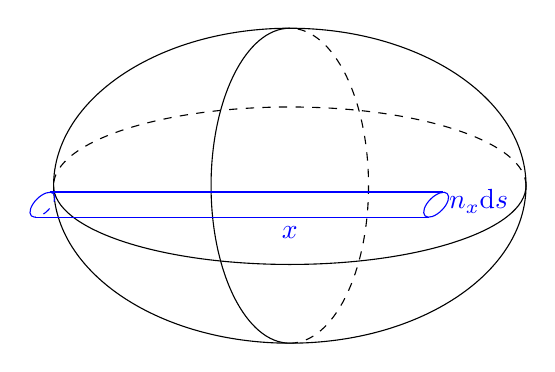
\begin{tikzpicture}
\label{img:objem}

\drawaxes{0}{0}{6}{4}{2}

\draw[thin] (5, 1) arc (0:360:3 and 2);

\draw[dashed] (5, 1) arc (0:180:3 and 1);
\draw[thin] (-1, 1) arc (180:360:3 and 1);

\draw[thin] (2, 3) arc (90:270:1 and 2);
\draw[dashed] (2, -1) arc (270:450:1 and 2);

\draw[color=blue, thin, rotate around={-45:(-1, 0.9)}] (-1, 0.9) arc (90:270:0.1 and 0.2);
\draw[color=blue, dashed, rotate around={-45:(-1, 0.9)}] (-1, 0.9) arc (90:-90:0.1 and 0.2);

\draw[color=blue, thin, rotate around={-45:(4, 0.9)}] (4, 0.9) arc (90:450:0.1 and 0.2);

\draw[color=blue, thin] (-1.05, 0.92) -- (3.95, 0.92);
\draw[color=blue, thin] (-1.23, 0.6) -- (3.77, 0.6);

\draw[color=blue] (3.9, 0.8) node[anchor=west]{\(n_x \mathrm{d}s\)};
\draw[color=blue] (2.0, 0.6) node[anchor=north]{\(x\)};

\end{tikzpicture}

Další 3 integrály jsou typu \(\oint_S f(y, z) n_x \mathrm{d}s\). Uvažujme průmět plochy \(S\) do roviny y-z. Protože je plocha \(S\) uzavřená, tak každým bodem \([y, z]\) projde sudý počet krát, přičemž v polovině případů bude normála plochy orientována v kladném směru osy x, kdy součin \(n_x \mathrm{d}s\) bude kladný, a v polovině případů bude normála plochy orientována v záporném směru osy x, kdy součin \(n_x \mathrm{d}s\) bude záporný. Protože funkce \(f(y, z)\) závisí pouze na souřadnicích \(y\) a \(z\), proto je její funkční hodnota v obou případech stejná a v integrálu se vyruší. Proto \(\oint_S f(y, z) n_x \mathrm{d}s = 0\). Zopakujeme-li uvedený postup pro všechny řádky, získáme vztah \eqref{eq:divergence_3}.

\begin{equation}
\label{eq:divergence_3}
\int_S \vect{v} \cdot d\vect{s} = \frac{\partial v_x}{\partial x} V + \frac{\partial v_y}{\partial y} V + \frac{\partial v_z}{\partial z} V = \left(\frac{\partial v_x}{\partial x} + \frac{\partial v_y}{\partial y} + \frac{\partial v_z}{\partial z}\right) V
\end{equation}
\
Ve výrazu \eqref{eq:divergence_3} se vyskytuje součet, který je závislý pouze na poli \(v\) a nazveme jej divergence pole \(v\). 

\begin{equation}
\label{eq:divergence_definice}
\diverg \vect{v} = \frac{\partial v_x}{\partial x} + \frac{\partial v_y}{\partial y} + \frac{\partial v_z}{\partial z}
\end{equation}

Divergence je definována vztahem \eqref{eq:divergence_definice} a představuje tedy výtok pole \(v\) z nekonečně malého tělesa dělená jeho objemem.

Vyjádřeme divergenci v~křivočarých souřadnicích. Začněme zápisem divergence ve složkovém tvaru:

\begin{equation}
\diverg \vect{v} = \sum_{i=1}^n \frac{\partial v_i}{\partial P'_i}
\end{equation}

Dosadíme-li za derivace vztah \eqref{eq:derivace_vektoru}, získáme:

\begin{equation}
\begin{split}
\diverg \vect{v} = \sum_{i=1}^n \sum_{k=1}^n \sum_{l=1}^n \frac{\partial p_k}{\partial P'_i} \frac{\partial p_l}{\partial P'_i} \frac{\partial v_k}{\partial P_l} + \sum_{i=1}^n \sum_{k=1}^n \frac{\partial^2 p_k}{\partial P'^2_i} v_k = \\
\sum_{k=1}^n \sum_{l=1}^n g^{kl} \frac{\partial v_k}{\partial P_l} + \sum_{i=1}^n \sum_{k=1}^n \frac{\partial^2 p_k}{\partial P'^2_i} v_k = \\
\sum_{k=1}^n \sum_{l=1}^n g^{kl} \frac{\partial v_k}{\partial P_l} + \sum_{k=1}^n v_k \cdot \sum_{i=1}^n \frac{\partial^2 p_k}{\partial P'^2_i}
\end{split}
\end{equation}

\subsection{Vlastnosti toku pole}

Vyšetřeme nyní, jak se chová tok pole při dělení plochy na menší. Mějme uzavřenou plochu \(S_S\), kterou rozdělíme libovolnou přepážkou \(S_P\) na 2 uzavřené plochy \(S_1\) a \(S_2\). Přepážka je tvořena dvěma opačně orientovanými částmi plochy, které jsou nekonečně blízké. Proto se jejich příspěvky do celkového toku vyruší a platí tak vztah \eqref{eq:deleni_toku}.

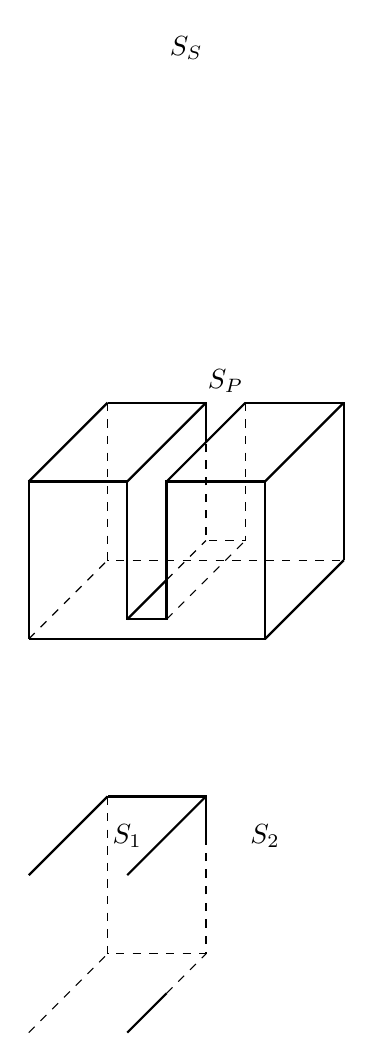
\begin{tikzpicture}
\label{img:deleni_toku}

--== One box ==--

\pgfmathsetmacro{\x}{0}
\pgfmathsetmacro{\y}{10}
\pgfmathsetmacro{\d}{1.0}

\drawaxes{\x}{\y}{4.5}{3}{2}
\drawbox{\x - 0.5}{\y - 1.5}{\x + 2.5}{\y + 0.5}{\d};

\draw (\x + 1.5, \y + 1.0) node[anchor=center]{\(S_S\)};


--== Splitted box ==--

\pgfmathsetmacro{\x}{0}
\pgfmathsetmacro{\y}{5}

\drawaxes{\x}{\y}{4.5}{3}{2}

-- Front
\draw[thick] (\x - 0.5, \y - 1.5) -- (\x + 2.5, \y - 1.5) -- (\x + 2.5, \y + 0.5) -- (\x + 1.25, \y + 0.5) -- (\x + 1.25, \y - 1.25) -- (\x + 0.75, \y - 1.25) -- (\x + 0.75, \y + 0.5) -- (\x - 0.5, \y + 0.5) -- (\x - 0.5, \y - 1.5);

\draw[dashed] (\x - 0.5 + \d, \y + 0.5 + \d) -- (\x - 0.5 + \d, \y - 1.5 + \d) -- (\x + 2.5 + \d, \y - 1.5 + \d);
\draw[thick] (\x + 2.5 + \d, \y - 1.5 + \d) -- (\x + 2.5 + \d, \y + 0.5 + \d) -- (\x + 1.25 + \d, \y + 0.5 + \d);
\draw[dashed] (\x + 1.25 + \d, \y + 0.5 + \d) -- (\x + 1.25 + \d, \y - 1.25 + \d) -- (\x + 0.75 + \d, \y - 1.25 + \d) -- (\x + 0.75 + \d, \y + 0.0 + \d);
\draw[thick] (\x + 0.75 + \d, \y + 0.0 + \d) -- (\x + 0.75 + \d, \y + 0.5 + \d) -- (\x - 0.5 + \d, \y + 0.5 + \d);

\draw[dashed] (\x - 0.5, \y - 1.5) -- (\x - 0.5 + \d, \y - 1.5 + \d);
\draw[thick] (\x + 2.5, \y - 1.5) -- (\x + 2.5 + \d, \y - 1.5 + \d);
\draw[thick] (\x + 2.5, \y + 0.5) -- (\x + 2.5 + \d, \y + 0.5 + \d);
\draw[thick] (\x + 1.25, \y + 0.5) -- (\x + 1.25 + \d, \y + 0.5 + \d);
\draw[dashed] (\x + 1.25, \y - 1.25) -- (\x + 1.25 + \d, \y - 1.25 + \d);
\draw[thick] (\x + 0.75, \y - 1.25) -- (\x + 0.75 + \d / 2, \y - 1.25 + \d / 2);
\draw[dashed] (\x + 0.75 + \d / 2, \y - 1.25 + \d / 2) -- (\x + 0.75 + \d, \y - 1.25 + \d);
\draw[thick] (\x + 0.75, \y + 0.5) -- (\x + 0.75 + \d, \y + 0.5 + \d);
\draw[thick] (\x - 0.5, \y + 0.5) -- (\x - 0.5 + \d, \y + 0.5 + \d);

\draw (\x + 2.0, \y + 1.5) node[anchor=south]{\(S_P\)};


--== Two boxes ==--

\pgfmathsetmacro{\x}{0}
\pgfmathsetmacro{\y}{0}

\drawaxes{\x}{\y}{4.5}{3}{2}

-- Front rectangle
\pgfmathsetmacro{\ax}{\x - 0.5}
\pgfmathsetmacro{\ay}{\y - 1.5}
\pgfmathsetmacro{\bx}{\x + 0.75}
\pgfmathsetmacro{\by}{\y + 0.5}
\drawrect{\ax}{\ay}{\bx}{\by}{thick};

-- Rear rectangle
\draw[dashed] (\ax + \d, \by + \d) -- (\ax + \d, \ay + \d) -- (\bx + \d, \ay + \d) -- (\bx + \d, \y + 1.0);
\draw[thick] (\bx + \d, \y + 1.0) -- (\bx + \d, \by + \d) -- (\ax + \d, \by + \d);

-- Z edges
\draw[dashed] (\ax, \ay) -- (\ax + \d, \ay + \d);
\draw[thick] (\bx, \ay) -- (\bx + \d / 2, \ay + \d / 2);
\draw[dashed] (\bx + \d / 2, \ay + \d / 2) -- (\bx + \d, \ay + \d);
\draw[thick] (\bx, \by) -- (\bx + \d, \by + \d);
\draw[thick] (\ax, \by) -- (\ax + \d, \by + \d);

\drawbox{\x + 1.25}{\y - 1.5}{\x + 2.5}{\y + 0.5}{1.0};

\draw (\x + 0.75, \y + 1.0) node[anchor=center]{\(S_1\)};
\draw (\x + 2.5, \y + 1.0) node[anchor=center]{\(S_2\)};

\end{tikzpicture}


\begin{equation}
\label{eq:deleni_toku}
\oint_{S_S} \vect{v} \cdot \mathrm{d}\vect{s} = \oint_{S_1} \vect{v} \cdot \mathrm{d}\vect{s} + \oint_{S_2} \vect{v} \cdot \mathrm{d}\vect{s}
\end{equation}


\subsection{Gaussův teorém}

Ze vztahu \eqref{eq:divergence_3} můžeme odvodit vztah \eqref{eq:gauss_dv} pro výpočet toku pole elementární uzavřenou ploškou \(\partial \mathrm{d}V\).

\begin{equation}
\label{eq:gauss_dv}
\int_{\partial \mathrm{d}V} \vect{v} \cdot d\vect{s} = \left(\diverg \ \vect{v} \right) \mathrm{d}V
\end{equation}


Podle vztahu \label{eq:deleni_toku} víme, že se toky sousedními ploškami sčítají, přičemž společné části ploch se vyruší. Proto pokud budeme integrovat
vztah \eqref{eq:gauss_dv} přes těleso \(V\), tak plošný integrál přejde na plochu po povrchu tělesa \(V\). Získáme tak Gaussův teorém \eqref{eq:gauss}.

\begin{equation}
\label{eq:gauss}
\oint_{\partial V} \vect{v} \cdot d\vect{s} = \int_V \left(\diverg \ \vect{v} \right) \mathrm{d}V
\end{equation}




\subsection{Tok vektoru křivkou v~rovině}

Je-li \(l = \left(l_x(t), l_y(t)\right)\) po částech hladká plocha s jednotkovou normálou \(\vect{n}\) a \(\vect{v}\) je vektorové pole,
pak tok vektoru \(v\) křivkou \(l\) definujeme rovnicí \eqref{eq:tok_krivkou_definice}.

\begin{equation}
\label{eq:tok_krivkou_definice}
\begin{split}
\int_l \vect{v} \cdot \vect{n} dl
\end{split}
\end{equation}

Máme-li vektor \(d \vect{l} = \left(\frac{d l_x}{dt}, \frac{d l_y}{dt}\right)\), pak vektor k~němu kolmý získáme tak, že prohodíme souřadnice a~u~jedné z~nich otočíme znaménko. Proto \(\vect{n} dl = \left(\frac{d l_y}{dt}, -\frac{d l_x}{dt}\right) dt\). Tok vektoru \(v\) křivkou \(l\) proto můžeme až na znaménko vypočítat podle vztahu \eqref{eq:tok_krivkou_vypocet}.

\begin{equation}
\label{eq:tok_krivkou_vypocet}
\begin{split}
\int_{t_1}^{t_2} \left (v_x \cdot \frac{d l_y}{dt} -v_y \cdot \frac{d l_x}{dt} \right) dt
\end{split}
\end{equation}

\subsection{Greenův teorém}

Obdobou Gaussova teorému v prostoru je Greenův teorém v rovině. Je možné jej odvodit obdobně jako Gaussův teorém.

My jej odvodíme z Gaussova teorému následující úvahou. Nechť je pole \(v\) konstantní ve směru osy \(z\). Těleso \(V\) zvolíme ve formě obecného válce, tedy libovolné podstavy protažené ve směru osy \(z\). Jeho podstavu označme \(S_P\), její hranici \(\partial S_P\) a v výšku válce \(h\).

Vyjděme z Gaussova teorému v rovnici \eqref{eq:green_1}.

\begin{equation}
\label{eq:green_1}
\oint_{\partial V} \vect{v} \cdot d\vect{s} = \int_V \left(\diverg \ \vect{v} \right) \mathrm{d}V
\end{equation}

Tok pole plochou na levé straně rovnice můžeme rozepsat na součet toku pole podstavami a pláštěm válce.
To pláštěm válce je tok hranicí podstavy násobené výškou válce, protože je pole po celé výšce konstantní. Tok podstavami je nulový, protože je pole konstantní ve směru osy \(z\) a tudíž jeho průmět do normály postavy je nulový.

Stejně tak můžeme nahradit objemový integrál na pravé straně rovnice plošným integrálem násobeným výškou. Získáme tak rovnici \eqref{eq:green_2}.

\begin{equation}
\label{eq:green_2}
h \oint_{\partial S_P} \vect{v} \cdot d\vect{l} = h \int_{S_P} \left(\diverg \ \vect{v} \right) \mathrm{d}S
\end{equation}

Podělíme-li rovnici \eqref{eq:green_2} výškou \(h\) a přejmenujeme plochu, tak získáme rovnici \eqref{eq:greenuv_teorem}. Uvědomme si, že \(\frac{\partial v_z}{\partial z} = 0\).
Proto divergence v prostoru, se kterou jsme dosud pracovali, je shodná s divergencí v rovině.

\begin{equation}
\label{eq:greenuv_teorem}
\oint_{\partial S} \vect{v} \cdot d\vect{l} = h \int_S \left(\diverg \ \vect{v} \right) \mathrm{d}S
\end{equation}

Uvedený postup je obecně použitelný, pokud máme problém definovaný v prostoru, ale v jedné nebo více os je invariantní vůči posunutí. Můžeme tak snížit
počet dimenzi problému.

\section{Změna skalárního pole v~daném směru, gradient}

Mějme skalární funkci \(\varphi(P_1, P_2, ..., P_n)\) definovanou obecně v~křivočarých souřadnicích \(P_i\). Chceme-li vypočítat její změnu v~nekonečně blízkém bodě \((P_1 + \mathrm{d}P_1, P_2 + \mathrm{d}P_2, ..., P_n + \mathrm{d}P_n)\), pak
můžeme použít vztah pro totální diferenciál funkce:

\begin{equation}
\begin{split}
\mathrm{d} \varphi = \varphi(P_1 + \mathrm{d}P_1, P_2 + \mathrm{d}P_2, ..., P_n + \mathrm{d}P_n) - \varphi(P_1, P_2, ..., P_n) = \\
\mathrm{d}P_1 \cdot \frac{\partial \varphi}{\partial P_1} + \mathrm{d}P_1 \cdot \frac{\partial \varphi}{\partial P_2} +
... + \mathrm{d}P_n \cdot \frac{\partial \varphi}{\partial P_n} = \\
\sum_{i=1}^n \mathrm{d}P_i \cdot \frac{\partial \varphi}{\partial P_i}
\end{split}
\end{equation}

Kovariantní vektor \(v_i = \frac{\partial \varphi}{\partial P_i}\) nazveme gradientem a~označíme \(\kovarvect{v} = \grad{\varphi}\). Změnu funkční hodnoty pak vypočítáme:

\begin{equation}
\begin{split}
\mathrm{d}\varphi = (\mathrm{d}P_1, \mathrm{d}P_2, ..., \mathrm{d}P_n) \cdot \grad{\varphi} 
\end{split}
\end{equation}

Dále budeme uvažovat pouze kartézský souřadný systém. V~něm víme, že skalární součin dvou vektorů nabývá svého maxima, pokud
mají oba vektory stejný směr. Gradient v~kartézském souřadném systému proto má směr nejvyššího růstu funkce \(\varphi\).

% TODO kolmá konstantní rovina


\section{Operátory}

Dále se seznámíme s operátory, které působí na pole. Již známe operátory divergence a rotace, oba působí na vektorová pole. Divergence vektorového pole
je skalární pole, které má v~každém bodě hodnotu celkového výtoku z~infinitezimálního objemu okolo daného bodu. Rotace je vektorového pole je vektorové
pole, které v každém bodě definuje cirkulaci z nekonečně malých smyček.

Další operátor je gradient. Gradient skalárního pole \(\varphi\) je vektorové pole \(\vect{v}\), které má v~každém bodě směr nejvyššího přírůstku skalárního pole, a velikost rovnou derivaci pole v tomto směru. Je definován vztahem
\[
\vect{v} = \grad \ \varphi = \left(\frac{\partial \varphi}{x}, \frac{\partial \varphi}{y}, \frac{\partial \varphi}{z}\right)
\].

Laplaceův operátor \(\Delta\) přiřazuje skalárnímu poli \(\varphi\) skalární pole \(k\) podle vztahu \(\Delta \varphi = \diverg \ \grad \ \varphi = \frac{\partial^2 \varphi}{\partial x^2} + \frac{\partial^2 \varphi}{\partial y^2} + \frac{\partial^2 \varphi}{\partial z^2}\). Operátor může působit i na vektorové pole, v tom případě působí na každou složku zvlášť. Tedy \(\Delta \ \vect{v} = \left(\Delta \ v_x, \Delta \ v_y, \Delta \ v_z \right) = \left(\frac{\partial^2 v_x}{\partial x^2} + \frac{\partial^2 v_x}{\partial y^2} + \frac{\partial^2 v_x}{\partial z^2},
\frac{\partial^2 v_y}{\partial x^2} + \frac{\partial^2 v_y}{\partial y^2} + \frac{\partial^2 v_y}{\partial z^2},
\frac{\partial^2 v_z}{\partial x^2} + \frac{\partial^2 v_z}{\partial y^2} + \frac{\partial^2 v_z}{\partial z^2} \right)\).

Vektorový Laplaceův operátor je také možné rozepsat na součet vírového a zřídlového pole jak ukazuje rovnice \eqref{eq:vect_laplace_rozepsany}.

\begin{equation}
\label{eq:vect_laplace_rozepsany}
\Delta \ \vect{v} = \grad \ \diverg \ \vect{v} - \rot \ \rot \vect{v} 
\end{equation}

\subsection{Vztahy mezi operátory}

Gradient, divergence, rotace i aplikace laplaceova operátoru jsou lineární operace. Nechť \(\alpha\) a \(\beta\) jsou konstanty, \(\varphi\) a \(rho\) skalární pole a \(u\) a \(v\) vektorová pole. Pak platí tyto vztahy:
\[
\grad(\alpha \cdot \varphi + \beta \cdot \rho) = \alpha \cdot \grad \ \varphi + \beta \cdot \grad \ \rho
\]
\[
\diverg(\alpha \cdot \vect{u} + \beta \cdot \vect{v}) = \alpha \cdot \diverg \ \vect{u} + \beta \cdot \diverg \ \vect{v}
\]
\[
\rot(\alpha \cdot \vect{u} + \beta \cdot \vect{v}) = \alpha \cdot \rot \ \vect{u} + \beta \cdot \rot \ \vect{v}
\]

Tyto vztahy lze jednoduše ověřit dosazením do jejich definic.

Dále jsou důležité následující vztahy mezi operátory.

\begin{equation}
\label{eq:div_rot}
\diverg \ \rot \ \vect{u} = 0
\end{equation}

\begin{equation}
\label{eq:rot_grad}
\rot \ \grad \ \varphi = \vect{0}
\end{equation}

\section{Pole zřídlová a vírová}

Mějme vektorové pole \(\vect{u}\) v prostoru, které má v uvažované oblasti definované derivace prvního řádu. Toto pole má obecně nenulovou divergenci a rotaci.
Pokusíme se toto pole rozložit na součet dvou polí - pole \(\vect{v}\) s nulovou rotací a pole \(\vect{w}\) s nulovou divergencí.

\begin{equation}
\vect{u} = \vect{v} + \vect{w}
\end{equation}

\begin{equation}
\rot \ \vect{v} = \vect{0}
\end{equation}

\begin{equation}
\diverg \ \vect{w} = 0
\end{equation}

To můžeme udělat tak, že stanovíme \(\vect{v} = \grad \ \varphi\). Podmínka nulové rotace je splněna, protože \(\rot \ \vect{v} = \rot \ \grad \ \varphi = \vect{0}\).
Potenciál \(\varphi\) stanovíme tak, aby \(\diverg \ \vect{u} = \diverg \ \vect{v} = \diverg \ \grad \ \varphi\). To je Poissonova rovnice bez okrajových podmínek, která má řešení popsané vztahem \eqref{eq:potencial_v_nekonecnem_prostoru}.

Pole \(\vect{w}\) je tedy \(\vect{w} = \vect{u} - \vect{v}\). Vyšetřeme jeho divergenci. \(\diverg \ \vect{w} = \diverg \ \vect{u} - \diverg \ \vect{v} = \diverg \ \vect{u} - \diverg \ \vect{u} = 0\).

Vidíme, že pole \(u\) je tedy možné rozložit na součet pole s nulovou rotací a pole s nulovou divergencí. Jak uvidíme v sekci \ref{sec:pole_virova}, tak pole
s nulovou divergencí je možné zapsat jako rotaci vektorového potenciálu. Pole \(\vect{u}\) je proto možné rozložit na součet gradientu skalárního potenciálu
a rotace vektorového potenciálu, jak popisuje rovnice \eqref{eq:rozklad_grad_rot}.

\begin{equation}
\label{eq:rozklad_grad_rot}
\vect{u} = \grad \ \varphi + \rot \vect{\psi}
\end{equation}

Podívejme se na obě složky podrobněji.

\subsection{Pole zřídlová}

Mějme pole \(v\), které má v uvažované oblasti nulovou rotaci. Pak podle Stokesovy věty cirkulace vektoru \(v\) všemi uzavřenými smyčkami v uvažované
oblasti je nulová. Mějme v oblasti 2 body A a B. Dále mějme 2 křivky \(\Gamma_1\) a \(\Gamma_2\) které obě začínají v bodě A a končí v bodě B. Pak musí platit rovnost \eqref{eq:potencial_1}. Plyne to z faktu, že otočíme-li jednu z křivek, pak jejich spojením získáme smyčku, která musí mít nulovou cirkulaci.

\begin{equation}
\label{eq:potencial_1}
\int_{\Gamma_1} \vect{v} \cdot d\vect{l} = \int_{\Gamma_2} \vect{v} \cdot d\vect{l}
\end{equation}

To ale znamená, že křivkový integrál potenciálního pole závisí pouze na počátečním a koncovém bodu, ne na tvaru křivky. Dále platí, že křivkové integrály po navazujících křivkách se sčítají. To nám umožňuje zavést skalární pole - potenciál \(\varphi\) splňující podmínku \eqref{eq:potencial_2}. Takováto pole nazýváme zřídlová, potenciální nebo také bezvírová.

\begin{equation}
\label{eq:potencial_2}
\int_{AB} \vect{v} \cdot d\vect{l} = \varphi(\vect{B}) - \varphi(\vect{A})
\end{equation}

Vyšetřeme, jaký je vztah mezi potenciálem \(\varphi\) a polem \(\vect{v}\). Nechť bod \(\vect{B}\) leží v infinitizimálně malé vzdálenosti \(dx\) od bodu
\(\vect{A}\) ve směru osy \(x\). Křivka \(AB\) bude úsečka mezi body \(\vect{A}\) a \(\vect{B}\), má tedy směr osy \(x\). Vztah \eqref{eq:potencial_2} proto lze přepsat do tvaru \eqref{eq:potencial_3}.

\begin{equation}
\label{eq:potencial_3}
\begin{split}
v_x \cdot dx = \varphi(\vect{A} + (dx, 0, 0)) - \varphi(\vect{A}) \\
v_x = \frac{\varphi(\vect{A} + (dx, 0, 0)) - \varphi(\vect{A})}{dx}
\end{split}
\end{equation}

Pro \(dx \rightarrow 0\) získáme vztah \eqref{eq:potencial_4}.

\begin{equation}
\label{eq:potencial_4}
v_x = \frac{\partial \varphi}{\partial x}
\end{equation}

Stejně budeme postupovat pro osy \(y\) a \(z\). Získáme tak vztah \eqref{eq:potencial_5}.

\begin{equation}
\label{eq:potencial_5}
\vect{v} = \left(\frac{\partial \varphi}{\partial x}, \frac{\partial \varphi}{\partial y}, \frac{\partial \varphi}{\partial z}\right) = \grad \ \varphi
\end{equation}

Vidíme tedy, že pole s nulovou rotací lze zapsat jako gradient skalárního potenciálu. Ověřme, že nulová rotace je podmínkou nutnou a postačující pro existenci
potenciálu. Snažíme se tedy dokázat, že pro dané vektorové pole \(v\) existuje potenciál \(\varphi\) takový, že \(\vect{v} = \grad \ \varphi\) tehdy a jen tehdy
pokud \(\rot \ \vect{v} = \vect{0}\).

Podmínku \(\rot \ \vect{v} = \vect{0}\) můžeme rozepsat na \(\frac{\partial v_x}{\partial y} = \frac{\partial v_y}{\partial x}\), \(\frac{\partial v_x}{\partial z} = \frac{\partial v_z}{\partial x}\) a \(\frac{\partial v_y}{\partial z} = \frac{\partial v_z}{\partial y}\).

Že se jedná o podmínku nutnou ověříme snadno. Z definice gradientu plyne \(v_x = \frac{\partial \varphi}{\partial x}\) a \(v_y = \frac{\partial \varphi}{\partial y}\). První rovnici zderivujeme podle \(y\) a získáme \(\frac{\partial v_x}{\partial y} = \frac{\partial^2 \varphi}{\partial x y}\). Druhou rovnici
zderivujeme podle \(x\) a získáme \(\frac{\partial v_y}{\partial x} = \frac{\partial^2 \varphi}{\partial y x}\). Srovnáme-li pravé strany těchto rovnic, pak
díky nezávislosti pořadí derivování jsou shodné. Proto musí platit \(\frac{\partial v_x}{\partial y} = \frac{\partial v_y}{\partial x}\). Obdobně můžeme
postupovat pro ostatní kombinace x-z a y-z a získáme tak zbylé podmínky.

Ověřit, že se jedná o podmínku postačující je poněkud složitější. Rovnice \eqref{eq:potencial_2} nám dává návod, jak potenciál určit. Zvolíme si pevný bod
v oblasti \(A\), v něm zvolíme potenciál \(\varphi_0\). Od tohoto bodu vedeme libovolnou křivku do bodu \(B\), kde hledáme potenciál. Potenciál v něm
pak spočítáme podle vztahu \eqref{eq:potencial_6}. Potenciál \(\varphi\) je tak až na konstantu \(\varphi_0\) plně určen polem \(v\).

\begin{equation}
\label{eq:potencial_6}
\varphi(\vect{B}) = \varphi_0 + \int_{AB} \vect{v} \cdot d\vect{l}
\end{equation}

Abychom ověřili, že tímto postupem skutečně dostaneme potenciál pole \(v\), tak zvolíme takovou křivku \(AB\), která nám umožní snadno spočítat gradient
potenciálu. Za bod \(A\) zvolíme počátek souřadnicového systému. Křivku \(AB\)) vedeme z počátku po ose \(x\) do vzdálenosti \(B_x\), pak ve směru osy
\(y\) do vzdálenosti \(B_y\) a nakonec ve směru osy \(z\) do vzdálenosti \(B_z\), tedy do bodu \(B\). Potenciál je tak určen vztahem \eqref{eq:potencial_7}.

\begin{equation}
\label{eq:potencial_7}
\varphi(\vect{B}) = \varphi_0 + \int_0^{B_x} v_x(x, 0, 0) dx + \int_0^{B_y} v_y(B_x, y, 0) dy  + \int_0^{B_z} v_z(B_x, B_y, z) dz
\end{equation}

Spočítejme nyní parciální derivace potenciálu \(\varphi\). Začněme derivací podle \(z\), přesněji \(B_z\). Na \(B_z\) závisí pouze poslední integrál
integrující podle \(dz\), \(B_z\) se vyskytuje v horní integrační mezi. Derivováním tohoto integrálu proto získáme vztah \eqref{eq:potencial_vz}.

\begin{equation}
\label{eq:potencial_vz}
\frac{\partial \varphi}{B_z} = v_z(B_x, B_y, B_z)
\end{equation}

Pokračujme derivací podle \(y\). \(B_y\) se vyskytuje v horní mezi druhého integrálu a dále ve třetím integrálu. Získáme tak vztah \label{eq:potencial_vy}.
Při jeho úpravě využijeme předpoklad \(\frac{\partial v_y}{\partial z} = \frac{\partial v_z}{\partial y}\).

\begin{equation}
\label{eq:potencial_vy}
\begin{split}
\frac{\partial \varphi}{B_y} = v_y(B_x, B_y, 0) + \int_0^{B_z} \frac{\partial v_z(B_x, B_y, z)}{B_y} dz = \\
v_y(B_x, B_y, 0) + \int_0^{B_z} \frac{\partial v_y(B_x, B_y, z)}{B_z} dz = \\
v_y(B_x, B_y, 0) + v_y(B_x, B_y, B_z) - v_y(B_x, B_y, 0) dz = \\
v_y(B_x, B_y, B_z)
\end{split}
\end{equation}

Nakonec spočítáme derivací podle \(x\). \(B_x\) se vyskytuje v horní mezi prvního integrálu a dále ve druhém a třetím integrálu. Získáme tak vztah \eqref{eq:potencial_vx}. Při jeho úpravě využijeme předpoklady \(\frac{\partial v_x}{\partial z} = \frac{\partial v_z}{\partial x}\) a
\(\frac{\partial v_x}{\partial y} = \frac{\partial v_y}{\partial x}\).

\begin{equation}
\label{eq:potencial_vx}
\begin{split}
\frac{\partial \varphi}{B_x} = v_x(B_x, 0, 0) + \int_0^{B_y} \frac{\partial v_y(B_x, y, 0)}{B_x} dy + \int_0^{B_z} \frac{\partial v_z(B_x, B_y, z)}{B_x} dz = \\
v_x(B_x, 0, 0) + \int_0^{B_y} \frac{\partial v_x(B_x, y, 0)}{B_y} dy + \int_0^{B_z} \frac{\partial v_x(B_x, B_y, z)}{B_z} dz = \\
v_x(B_x, 0, 0) + v_x(B_x, B_y, 0) - v_x(B_x, 0, 0) + v_x(B_x, B_y, B_z) - v_x(B_x, B_y, 0) = \\
v_x(B_x, B_y, B_z)
\end{split}
\end{equation}

Vidíme, že všechny parciální derivace potenciálu odpovídají složkám gradientu. Dokázali jsme tak, že má-li pole \(v\) nulovou rotaci, můžeme zavést jeho
potenciál vztahem \eqref{eq:potencial_7} a díky vztahu \eqref{eq:potencial_1} obecně vztahem \eqref{eq:potencial_6}.

\subsection{Pole vírová}
\label{sec:pole_virova}

Vektorová pole \(\vect{v}\) mající v celé uvažované oblasti nulovou divergenci nazýváme pole vírová. Takováto pole můžeme zapsat ve formě 
\eqref{eq:virova_pole_definice}. Veličinu \(\vect{\psi}\) nazýváme vektorovým potenciálem pole \(\vect{v}\).

\begin{equation}
\label{eq:virova_pole_definice}
\vect{v} = \rot \ \vect{\psi}
\end{equation}

Ze vztahu \eqref{eq:div_rot} je zřejmé, že nulová divergence pole \(\vect{v}\) je podmínkou nutnou pro existenci vektorového potenciálu. Že se jedná o podmínku postačující a jak potenciál určit uvidíme dále.

Z rovnice \eqref{eq:virova_pole_nejednoznacnost} je vidět, že vektorový potenciál není polem \(\vect{v}\) určen jednoznačně.
Můžeme k němu přičíst libovolné pole s nulovou rotací, tedy libovolné potenciální pole, a rovnice \eqref{eq:virova_pole_definice}
zůstane v platnosti.

\begin{equation}
\label{eq:virova_pole_nejednoznacnost}
\rot \left(\vect{\psi} + \grad \varphi \right) = \rot \ \vect{\psi} + \rot \ \grad \varphi =
\rot \ \vect{\psi} + \vect{0} = \rot \ \vect{\psi}
\end{equation}

Speciálním případem je situace, kdy \(\varphi\) zvolíme tak, že \(\diverg \vect{\psi} + \diverg \grad \varphi = 0\). To bude splněno pokud
\(-\diverg \vect{\psi} = \diverg \grad \varphi = 0\). Pravá strana rovnice představuje Poissonovu rovnici bez okrajových podmínek.
Její řešení je uvedeno dále, ale nyní je podstatná pouze jeho existence. Důsledkem tedy je, že existuje-li pole \(\vect{\psi}\) řešící
rovnici \eqref{eq:virova_pole_definice}, pak existuje \(\vect{\psi}\) takové, že má nulovou divergenci, tedy vírové pole.

Vyjdeme z rovnice \eqref{eq:virova_pole_definice}. Beze ztráty na obecnosti můžeme potenciál \(\varphi\) považovat za vírové pole.
Zaveďme tedy potenciál \(\vect{\rho}\) vztahem \(\vect{\psi} = \rot \ \vect{\rho}\). Abychom určili potenciál \(\vect{\rho}\), tak tedy
potřebujeme vyřešit rovnici \eqref{eq:virova_pole_potencial_1}.

\begin{equation}
\label{eq:virova_pole_potencial_1}
\vect{v} = \rot \ \rot \ \vect{\rho}
\end{equation}

Jak jsme viděli výše, tak můžeme zavést podmínku \(\diverg \ \vect{\rho} = 0\). Pak ale můžeme k rovnici \eqref{eq:virova_pole_potencial_1}
přičíst \(\grad \ \diverg \ \vect{\rho}\), který je nulový. Dále ještě rovnici invertujeme. Získáme tak rovnici \eqref{eq:virova_pole_potencial_2}.

\begin{equation}
\label{eq:virova_pole_potencial_2}
-\vect{v} = \grad \ \diverg \ \vect{\rho} - \rot \ \rot \ \vect{\rho}
\end{equation}

Pravou stranu rovnice můžeme přepsat podle vztahu \eqref{eq:vect_laplace_rozepsany}, získáme tak rovnici \eqref{eq:virova_pole_potencial_3}.

\begin{equation}
\label{eq:virova_pole_potencial_3}
-\vect{v} = \Delta \ \vect{\rho}
\end{equation}

To je vektorová Poissonova rovnice bez okrajových podmínek. Jak uvidíme dále, tak tato rovnice má řešení. Proto vírová pole \(v\) lze vyjádřit
pomocí pomocí rovnice \eqref{eq:virova_pole_definice} a to tak, že vyřešíme rovnici \eqref{eq:virova_pole_potencial_3} a dopočítáme \(\vect{psi} = \rot \ \vect{rho}\).

